% Chapter Template

\chapter{Magical Vectors and Where to Find Them} % Main chapter title

\label{Chapter5} % Change X to a consecutive number; for referencing this chapter elsewhere, use \ref{ChapterX}

\lhead{Chapter 5. \emph{Magical Vectors and Where to Find Them}} % Change X to a consecutive number; this is for the header on each page - perhaps a shortened title

\section{ANN Latent Space}
One of the most interesting properties of \acp{ANN} is the latent embeddings they learn, which are abstract representations of the input data. The embedding of a given data sample is the activation of the neural network at a specific layer within the network. In the case of \acp{MAE} this is the layer after which the different modalities have been merged (the embedding layer in \ref{tab:Arts_MAE_description}).

Normally when working with \acp{ANN} engineers are interested in the output of the network, for example, does the network correctly classify an image and how confident it is about the classification; this is the whole reason for using cross-entropy losses for training. However, in my case, I am more interested in how \acp{ANN} represent what they learn.

In \cite{mikolov2013distributed} and \cite{mikolov2013efficient}, it is demonstrated that skipgram models trained on large corpuses develop embeddings in the latent space of the network which tell us something about the relational meanings of the words the embeddings belong to. For example questions such as \textit{``King is to man as woman is to...?''} can be solved with some vector arithmetic on these embeddings as shown in \autoref{eqn:mikolov}.
\begin{equation}
emb(king) - emb(man) + emb(woman) \approx emb(Queen)
\label{eqn:mikolov}
\end{equation} 

The embeddings learnt by skipgram models show clusterings of different word types, such as nouns, verbs and adverbs whilst things like capital cities and country names form their own subclusters within the larger cluster of all nouns. Whilst the model does not know the meaning of any of the words it has learnt to embed, clearly it has divided the embedding space in a useful way and if symbol grounding can be performed on some of the words, this will provide a basis to start producing models which do know the meaning of the words they are embedding.

To that end, I will now demonstrate how a \ac{MAE} can be used to learn multimodal representations of words and the visual attributes they equate to in order to solve the symbol grounding problem in an unsupervised manner.

Further to this, I will show how taking an incremental approach to learning improves the quality of the bidirectional symbol grounding. Visual attibutes are more accurately described and better images are generated from descriptions by \ac{MAE} which have first been pretrained on a subset of visual attributes and descriptors compared to the randomly initialised baseline models.

\section{Vector Arithmetic}
The embeddings learnt by the \ac{MAE} can be manipulated to generate novel images using a method I developed based on the work of Mikilov et al. \cite{mikolov2013distributed, mikolov2013efficient}. For example, once the \ac{MAE} is trained, I can easily add and subtract the embeddings of images and words from one and other. \autoref{fig:vectorArthexmp} demonstrates how the embedding of an image can be changed using the embeddings of words in order to alter the colour of the image. It should be noted that this method can be applied to any attribute of the image, not just colour but also, shape, size and position, and is independant of the input modality (I can add and subtract embeddings of images or words).

\begin{figure}
\centering
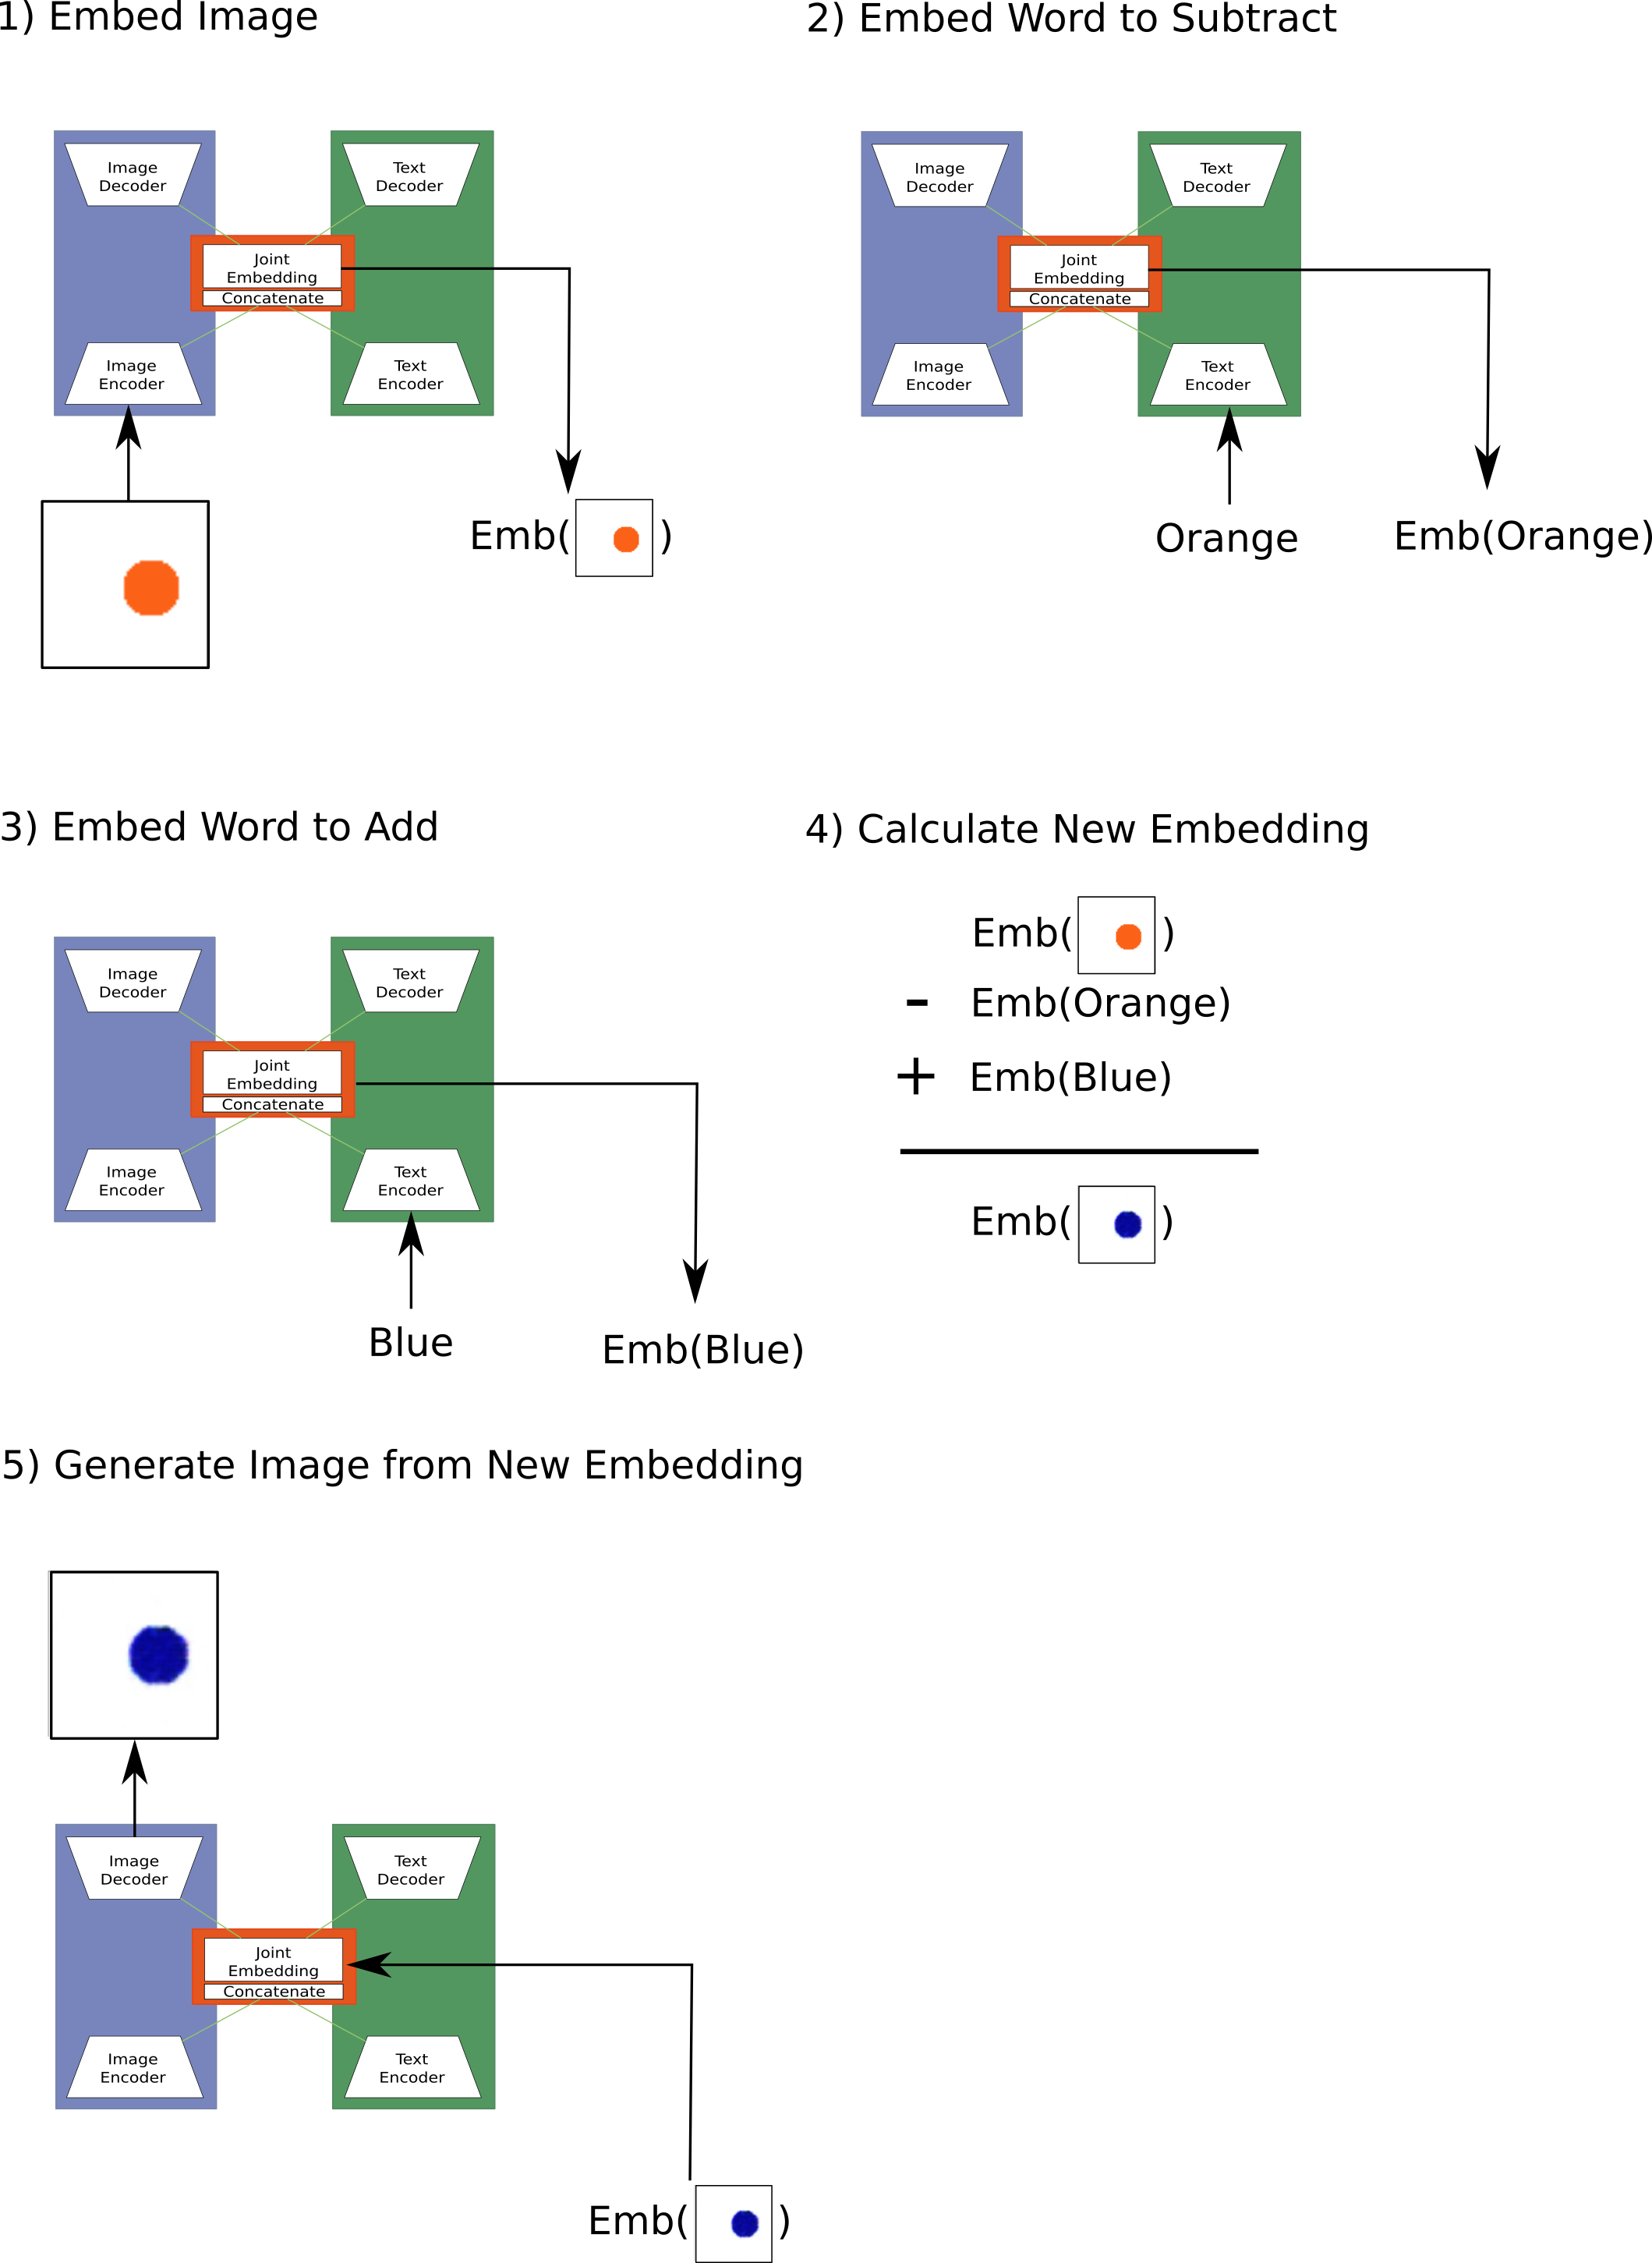
\includegraphics[width=\textwidth]{Figs/shapes/vectorArthExmp.png}
\caption{An example of how novel images can be generated using Vector Arithmetic on image and word embeddings.}
\label{fig:vectorArthexmp}
\end{figure}

\begin{figure}
\centering
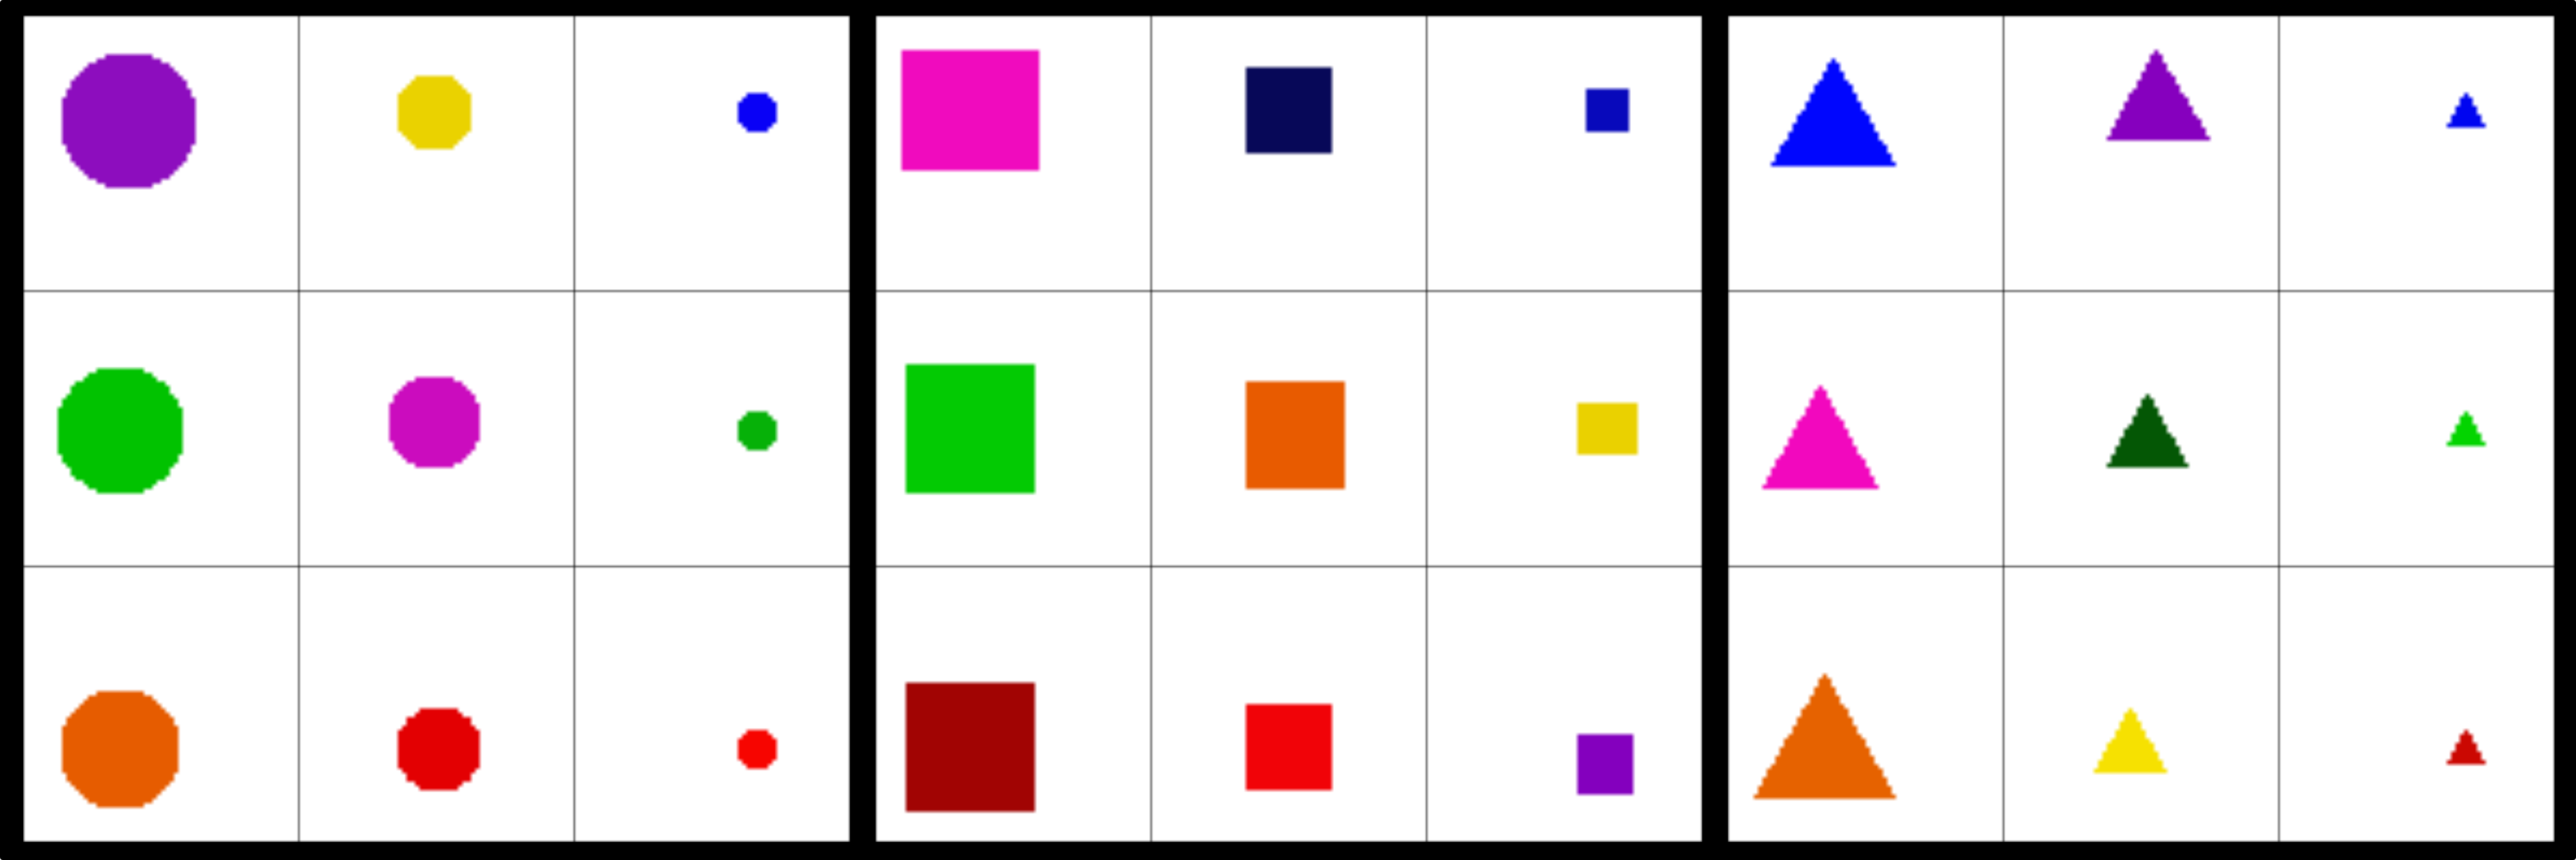
\includegraphics[width=0.75\textwidth]{Figs/shapes/shapes.png}
\caption{Examples of the different, shapes, colours, sizes and positions of objects in the ArtS dataset. The top left object would be described as ``\textsc{big indigo circle, top left}''.}
\label{fig:shapes}
\end{figure}

\newpage
\section{Artificial Shapes Dataset}
\subsection{Dataset Description}
The Artificial Shapes dataset (ArtS) contains images and simple descriptions of the images. To produce the dataset, I created a python script which generates images which are 64x64 pixels and are described by the shape, colour, size and position of the object in the image. Additionally, the \ac{RGB} value of the colour and the coordinates of the centre of the object are available, though these are not used in the following experiments. 

\begin{table}[h]
\centering
\begin{tabular}{|c|c|}
\hline
\textbf{Attribute} & \textbf{Description} \\ \hline \hline
\textbf{Shapes} & \textbf{Corners} \\ \hline
Circle (Circ) & 0\\ \hline 
Rectangle (Rect) & 4\\ \hline
Triangle (Tri)& 3\\ \hline

\textbf{Colours} & \textbf{\ac{RGB} Values}	\\ \hline	
Red (r)& (75,0,0) - (255, 10, 10)\\ \hline
Orange (o) & (225,75,0) - (255, 155, 50)\\ \hline
Yellow (y) & (230,200,0) - (255, 255, 95)\\ \hline
Green  (g)& (0,75,0) - (10, 255, 10)\\ \hline
Blue   (b)& (0,0,75) - (10, 10, 255)\\ \hline
Indigo (i)& (90,0,190) - (150, 50, 255)\\ \hline
Violet (v)& (200,0,190) - (255, 50, 255)\\ \hline 

\textbf{Sizes} & 	\textbf{Length/Radius (pixels)} \\ \hline			  
Big    (B)& 32 - 35  \\ \hline
Medium (M)& 22 - 25 \\ \hline
Small  (S)& 12 - 15 \\ \hline 

\textbf{Positions} & \textbf{Object Centre Coordinate}	\\ \hline					  
Top Left (TL)& (22,42)\\ \hline	
Top Centre (TC)& (32,42)\\ \hline
Top Right (TR)& (42,42)\\ \hline
Centre Left (CL)&(22,32)\\ \hline
Centre Centre (CC) & (32,32)\\ \hline
Centre Right (CR)&(42,32)\\ \hline
Bottom Left (BL)& (22,22)\\ \hline
Bottom Centre (BC)& (22,42)\\ \hline
Bottom Right (BR)& (42,22)\\ \hline				
\end{tabular}
\caption{Artificial Shapes dataset description.}
\label{tab:Arts_desc} 
\end{table}

To help differentiate between words, visual attributes, and the abstract concepts they represent the following notation will be used: the words of the descriptions will be written using \textsc{small capitals}, visual attributes (shapes, colours, sizes and positions) are written using \textit{Capitalised Italics}. Any other times words which could appear in the description of an image from ArtS that are not formatted as either \textsc{small capitals} or \textit{Capitalised Italics} are normal uses of these words and do not refer to either descriptions or visual attributes.
For example the word ``blue'' from a description will appear as \textsc{blue} and the colour ``blue'' will appear as \textit{Blue}. 


The dataset contains 3 different shapes, \textit{Rectangle}, \textit{Triangle} and \textit{Circle}. Each of these shapes comes in 7 colours, 3 sizes and 9 positions as described in \autoref{tab:Arts_desc}. Each colour covers a range of values, the \ac{RGB} value for each object in the ArtS dataset is randomly selected from the ranges described in the ``Description'' column of \autoref{tab:Arts_desc}. Whilst the centre of each object is fixed based on its position, the exact size is not fixed based on its size category. The size categories \textit{Big}, \textit{Medium} and \textit{Small} do not describe fixed radiuses and lengths, there is some variation in the values of these for each category.


\autoref{fig:shapes} shows some example images from the ArtS dataset for each of the 3 shapes, 7 colours, 3 sizes and 9 positions.

\subsection{Problem Description}
Using the ArtS dataset, I will demonstrate that it is possible to learn a joint, multimodal representation of the images and their descriptions. Once this representation is learnt, I will demonstrate that the \ac{MAE} can correctly label novel images with their descriptions and also that it can generate correct images from descriptions.

In the previous chapter, I showed a similar problem which was broken into two subproblems, classification and bidirectional symbol grounding. With this dataset I am not interested in performing a classification as the classification is encapsulated in the generation of correct descriptions for novel images. I will therefore be demonstrating how bidirectional symbol grounding circumvents the need for classification by providing a high level understanding of the meaning of an instance of a modality rather than just a predefined class for that instance. E.g. the \ac{ANN} is not simply assigning images of \textit{Rectangles} to the Rectangles class, but instead learns what the meanings of the word \textsc{Rectangle} and the visual property \textit{Rectangle} are. 

Further to this, I will demonstrate that once trained, the \ac{ANN} can infer the meaning of unseen descriptions to correctly generate images and vice-versa. If I omit a subcategory of object from the training data, for example blue circles, the \acp{ANN} is still able to generate images of blue circles as it has grounded the meaning of both \textsc{Blue} and \textsc{Circle} as well as the visual properties \textit{Blue} and \textit{Circle}. It is also able to correctly label images of blue circles for the same reason, despite never having never seen what a blue circle is.

\subsection{A note on Qualatitive Anaylsis of Image Generation}
As in the previous chapter, a quantitive metric for the quality of image generation is not available. However, as the data used in this chapter is more complex, I will define several terms which I use to describe the quality of image generation. These same criteria are also used in \autoref{Chapter6}.

\begin{itemize}
\item Solid - a generated image is described as being more (or less) solid depending on whether the colored pixels are more (or less) connected to one and other. E.g. if a generated image has many uncoloured pixels within the outer border of the shape, it would not be described as solid.

\item Blur - blur is used to describe whether the edges of a generated image of a shape are clearly defined or not. I.e. there is a clear boundary between the interior and exterior of a shape, with coloured pixels all occuring inside and white pixels occuring outside. This can be understood in the mathematical sense e.g. gaussian blur, where blur can be applied to an image through convolution with a guassian kernel. This operation has an averaging affect on each pixel with its neighbours leading to a smooth gradient between (in this case) coloured and white pixels and a lack of a defined edge between the shape and white background.

\item Size - the size of a generated object in an image is determined by the number of coloured pixels which are generated. Thus, big shapes should have more coloured pixels than medium shapes which in turn have more coloured pixels than small shapes.

\item Shape - if a generated shape has the (approximately) correct number of edges and corners, it is considered to be correctly generated. I.e. 4 edges and 4 corners at 90 degrees to one and other is a rectangle, 3 edges and corners at 60 degrees to one and other is a triangle and 1 edge 0 corners is a circle. Due to interactions between other image quality properties such as solidity and blur, holes might occur in the generated shapes. As such, these criteria are not strictly inforced and the evaluation is made subjectively. However, as the images are available for you (the reader) to look at, you can form your own opinion as to whether these properties have been fairly assigned.

\item Position - position is considered to be correctly learnt if the centre of the generated object appears at approximately the coordinates of that position as defined in \autoref{tab:Arts_desc}.
\end{itemize}  


\subsection{Network Description}
The overall structure of the \ac{ANN} used for the experiements in this chapter is very similar to the one used in \autoref{Chapter4}, with two inputs for each of the different modalities, this time, images and words. However, it only has two outputs, one for images and one for words, unlike in the previous chapter where I also had a third output which acted as a classification layer. \autoref{tab:Arts_MAE_description}  gives the specific details on each of the layers of the network. Additionally, batch normalisation is used between each convolution layer.

The design of the \ac{MAE} used in this chapter is deeper and wider (has more layers and more neurons in each layer) than the network used in the previous chapter. The reason for this is that the data used in this chapter is more complex, and the small network from \autoref{Chapter4} was not sufficient to achieve the quality of results demonstrated by the larger network I used in its place.

The description encoding branch of the \ac{MAE} described in \autoref{tab:Arts_MAE_description} is designed mainly to reshape the representation of the descriptions to match the shape of the image representation. The description representation is already highly abstract at the input (it is the sum of one-hot encodings of the words of the description). As such, very little effort from the \ac{MAE} is needed to extract a meaningful representation of the description, compared to the work needed to extract the same amount of meaning from the representation of the images.

\begin{table}
		\centering
		\begin{tabular}{|c|c|c|c|c|c|c|}
			\hline
			\textbf{Block} & \textbf{Layer} & \textbf{Type} & \textbf{Neurons} & \textbf{Kernel} & \textbf{Strides} & \textbf{Activation} \\ \hline
			\multirow{3}{*}{Image} & 1i	&	2D Conv & 64 & (3,3) & (1,1) & Relu \\ \cline{2-7}
			& 2i	&	2D Conv & 64 & (3,3) & (2,2) & Relu \\ \cline{2-7}
			& 3i	&	2D Conv & 32 & (3,3) & (2,2) & Relu \\ \cline{2-7}
\multirow{3}{*}{Encoder} & 4i	&	2D Conv & 16 & (3,3) & (2,2) & Relu \\ \cline{2-7}
			& 5i	&	2D Conv & 16 & (3,3) & (2,2) & Relu \\ \cline{2-7}
			& 6i	&	2D Conv & 16 & (3,3) & (2,2) & Relu \\ \cline{2-7}
			& 7i	&	Dropout p=0.25 &	 & 	     &       &  \\ \hline

			\multirow{3}{*}{Description} & 1w	& Dense & 128 & & &TanH \\ \cline{2-7}
			& 2w	& Dense & 256 & & &TanH \\ \cline{2-7}
			& 3w 	&	Dropout p=0.5 &	 & 	     &       & \\ \cline{2-7}
\multirow{4}{*}{Encoder}& 4w  &	Reshape (16,16,1) & & & & \\ \cline{2-7}
			& 5w	&	2D Conv & 16 & (3,3) & (2,2) & Relu \\ \cline{2-7}
			& 6w	&	2D Conv & 16 & (3,3) & (2,2) & Relu \\ \cline{2-7}
			& 7w	&	2D Conv & 16 & (3,3) & (2,2) & Relu \\ \hline

			Merge & 8iw	& Merge & & & & \\ \hline
Embedding & 9iw	&	2D Conv  & emb size & (3,3) & (1,1) & Relu \\ \hline
			
			
			\multirow{4}{*}{Image} & 10i 	&	Dropout p=0.25 &	 & 	     &       & \\ \cline{2-7}
			& 11i	&	2D Trans Conv & 16 & (3,3) & (2,2)  & TanH \\ \cline{2-7}
			& 12i	&	2D Trans Conv & 16 & (3,3) & (2,2)  & TanH \\ \cline{2-7}
			& 13i	&	2D Trans Conv & 16 & (3,3) & (2,2)  & TanH \\ \cline{2-7}
\multirow{4}{*}{Decoder}& 14i	&	2D Trans Conv & 32 & (3,3) & (1,1)  & TanH \\ \cline{2-7}
			& 15i	&	2D Trans Conv & 64 & (3,3) & (1,1)  & TanH \\ \cline{2-7}
			& 16i	&	2D Trans Conv & 64 & (3,3) & (1,1)  & TanH \\ \cline{2-7}
			& 17i	&	2D Trans Conv & 3 & (3,3) & (1,1) & Sigmoid\\ \hline 

			\multirow{4}{*}{Description} & 10w 	&	Dropout p=0.25 &	 & 	     &       & \\ \cline{2-7}
			& 12w	&	2D Trans Conv & 16 & (3,3) & (2,2)  & Relu \\ \cline{2-7}
			& 13w	&	2D Trans Conv & 16 & (3,3) & (2,2)  & Relu \\ \cline{2-7}
			& 14w	&	2D Trans Conv & 16 & (3,3) & (2,2)  & Relu \\ \cline{2-7}
\multirow{5}{*}{Decoder}& 15w	& Reshape (256) & & & & \\ \cline{2-7}
			& 16w	& Dropout p=0.5 &	 & 	     &       & \\ \cline{2-7}
			& 17w	& Dense & 256 & & &TanH \\ \cline{2-7}
			& 18w	& Dense & 128 & & &TanH \\ \cline{2-7}
			& 19w	& Dense & 22 & & & Sigmoid \\ \hline
			
			
		\end{tabular}
		\caption{Image and Word multimodal autoencoder. Layers marked i, w, and iw are image, word, and image and word respectively. The number of neurons, ``emb size'', in the Embedding block is varied in some experiments.}
		\label{tab:Arts_MAE_description}

	\end{table}
	
\begin{figure}
\centering
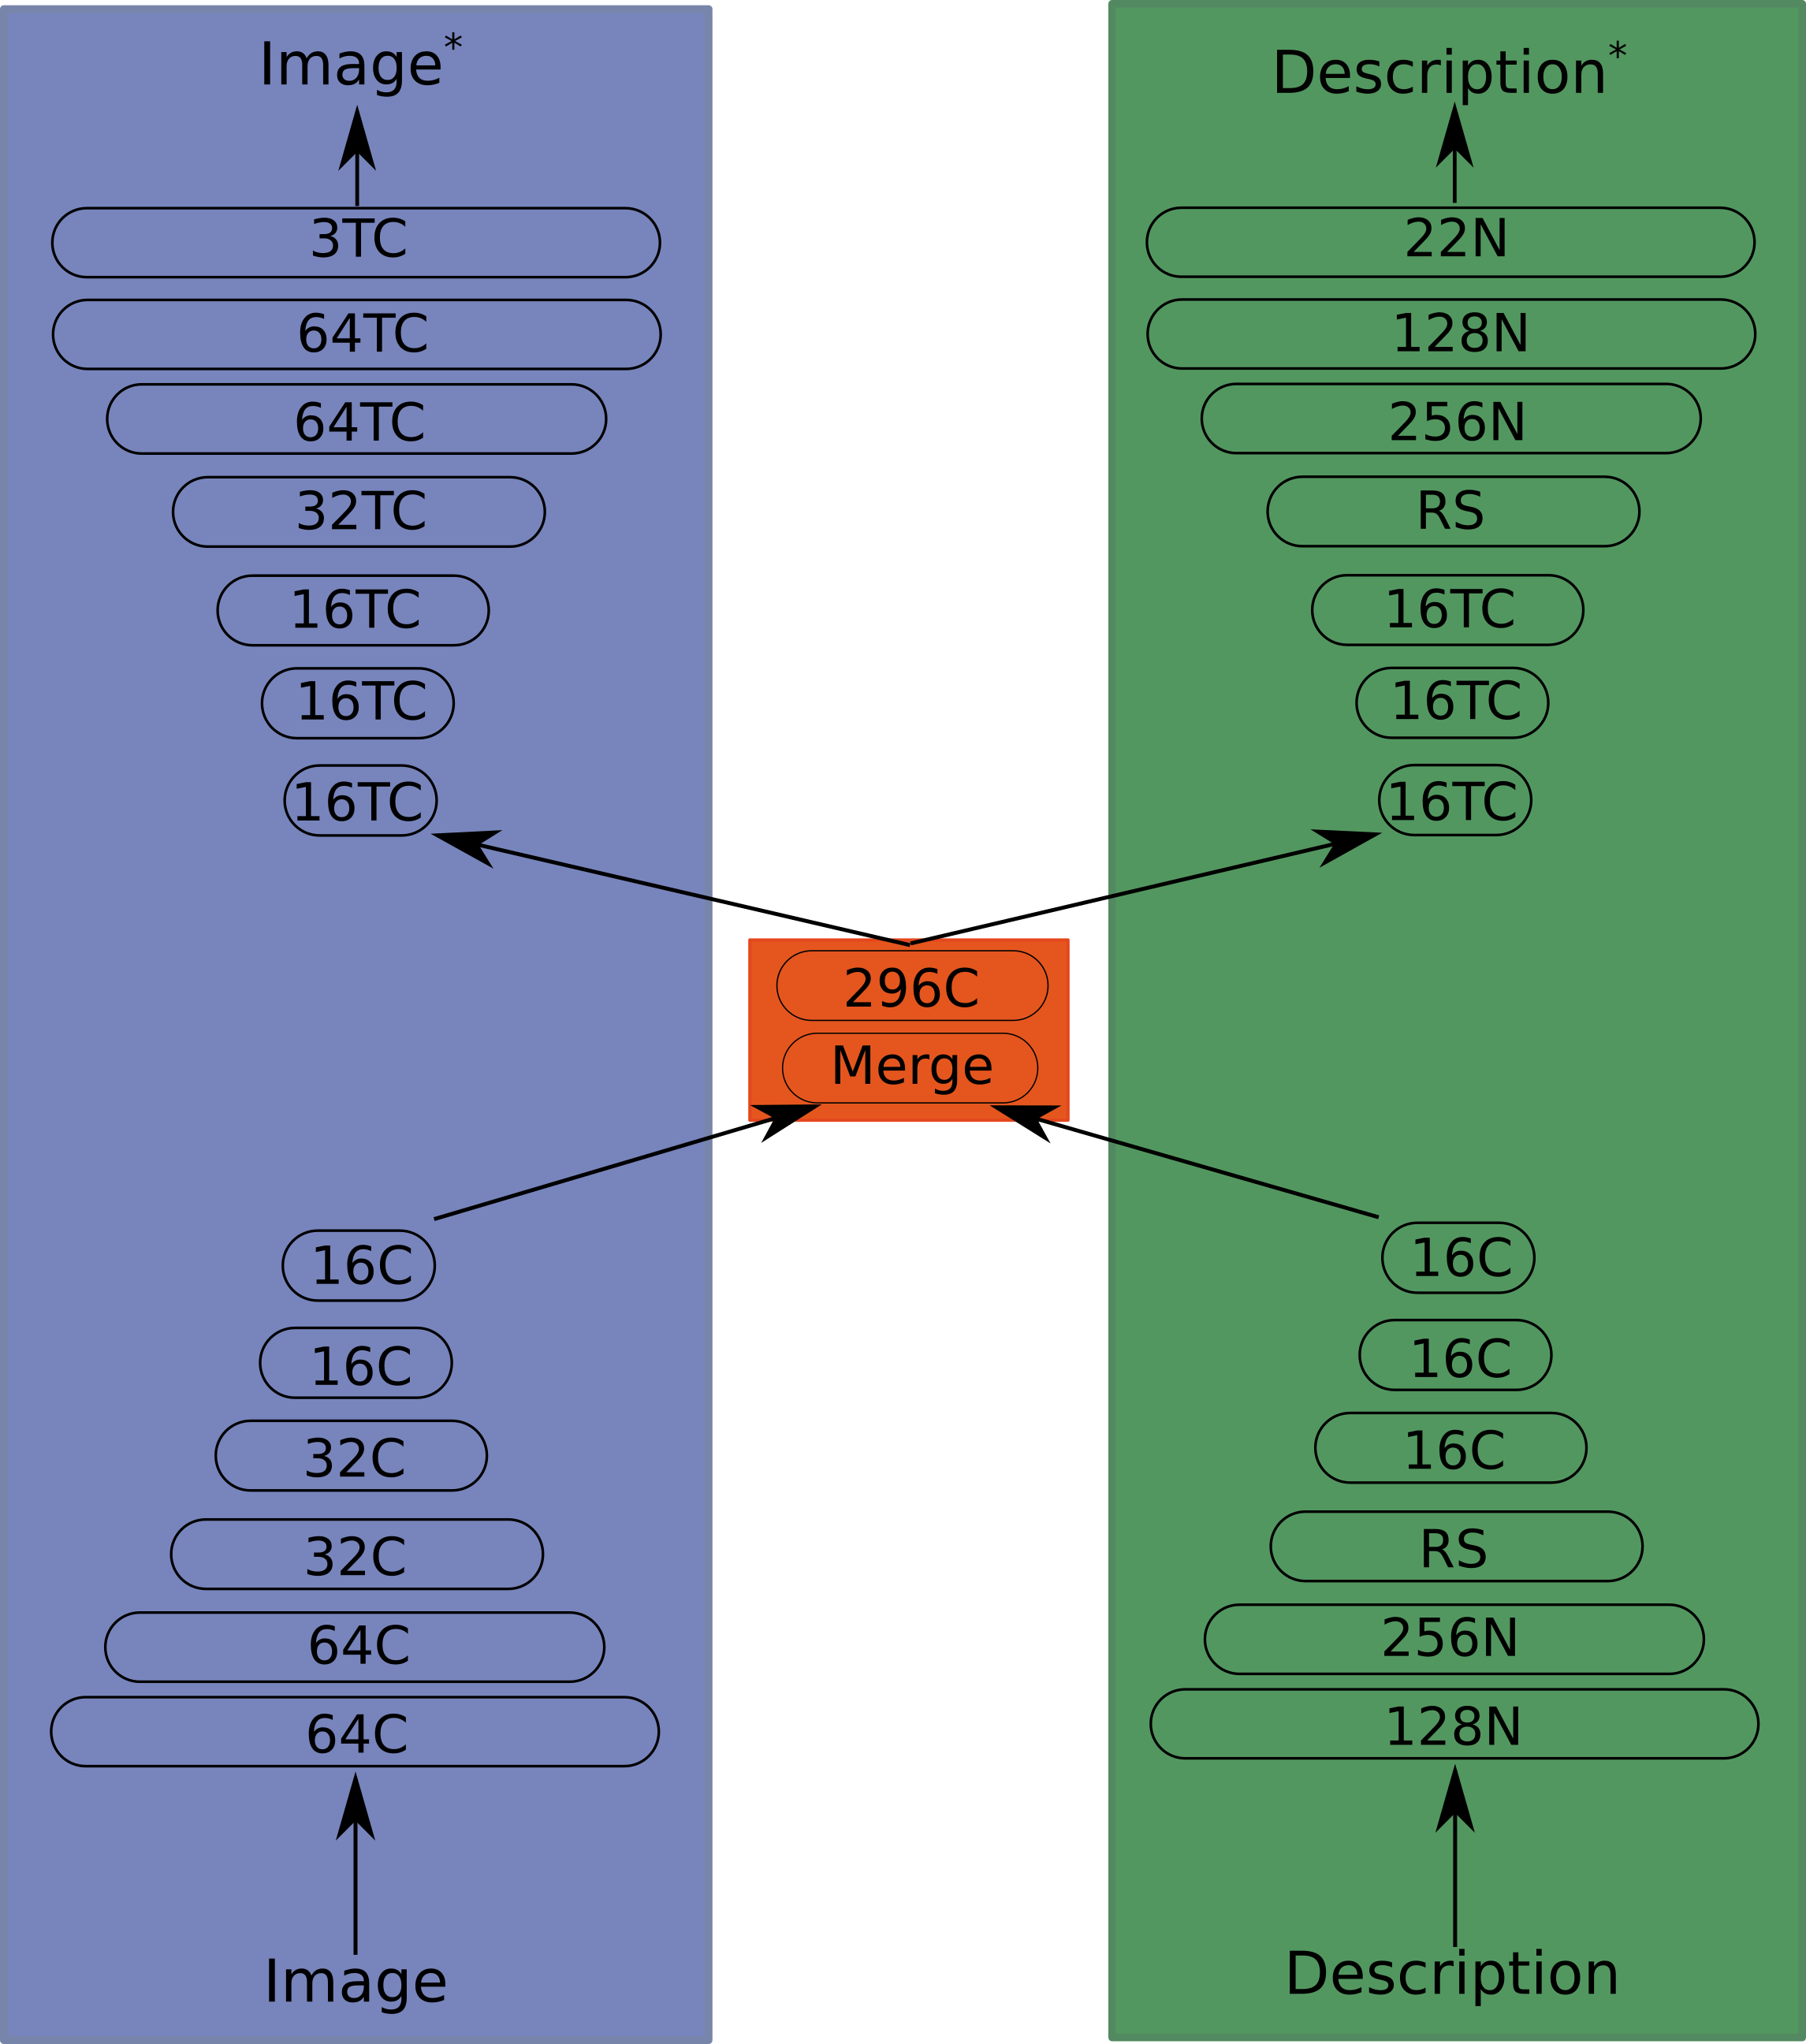
\includegraphics[width=0.75\textwidth]{Figs/shapes/maeArch.png}
\caption{The \ac{MAE} architecture used in this chapters. Layers marked with C are convolution TC, Transposed Convolution, RS, Reshape and N, Dense.}
\label{fig:netArts}
\end{figure}

\autoref{fig:netArts} depicts the \ac{MAE} described in \autoref{tab:Arts_MAE_description}. The blue box shows the portion of the \ac{MAE} which encodes and decodes images, whilst the green portion encodes and decodes the descriptions. The orange box is where the joint representation is formed. Inputs are labelled, Image and Description with their respective outputs being marked with an asterisk.
	


\section{Experiments with the ArtS Dataset}
For each of the following experiments I test the \ac{MAE} in three ways, similarly to the experimental method of \autoref{Chapter4}. Following the protocol of testing in a Bimodal, Image Only and Words Only manner allows me to explore how each of the modalities and their combination, affects the quality of the embedding learnt by the \ac{MAE}. All experiments in this section will utilise the RR training procedure developed in \autoref{Chapter4}.

Due to the complexity of ArtS and the variety of factors which can be explored with it, I perform 5 sets of experiments, each using different subsets of the dataset. All experiments make use of all 3 shapes, but different numbers of colours, sizes and positions will be used. By gradually increasing the complexity of the data, an opportunity to test hypothesis 4 arises, allowing me to explore the effects of transfer learning.

Each experiment is four-fold cross-validated using randomly selected training data and weight initialisations these are referred to as runs A-D.

Each of the 5 experiments builds upon the previous experiments. The first two experiments aim to find the best embedding size for the \ac{MAE}, in order to achieve the best generation results for both images and descriptions. In experiments 1 and 2, I will be directly testing hypothesis 3: \ac{MRL} can be used to learn language as it relates to the visual properties of objects. Whilst also testing the limitations of different sized embeddings for the joint representation of images and descriptions.

Experiments 3 and 4 explore transfer learning, testing hyprothesis 4: \ac{MRL} can be improved through transfer learning. As was seen in the literature review, humans build upon previously learnt skills in order to master new tasks \cite{webb2015mother, fantz1963pattern, reid2017human}, these experiments will determine whether a developmentally inspired learning strategy can aid the \ac{MAE} in learning a high quality, generalisable representation. Particularly, experiments 3 and 4 demonstrate that the representations fulfil the ``semi-supervised learning'' and ``shared factors across tasks'' representation properties put forward by Bengio et al. in \cite{repRev} (Hypothesis 5).

Finally, in experiment 5, I test hypothesis 5: The multimodal representation learnt by the \acp{MAE} exhibits all of the desirable properties of a representation as layed out by Bengio et al. in \cite{repRev}. Experiment 5 ommits a single object from the training data and demonstrates that the neural network is still able to generate images and descriptions of this object by combining the representations of the individual symbols from which the object is constructed. In doing this, I show that the representation learnt by the \ac{MAE} fulfils some of the properties layed out by Bengio et al.

Each experiment introduces more and more complex data in an attempt to find the limits of the \ac{MAE} and its ability to solve the symbol grounding problem. 

\subsection{Experiment 1}
The first experiment utilises 3 colours, 3 positions and 1 size as shown in \autoref{tab:exp1_data}. The aim of this experiment is to find the best size for the embedding layer. I aim to find a number of filters which minimises the reconstruction loss for both the images and descriptions under all testing conditions. Futher to this, I also wish to find an embedding size which allows for the accurate grounding of all words in the dataset. For example, if the \ac{MAE} is given only the word \textsc{Blue} it should generate a \textit{Blue} image, or given the word \textsc{Triangle} an image of a \textit{Triangle}. 

Each shape-colour-size-position combination will be referred to as an object.

For each object, I generate 50 training samples giving a total of 1350 training samples. The validation and testing data consist of 100 samples per object giving 2700 validation and 2700 testing samples.


\begin{table}[ht]
\centering
\begin{tabular}{|c|c|}
\hline
\textbf{Attribute} & \textbf{Description} \\ \hline \hline
\textbf{Shapes} & \textbf{Corners} \\ \hline
Rectangle & 4\\ \hline
Triangle & 3\\ \hline
Circle & 0\\ \hline 

\textbf{Colours} & \textbf{RGB Values}	\\ \hline	
Red & (75,0,0) - (255, 10, 10)\\ \hline
Green  & (0,75,0) - (10, 255, 10)\\ \hline
Blue   & (0,0,75) - (10, 10, 255)\\ \hline


\textbf{Size} & 	\textbf{Length/Radius (pixels)} \\ \hline			  
Big    & 32 - 35  \\ \hline


\textbf{Positions} & \textbf{Object Centre Coordinate}	\\ \hline				  
Centre Left &(22,32)\\ \hline
Centre Centre & (32,32)\\ \hline
Centre Right &(42,32)\\ \hline
				
\end{tabular}
\caption{Experiment 1 data-subset.}
\label{tab:exp1_data} 
\end{table}

\subsubsection{Results}

The affect of increasing the embedding size is mostly to improve the reconstruction error for images, in the Bimodal and Image Only testing conditions as shown by the blue and brown lines in \autoref{fig:graph331} (B). The reconstruction of images from their descriptions is only affected a very small amount by the size of the embedding. With the exception of when the embedding is very small, the description to image reconstruction errors only vary a small amount with respect to the embedding size (red line in \autoref{fig:graph331}). 

\begin{figure}[h]
\centering
\resizebox{0.75\textwidth}{!}{
\begin{tikzpicture}
    \begin{axis}[
     name=plot1,
     axis x line=middle,
     axis y line=middle,
     enlarge y limits=true,
     enlarge x limits=true,
     legend style={at={(0.5,-0.5)}, anchor=north},
     %xmin=0, xmax=2150,
     %ymin=0, ymax=600,
     %width=15cm, height=8cm,     % size of the image
     grid = major,
     grid style={dashed, gray!30},
     ylabel= Total MSE,
     %ytick={0,0.001,0.002,0.003,0.004,0.005,0.006,0.007,0.008,0.009},
     xlabel= (A) Embedding Size,
     %xtick={6,8,10,12,14,16,18,20,22,24,26,28,30,32,34,35,36,37,38,39,40,41,42,43,44,45,46,47,48,49,50,51,52,53,54,55,56},     
	 xlabel near ticks,
	 ylabel near ticks]
         ] 
    ]
    \addplot table[x = size, y = bimodal, col sep = comma]{csvs/331/total331.csv}; 
    \addplot table[x = size, y = words only, col sep = comma]{csvs/331/total331.csv};
    \addplot table[x = size, y = image only, col sep = comma]{csvs/331/total331.csv};    
    \legend{Bimodal, Words Only, Image Only}
    
    \end{axis}
    
    
     \begin{axis}[
     name=plot2,
     at=(plot1.right of south east), 
     anchor=left of south west,
     axis x line=middle,
     axis y line=middle,
     enlarge y limits=true,
     enlarge x limits=true,
     %legend style={at={(1,0.7)}, anchor=north},
     %xmin=0, xmax=2150,
     %ymin=0, ymax=600,
     %width=15cm, height=8cm,     % size of the image
     grid = major,
     grid style={dashed, gray!30},
     ylabel= Image MSE,
     %ytick={0,0.001,0.002,0.003,0.004,0.005,0.006,0.007,0.008,0.009},
     xlabel= (B) Embedding Size,
     %xtick={6,8,10,12,14,16,18,20,22,24,26,28,30,32,34,35,36,37,38,39,40,41,42,43,44,45,46,47,48,49,50,51,52,53,54,55,56},     
     xlabel near ticks,
	 ylabel near ticks]
         ] 
    ]
    \addplot table[x = size, y = bimodal, col sep = comma]{csvs/331/image331.csv}; 
    \addplot table[x = size, y = words only, col sep = comma]{csvs/331/image331.csv};
    \addplot table[x = size, y = image only, col sep = comma]{csvs/331/image331.csv}; 
       
    %\legend{Bimodal, Words Only, Image Only}
    \end{axis}
    
	
    
    \begin{axis}[
     name=plot3,
     at=(plot2.below south west),
     anchor=above north west,
     axis x line=middle,
     axis y line=middle,
     enlarge y limits=true,
     enlarge x limits=true,
     %legend style={at={(1,0.7)}, anchor=north},
     %xmin=0, xmax=2150,
     %ymin=0, ymax=600,
     %width=15cm, height=8cm,     % size of the image
     grid = major,
     grid style={dashed, gray!30},
     ylabel= Description MSE,
     %ytick={0,0.001,0.002,0.003,0.004,0.005,0.006,0.007,0.008,0.009},
     xlabel= (C) Embedding Size,
     %xtick={6,8,10,12,14,16,18,20,22,24,26,28,30,32,34,35,36,37,38,39,40,41,42,43,44,45,46,47,48,49,50,51,52,53,54,55,56},     
     xlabel near ticks,
	 ylabel near ticks]
         ] 
    ]
    \addplot table[x = size, y = bimodal, col sep = comma]{csvs/331/word331.csv}; 
    \addplot table[x = size, y = words only, col sep = comma]{csvs/331/word331.csv};
    \addplot table[x = size, y = image only, col sep = comma]{csvs/331/word331.csv};    
    %\legend{Bimodal, Words Only, Image Only}
    \end{axis}
    

\end{tikzpicture}
}
\caption{Experiment 1: MSE for reconstruction of images and descriptions under different testing conditions. (A) shows the total MSE, (B) shows the MSE of the image output and (C) shows the MSE of the description output.}
\label{fig:graph331}
\end{figure}


\begin{table}[h]
\centering
	\begin{tabular}{|c|c|c|c|}
	\hline
	\textbf{Size} & 	\textbf{Bimodal}	 & 	\textbf{Image Only}	& 	\textbf{Words Only} \\ \hline
8	&	9.17	$\mypm$	0.58	&	9.26	$\mypm$	0.76	&	9.70	$\mypm$	0.67	\\ \hline
40	&	8.33	$\mypm$	0.14	&	7.91	$\mypm$	0.14	&	8.59	$\mypm$	0.13	\\ \hline
72	&	8.09	$\mypm$	0.16	&	7.64	$\mypm$	0.16	&	8.40	$\mypm$	0.14	\\ \hline
104	&	7.69	$\mypm$	0.43	&	7.04	$\mypm$	0.49	&	8.40	$\mypm$	0.24	\\ \hline
136	&	7.14	$\mypm$	0.58	&	6.45	$\mypm$	0.74	&	8.41	$\mypm$	0.16	\\ \hline
168	&	7.01	$\mypm$	0.61	&	6.28	$\mypm$	0.65	&	8.38	$\mypm$	0.17	\\ \hline
200	&	\textbf{6.80}	$\mypm$	0.27	&	\textbf{6.10}	$\mypm$	0.33	&	\textbf{8.30}	$\mypm$	0.17	\\ \hline
232	&	6.97	$\mypm$	0.64	&	6.28	$\mypm$	0.68	&	8.55	$\mypm$	0.05	\\ \hline
264	&	6.92	$\mypm$	0.92	&	6.32	$\mypm$	0.97	&	8.45	$\mypm$	0.24	\\ \hline
296	&	\textbf{6.80}	$\mypm$	1.11	&	6.15	$\mypm$	1.18	&	8.64	$\mypm$	0.27	\\ \hline

	\end{tabular}
\caption{Experiment 1: Total MSE for different embedding sizes for the three testing conditions. An Embedding Size of 200 neurons provides the minimum reconstruction error. (All values are $\times10^{-3}$.)}
\label{tab:res331}
\end{table}

\autoref{tab:res331} allows a closer look at the values of the total error (the sum of image and description reconstruction errors) for the different testing conditions. An embedding size of 200 neurons provides the best total loss in all testing conditions. This performance is matched by an embedding size of 296 neurons in the Bimodal testing condition, however it has a much larger standard deviation as it performs significantly better than the smaller embedding size in the best run but also much worse in the worst run.


From the numerical results presented in \autoref{tab:res331} it is clear that the majority of the error comes from the image output. This is expected as the dimensionality of the images is much larger than the description output (64x64x3 vs 22x1). Notice in particular the scale of the errors in \autoref{fig:graph331}, the image output loss is of a scale $10^{-2}$ compared to the description output which has a scale of $10^{-5}$, three orders of magnitude smaller. 

There is a limit to how good the images reconstructed from descriptions can be as the descriptions do not contain all of the information necessary to perfectly reconstruct the images. This shows up as the difference between image reconstruction in the Image Only testing condition vs the Words Only condition. Put simply, this difference is caused by the standard deviation within the colours and sizes of the objects. 

Whilst the images generated in the Image Only and Bimodal testing conditions have access to exact \ac{RGB} values and exact sizes, the descriptions only contain the name of the colour of the object and can therefore only produce objects with the ``average'' \ac{RGB} values for those words, learnt from the training data. For example, looking at \autoref{tab:exp1_data} it can be seen that the colour \textit{Red} can have RGB values anywhere in the range (75,0,0) - (255, 10, 10).

The standard deviation across the fours runs of the experiment is very low for all embedding sizes, showing that the images generated by the \ac{MAE} are independent of the starting weights and the randomly selected training data from the ArtS dataset. 

\paragraph{Image Generation}

Generating images from full descriptions gives very good quality results as seen in \autoref{fig:331multi}. Here I show images generated with an embedding size of 8 neurons and 200 neurons. From \autoref{tab:res331} it can be seen that 200 gave the best reconstruction error in the Bimodal, Image Only and Words Only testing conditions. However, whilst leading to visible image artificats, the small changes in reconstruction error in the Words Only testing condition are negligble when considering that the semantic information contained in the images is always correct regardless of embedding size. Each description leads to the generation of an image which clearly matches its descriptions, regardless of the embedding size. 

\begin{figure}
\centering
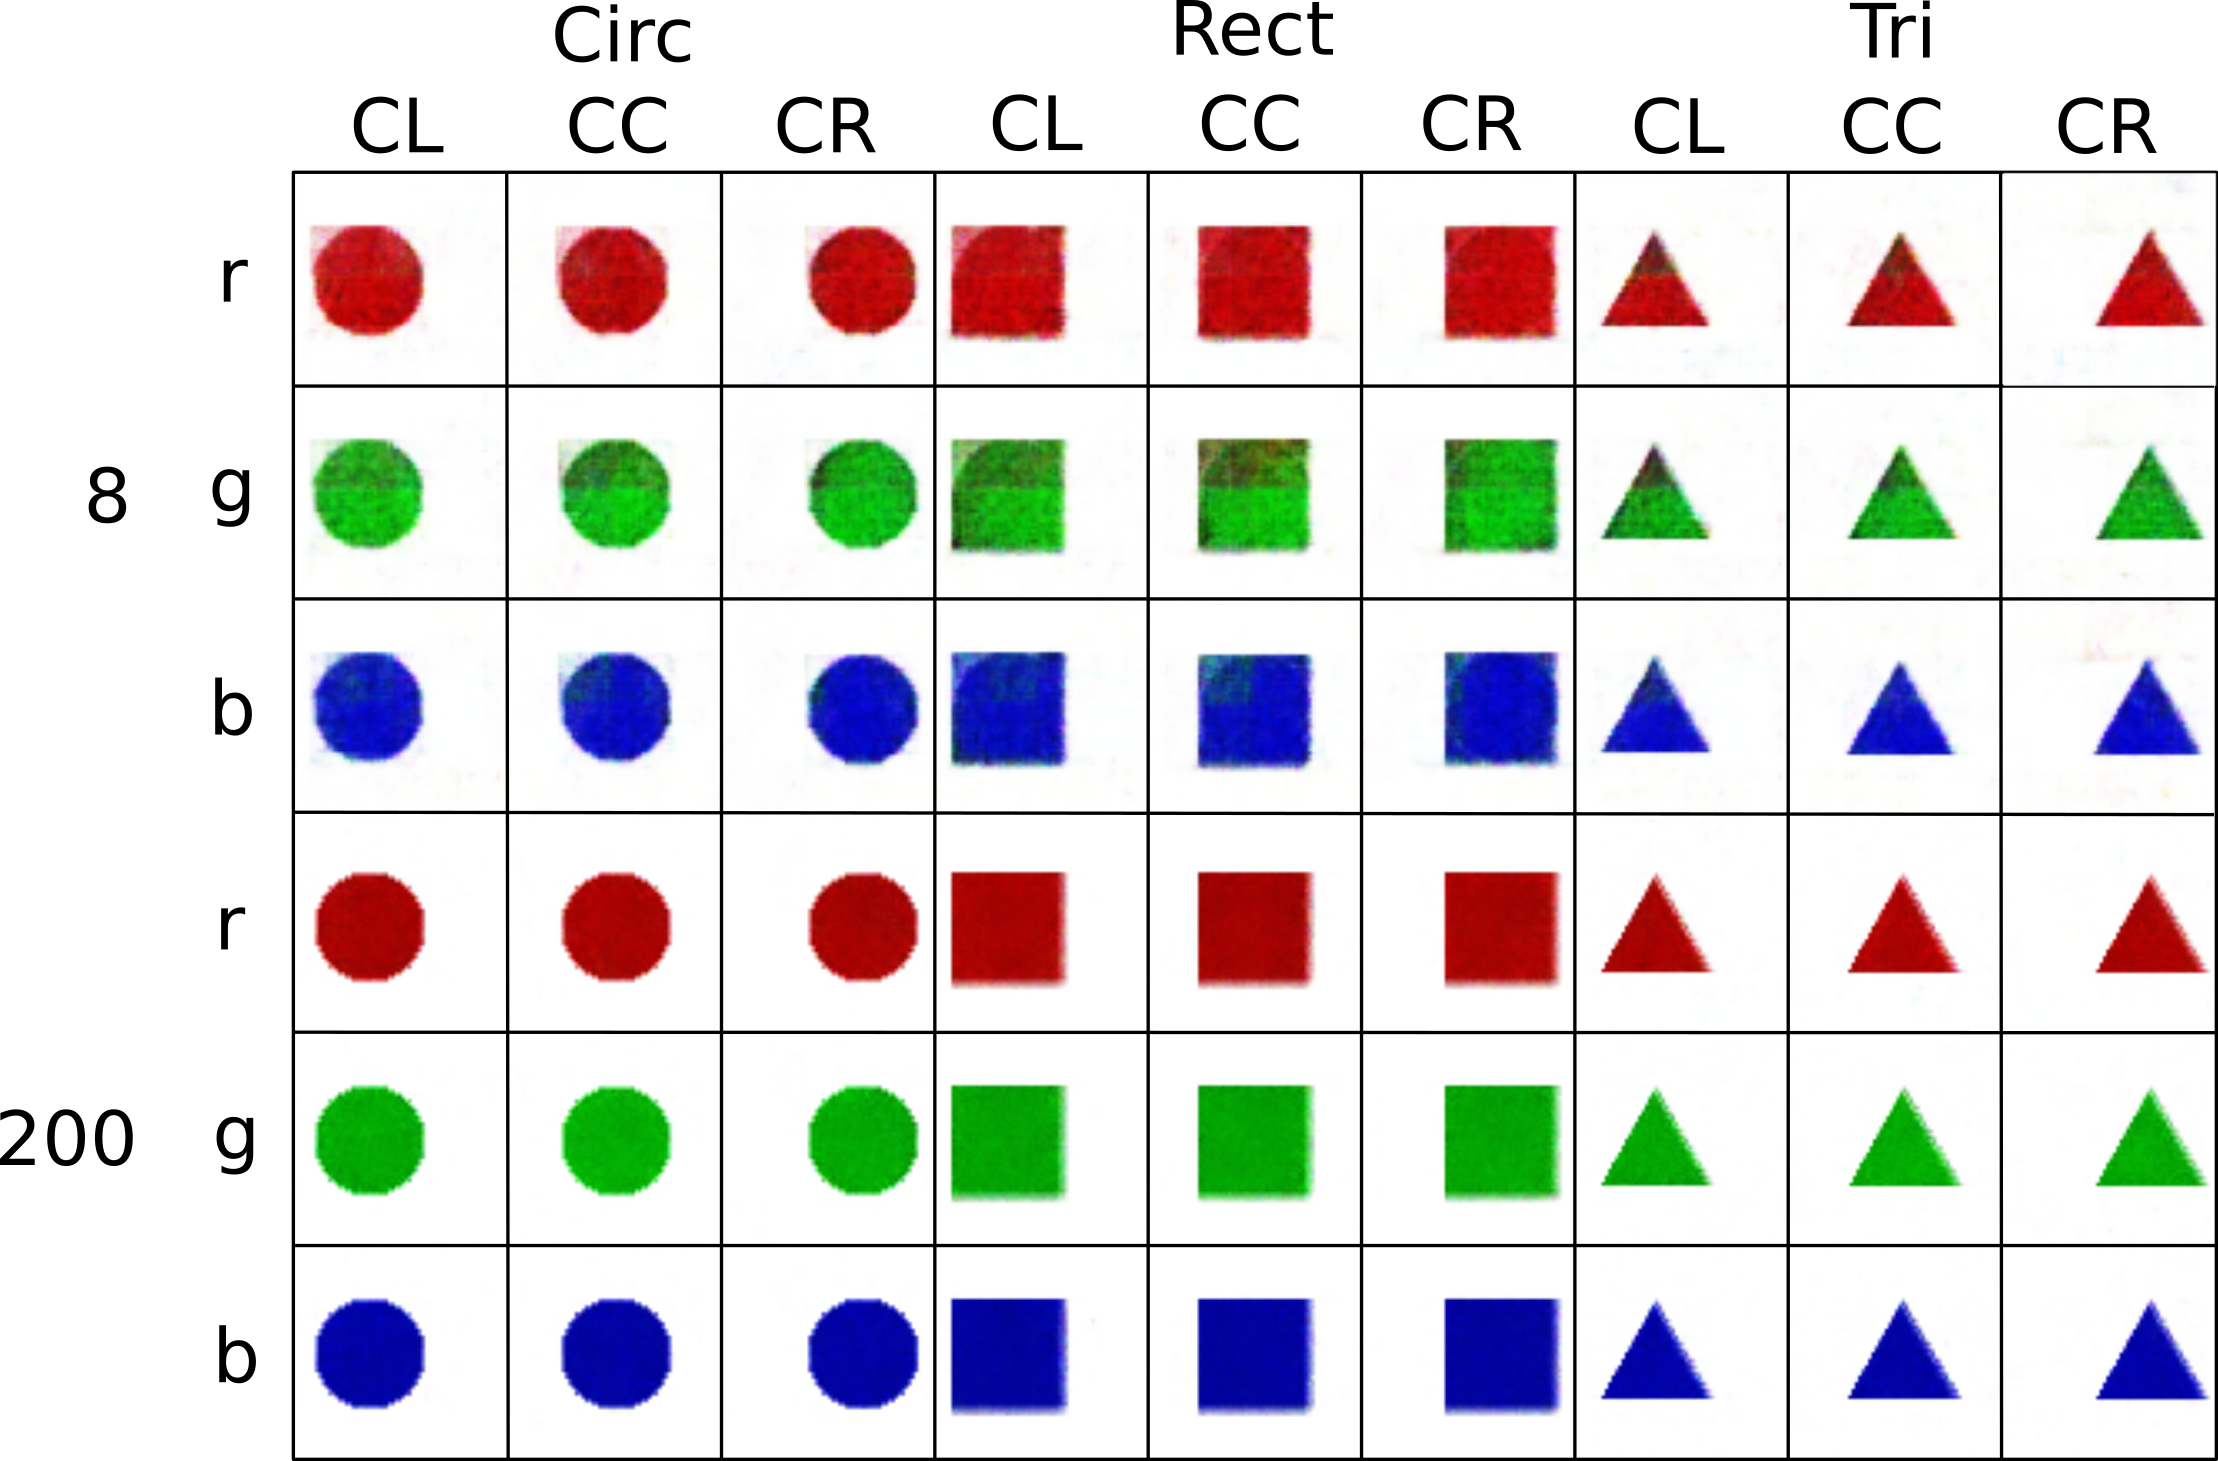
\includegraphics[width=0.625\textwidth]{Figs/shapes/331_8v200.png}
\caption{Images generated from descriptions with an embedding size of 8 or 200 neurons.}
\label{fig:331multi}
\end{figure}

%\begin{figure}[h]
%\centering
%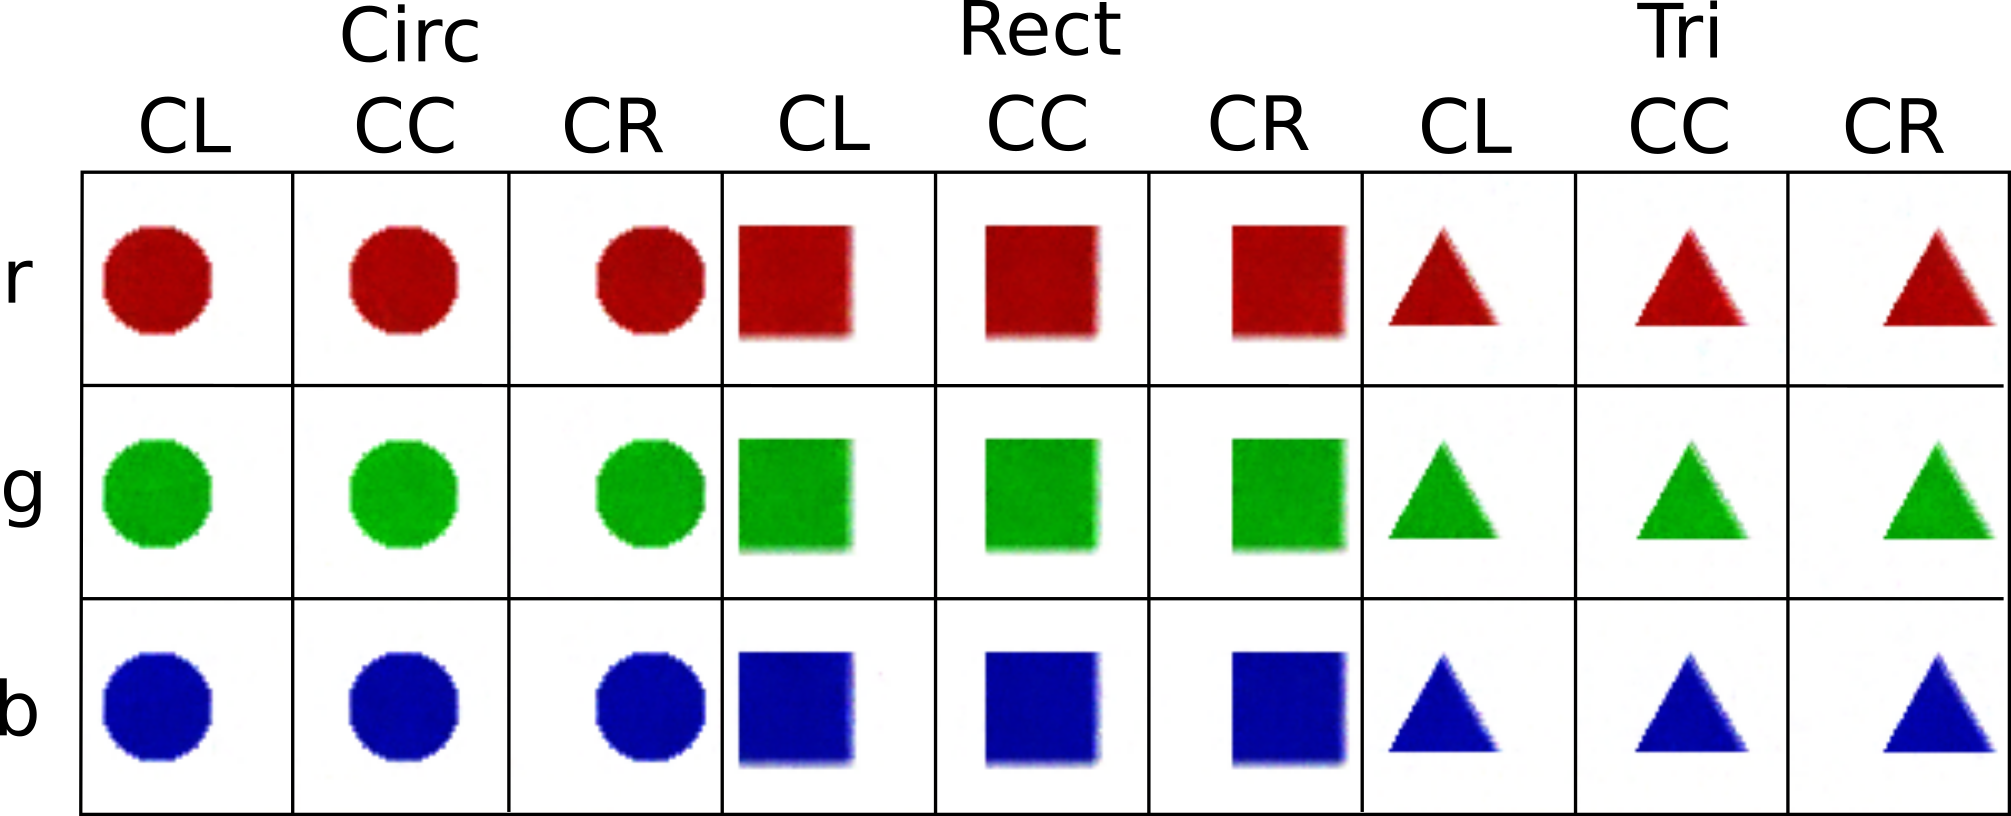
\includegraphics[width=0.75\textwidth]{Figs/shapes/multiword331.png}
%\caption{Experiment 1:  Images generated from descriptions with an embedding size of 200.}
%\label{fig:331multi}
%\end{figure}

Given how well images can be generated from full descriptions, it is unsurpising to see that the \ac{MAE} has been able to correctly ground the meanings of each of the words of the descriptions. In \autoref{fig:331shapes} it can be seen that each shape is correctly generated into an image for most embedding sizes. It is difficult to specify which embedding size grounds the meanings of each word the best as this is subjective. I would suggest that an embedding size of 296 neurons grounds the meanings of individual words the best, this is due to it producing the most solid circle, rectangle and triangle across all four runs, in my opinion. 

\begin{figure}[h]
\centering
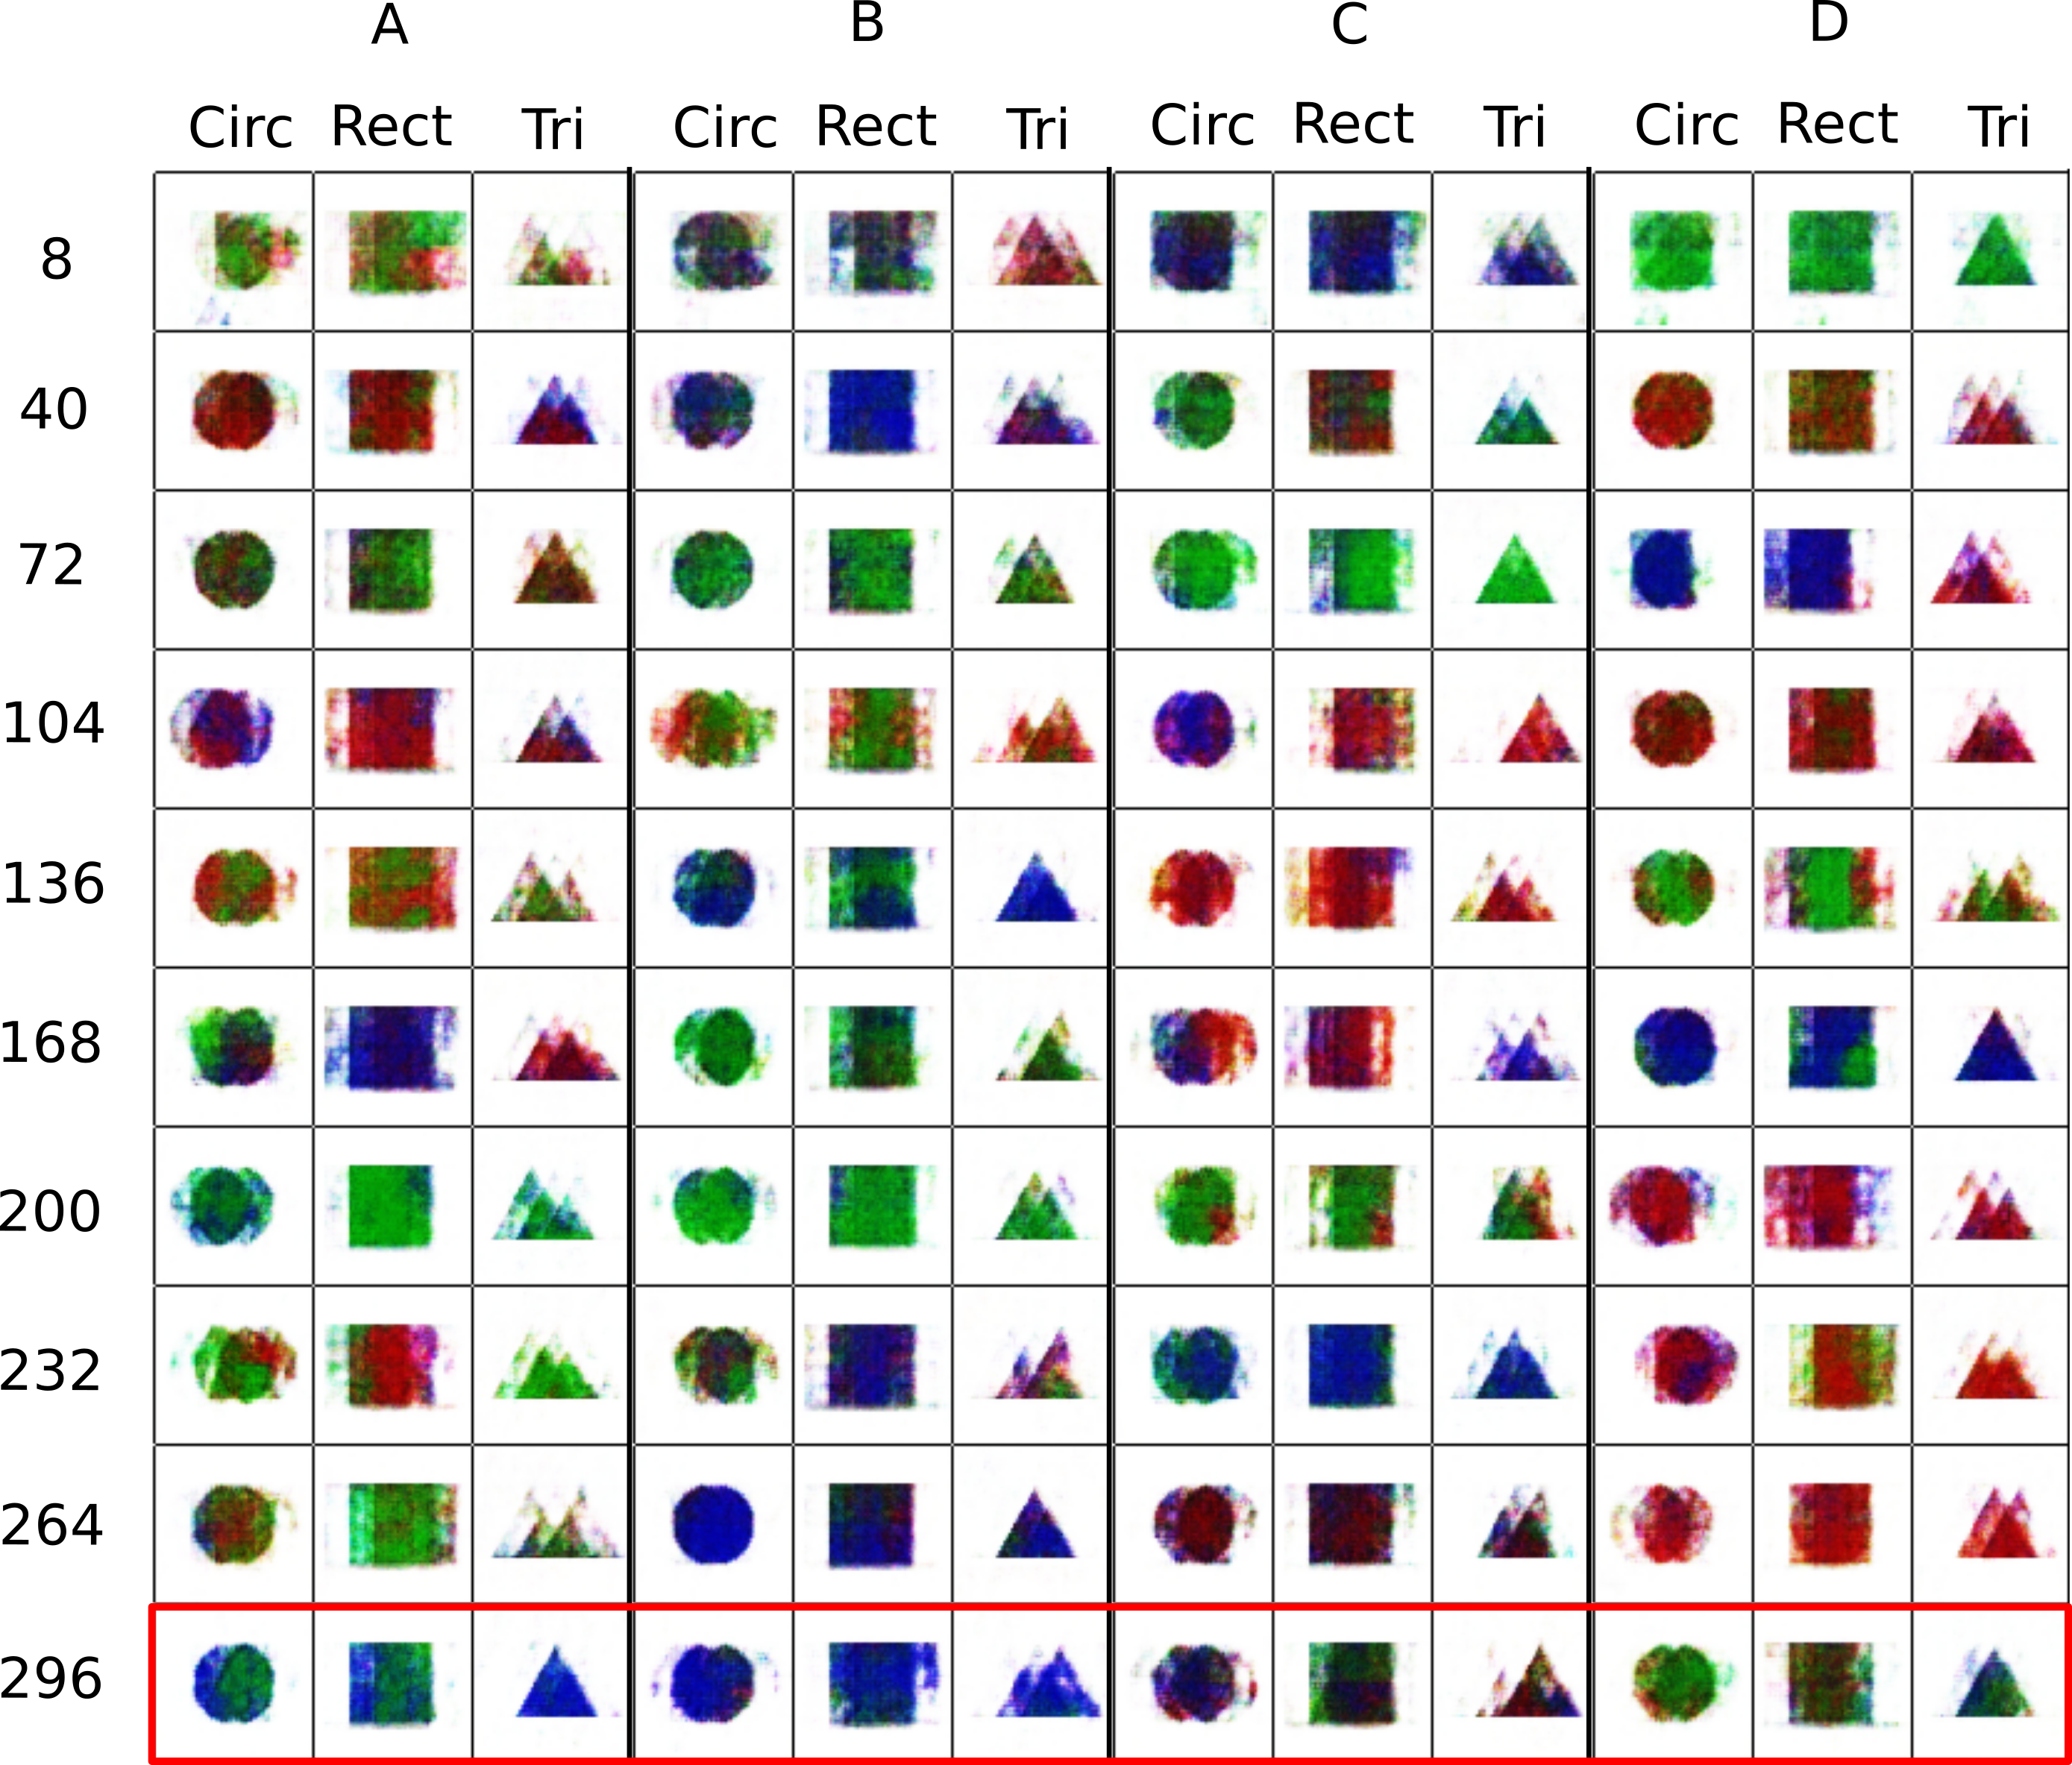
\includegraphics[width=0.75\textwidth]{Figs/shapes/shapes331.png}
\caption{Experiment 1, runs A-D:  Images generated from shape names (\textsc{Circle, Rectangle, Triangle}) for different sizes of embedding.}
\label{fig:331shapes}
\end{figure}

The images generated for every word can be found in the suplimental material. As the colour and position are always  correctly learnt across the four runs, they are not shown in the main text.



\paragraph{Description Accuracy}
The \ac{MAE} gets 100\% accuracy on all descriptions for all testing conditions and all embedding sizes. Accuracy is calculated by counting the number of correctly predicted words and averaging over the entire dataset. For example, given an image described as \textsc{big blue circle left} and the predicted description \textsc{small blue circle left} the accuracy would be 0.75 for that instance as 3 out of 4 words are correctly predicted. A word is considered to be predicted if its neuron's activation is above 0.5. As I am using a sigmoid activation function, the output for each neuron is always between 0 and 1.


\subsubsection{Discussion}
The results of experiment 1 show that the \ac{MAE} is capable of preforming symbol grounding on this subset of the ArtS dataset. However, it is difficult to make any conclusions about which embedding size gave the best results. Whilst 200 neurons gave the lowest reconstruction error in all testing conditions (see \autoref{tab:res331}), it did not do the best job of grounding the meanings of each word in the descritptions (see \autoref{fig:331shapes}). 

This experiment has already proven hypothesis 3: \ac{MRL} can be used to learn language as it relates to the visual properties of objects. However, I wish to test this hypothesis on more complex data. As such, in the next experiment, I will observe how embedding size affects the reconstruction error and symbol grounding of the \ac{MAE} when a larger variety of sizes for the objects in the images are available.


\newpage
\subsection{Experiment 2}
I will now explore how adding more variety to the data affects the quality of reconstruction. To that end, two new sizes of object are added as seen in \autoref{tab:exp2_data}. 

\begin{table}[ht]
\centering
\begin{tabular}{|c|c|}
\hline
\textbf{Attribute} & \textbf{Description} \\ \hline \hline
\textbf{Shapes} & \textbf{Corners} \\ \hline
Rectangle & 4\\ \hline
Triangle & 3\\ \hline
Circle & 0\\ \hline 

\textbf{Colours} & \textbf{RGB Values}	\\ \hline	
Red & (75,0,0) - (255, 10, 10)\\ \hline
Green  & (0,75,0) - (10, 255, 10)\\ \hline
Blue   & (0,0,75) - (10, 10, 255)\\ \hline


\textbf{Sizes} & 	\textbf{Length/Radius (pixels)} \\ \hline			  
Big    & 32 - 35  \\ \hline
Medium & 22 - 25 \\ \hline
Small  & 12 - 15 \\ \hline 

\textbf{Positions} & \textbf{Object Centre Coordinate}	\\ \hline					  
Centre Left &(22,32)\\ \hline
Centre Centre & (32,32)\\ \hline
Centre Right &(42,32)\\ \hline				
\end{tabular}
\caption{Experiment 2 data-subset.}
\label{tab:exp2_data} 
\end{table}



\subsubsection{Results}
\begin{figure}
\centering
\resizebox{0.75\textwidth}{!}{
\begin{tikzpicture}
    \begin{axis}[
     name=plot1,
     axis x line=middle,
     axis y line=middle,
     enlarge y limits=true,
     enlarge x limits=true,
     legend style={at={(0.5,-0.5)}, anchor=north},
     %xmin=0, xmax=2150,
     %ymin=0, ymax=600,
     %width=15cm, height=8cm,     % size of the image
     grid = major,
     grid style={dashed, gray!30},
     ylabel= Total MSE,
     %ytick={0,0.001,0.002,0.003,0.004,0.005,0.006,0.007,0.008,0.009},
     xlabel= (A) Embedding Size,
     %xtick={6,8,10,12,14,16,18,20,22,24,26,28,30,32,34,35,36,37,38,39,40,41,42,43,44,45,46,47,48,49,50,51,52,53,54,55,56},     
	 xlabel near ticks,
	 ylabel near ticks]
         ] 
    ]
    \addplot table[x = size, y = bimodal, col sep = comma]{csvs/333/total333.csv}; 
    \addplot table[x = size, y = words only, col sep = comma]{csvs/333/total333.csv};
    \addplot table[x = size, y = image only, col sep = comma]{csvs/333/total333.csv};    
    \legend{Bimodal, Words Only, Image Only}
    
    \end{axis}
    
    
     \begin{axis}[
     name=plot2,
     at=(plot1.right of south east), 
     anchor=left of south west,
     axis x line=middle,
     axis y line=middle,
     enlarge y limits=true,
     enlarge x limits=true,
     %legend style={at={(1,0.7)}, anchor=north},
     %xmin=0, xmax=2150,
     %ymin=0, ymax=600,
     %width=15cm, height=8cm,     % size of the image
     grid = major,
     grid style={dashed, gray!30},
     ylabel= Image MSE,
     %ytick={0,0.001,0.002,0.003,0.004,0.005,0.006,0.007,0.008,0.009},
     xlabel= (B) Embedding Size,
     %xtick={6,8,10,12,14,16,18,20,22,24,26,28,30,32,34,35,36,37,38,39,40,41,42,43,44,45,46,47,48,49,50,51,52,53,54,55,56},     
     xlabel near ticks,
	 ylabel near ticks]
         ] 
    ]
    \addplot table[x = size, y = bimodal, col sep = comma]{csvs/333/image333.csv}; 
    \addplot table[x = size, y = words only, col sep = comma]{csvs/333/image333.csv};
    \addplot table[x = size, y = image only, col sep = comma]{csvs/333/image333.csv}; 
       
    %\legend{Bimodal, Words Only, Image Only}
    \end{axis}
    
	
    
    \begin{axis}[
     name=plot3,
     at=(plot2.below south west),
     anchor=above north west,
     axis x line=middle,
     axis y line=middle,
     enlarge y limits=true,
     enlarge x limits=true,
     %legend style={at={(1,0.7)}, anchor=north},
     %xmin=0, xmax=2150,
     %ymin=0, ymax=600,
     %width=15cm, height=8cm,     % size of the image
     grid = major,
     grid style={dashed, gray!30},
     ylabel= Desciption MSE,
     %ytick={0,0.001,0.002,0.003,0.004,0.005,0.006,0.007,0.008,0.009},
     xlabel= (C) Embedding Size,
     %xtick={6,8,10,12,14,16,18,20,22,24,26,28,30,32,34,35,36,37,38,39,40,41,42,43,44,45,46,47,48,49,50,51,52,53,54,55,56},     
     xlabel near ticks,
	 ylabel near ticks]
         ] 
    ]
    \addplot table[x = size, y = bimodal, col sep = comma]{csvs/333/word333.csv}; 
    \addplot table[x = size, y = words only, col sep = comma]{csvs/333/word333.csv};
    \addplot table[x = size, y = image only, col sep = comma]{csvs/333/word333.csv};    
    %\legend{Bimodal, Words Only, Image Only}
    \end{axis}
    

\end{tikzpicture}
}
\caption{Experiment 2: MSE for reconstruction of images and descriptions under different testing conditions. (A) shows the total MSE, (B) shows the MSE of the image output and (C) shows the MSE of the description output.}
\label{fig:graph333}
\end{figure}

Once again, it can be seen that the majority of error comes from the image reconstruction loss by comparing the scales of \autoref{fig:graph333} (B) and (C). The description reconstruction error is larger and less stable with respect to the embedding size than in experiment 1. However it still remains very small with a scale of $10^{-4}$ vs $10^{-5}$. As words are considered to be predicted if their neuron has an activation over 0.5 (maximum activation is 1 as they are sigmoid neurons), this small change in error does not have a significant effect on the accuracy of the generated descriptions.

Interestingly, it can be seen that increasing the embedding size seems to have a positive effect on image reconstruction error under all testing conditions, though this is not a large improvement in the Words Only testing condition. \autoref{tab:res333} highlights this, with the best total error occuring for an embedding size of 296 neurons in all three testing conditions. 
Comparing this to the results of experiment 1, where 200 neurons was the best embedding size with respect to reconstruction error, it is possible that as the data becomes more complex, the extra neurons allow for better represention of the multimodal data. In future, the addition of more neurons should be considered, however as \acp{ANN} take a considerable amount of time to train, I was unable to explore larger embedding sizes in this thesis.

\begin{table}
\centering
	\begin{tabular}{|c|c|c|c|}
	\hline
	\textbf{Size} & 	\textbf{Bimodal} & 	\textbf{Image Only} 	& 	\textbf{Words Only} \\ \hline
8	&	6.65	$\mypm$	0.20	&	6.68	$\mypm$	0.30	&	7.37	$\mypm$	0.30	\\ \hline
40	&	5.38	$\mypm$	0.10	&	5.27	$\mypm$	0.30	&	5.66	$\mypm$	0.10	\\ \hline
72	&	5.57	$\mypm$	0.50	&	6.67	$\mypm$	1.90	&	5.90	$\mypm$	0.50	\\ \hline
104	&	5.04	$\mypm$	0.20	&	4.69	$\mypm$	0.20	&	5.52	$\mypm$	0.20	\\ \hline
136	&	4.89	$\mypm$	0.20	&	4.57	$\mypm$	0.20	&	5.53	$\mypm$	0.10	\\ \hline
168	&	4.91	$\mypm$	0.20	&	4.50	$\mypm$	0.20	&	5.51	$\mypm$	0.10	\\ \hline
200	&	4.70	$\mypm$	0.20	&	4.60	$\mypm$	0.70	&	5.47	$\mypm$	0.10	\\ \hline
232	&	4.91	$\mypm$	0.30	&	4.53	$\mypm$	0.30	&	5.66	$\mypm$	0.20	\\ \hline
264	&	4.64	$\mypm$	0.20	&	4.28	$\mypm$	0.20	&	5.46	$\mypm$	0.10	\\ \hline
296	&	\textbf{4.41}	$\mypm$	0.10	&	\textbf{4.19}	$\mypm$	0.30	&	\textbf{5.44}	$\mypm$	0.10	\\ \hline

	\end{tabular}
\caption{Experiment 2:  Total MSE for different embedding sizes. An Embedding Size of 296 neurons provides the minimum reconstruction error. (All values are $\times10^{-3}$.)}
\label{tab:res333}
\end{table}


\paragraph{Image Generation}

\begin{figure}[h]
\centering
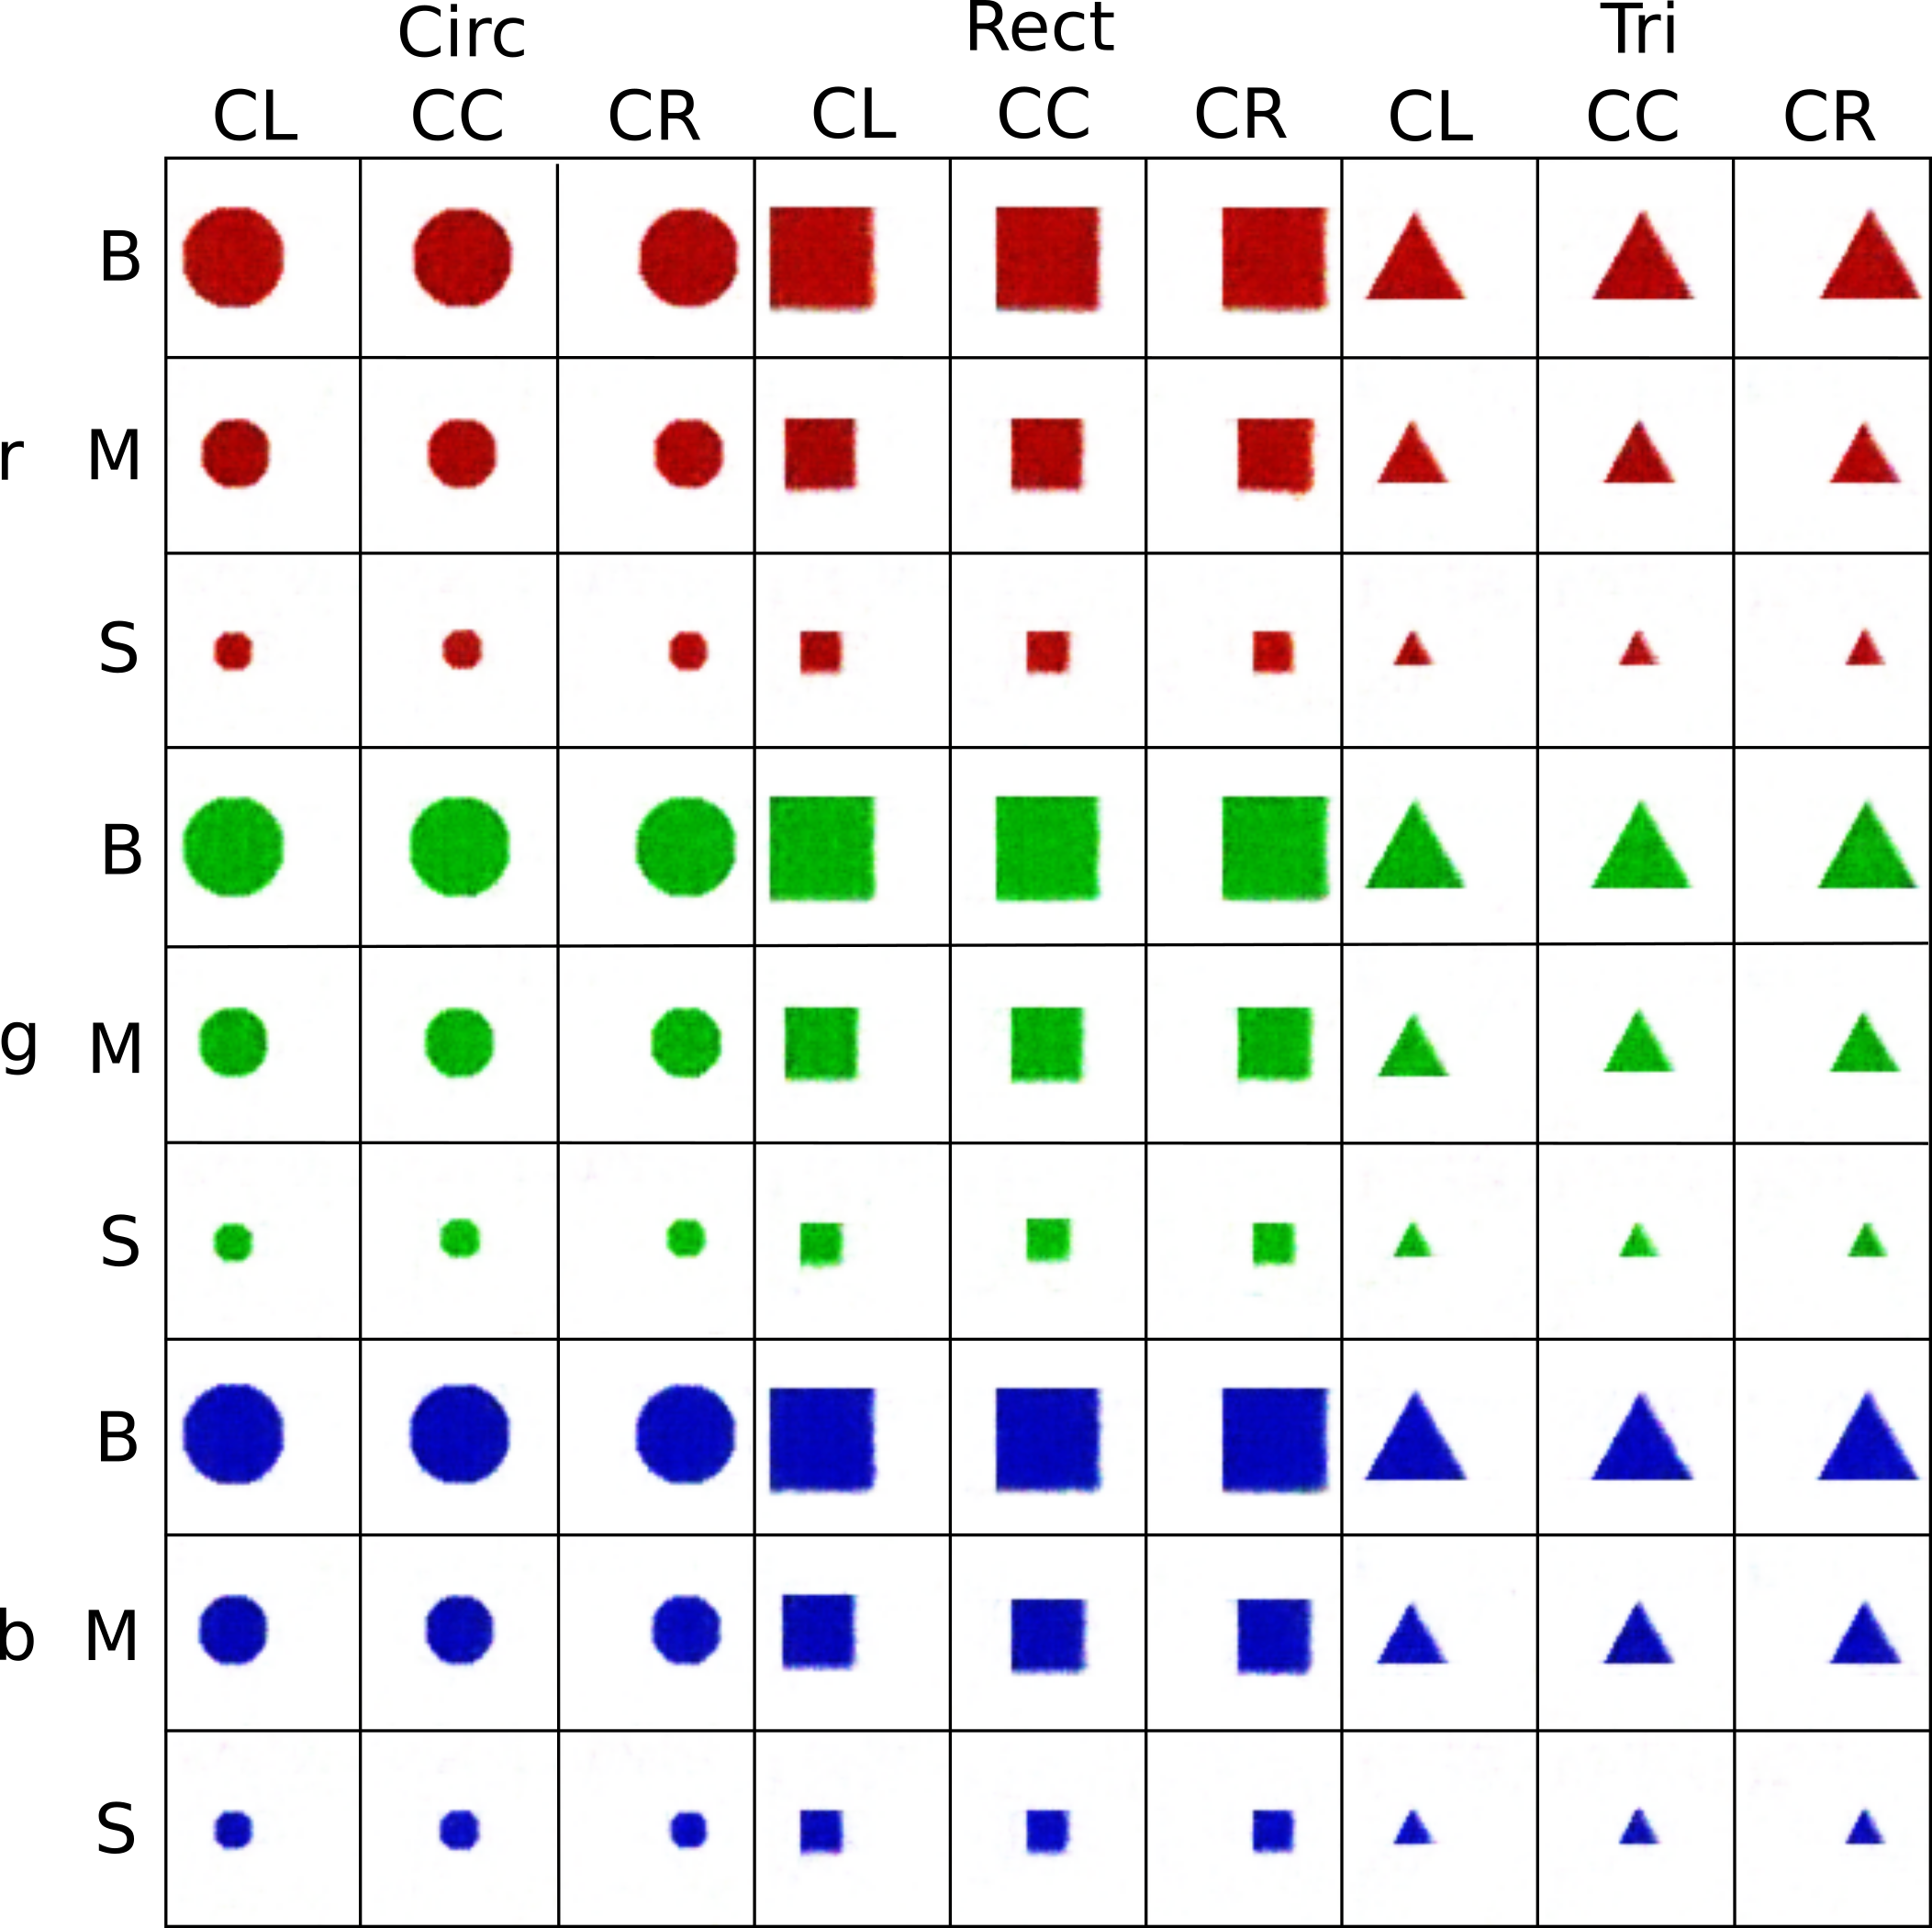
\includegraphics[width=0.5\textwidth]{Figs/shapes/multiword333.png}
\caption{Experiment 2: Images generated from descriptions with an embedding size of 296 neurons. CL, CC and CR are centre-left, centre-centre and centre-right, respectively.}
\label{fig:333multi}
\end{figure}

Generating images from full descriptions remains effective as seen in \autoref{fig:333multi}.
With the addition of the extra sizes, generation of images from a single word has become significantly poorer. However, it is still clear that at least some of the words have been succefully grounded. Particularly, the meaning of colours and positions are correctly learnt, with images of distinct colours and positions being generated as seen in \autoref{fig:333single}. 

\begin{figure}[h]
\centering
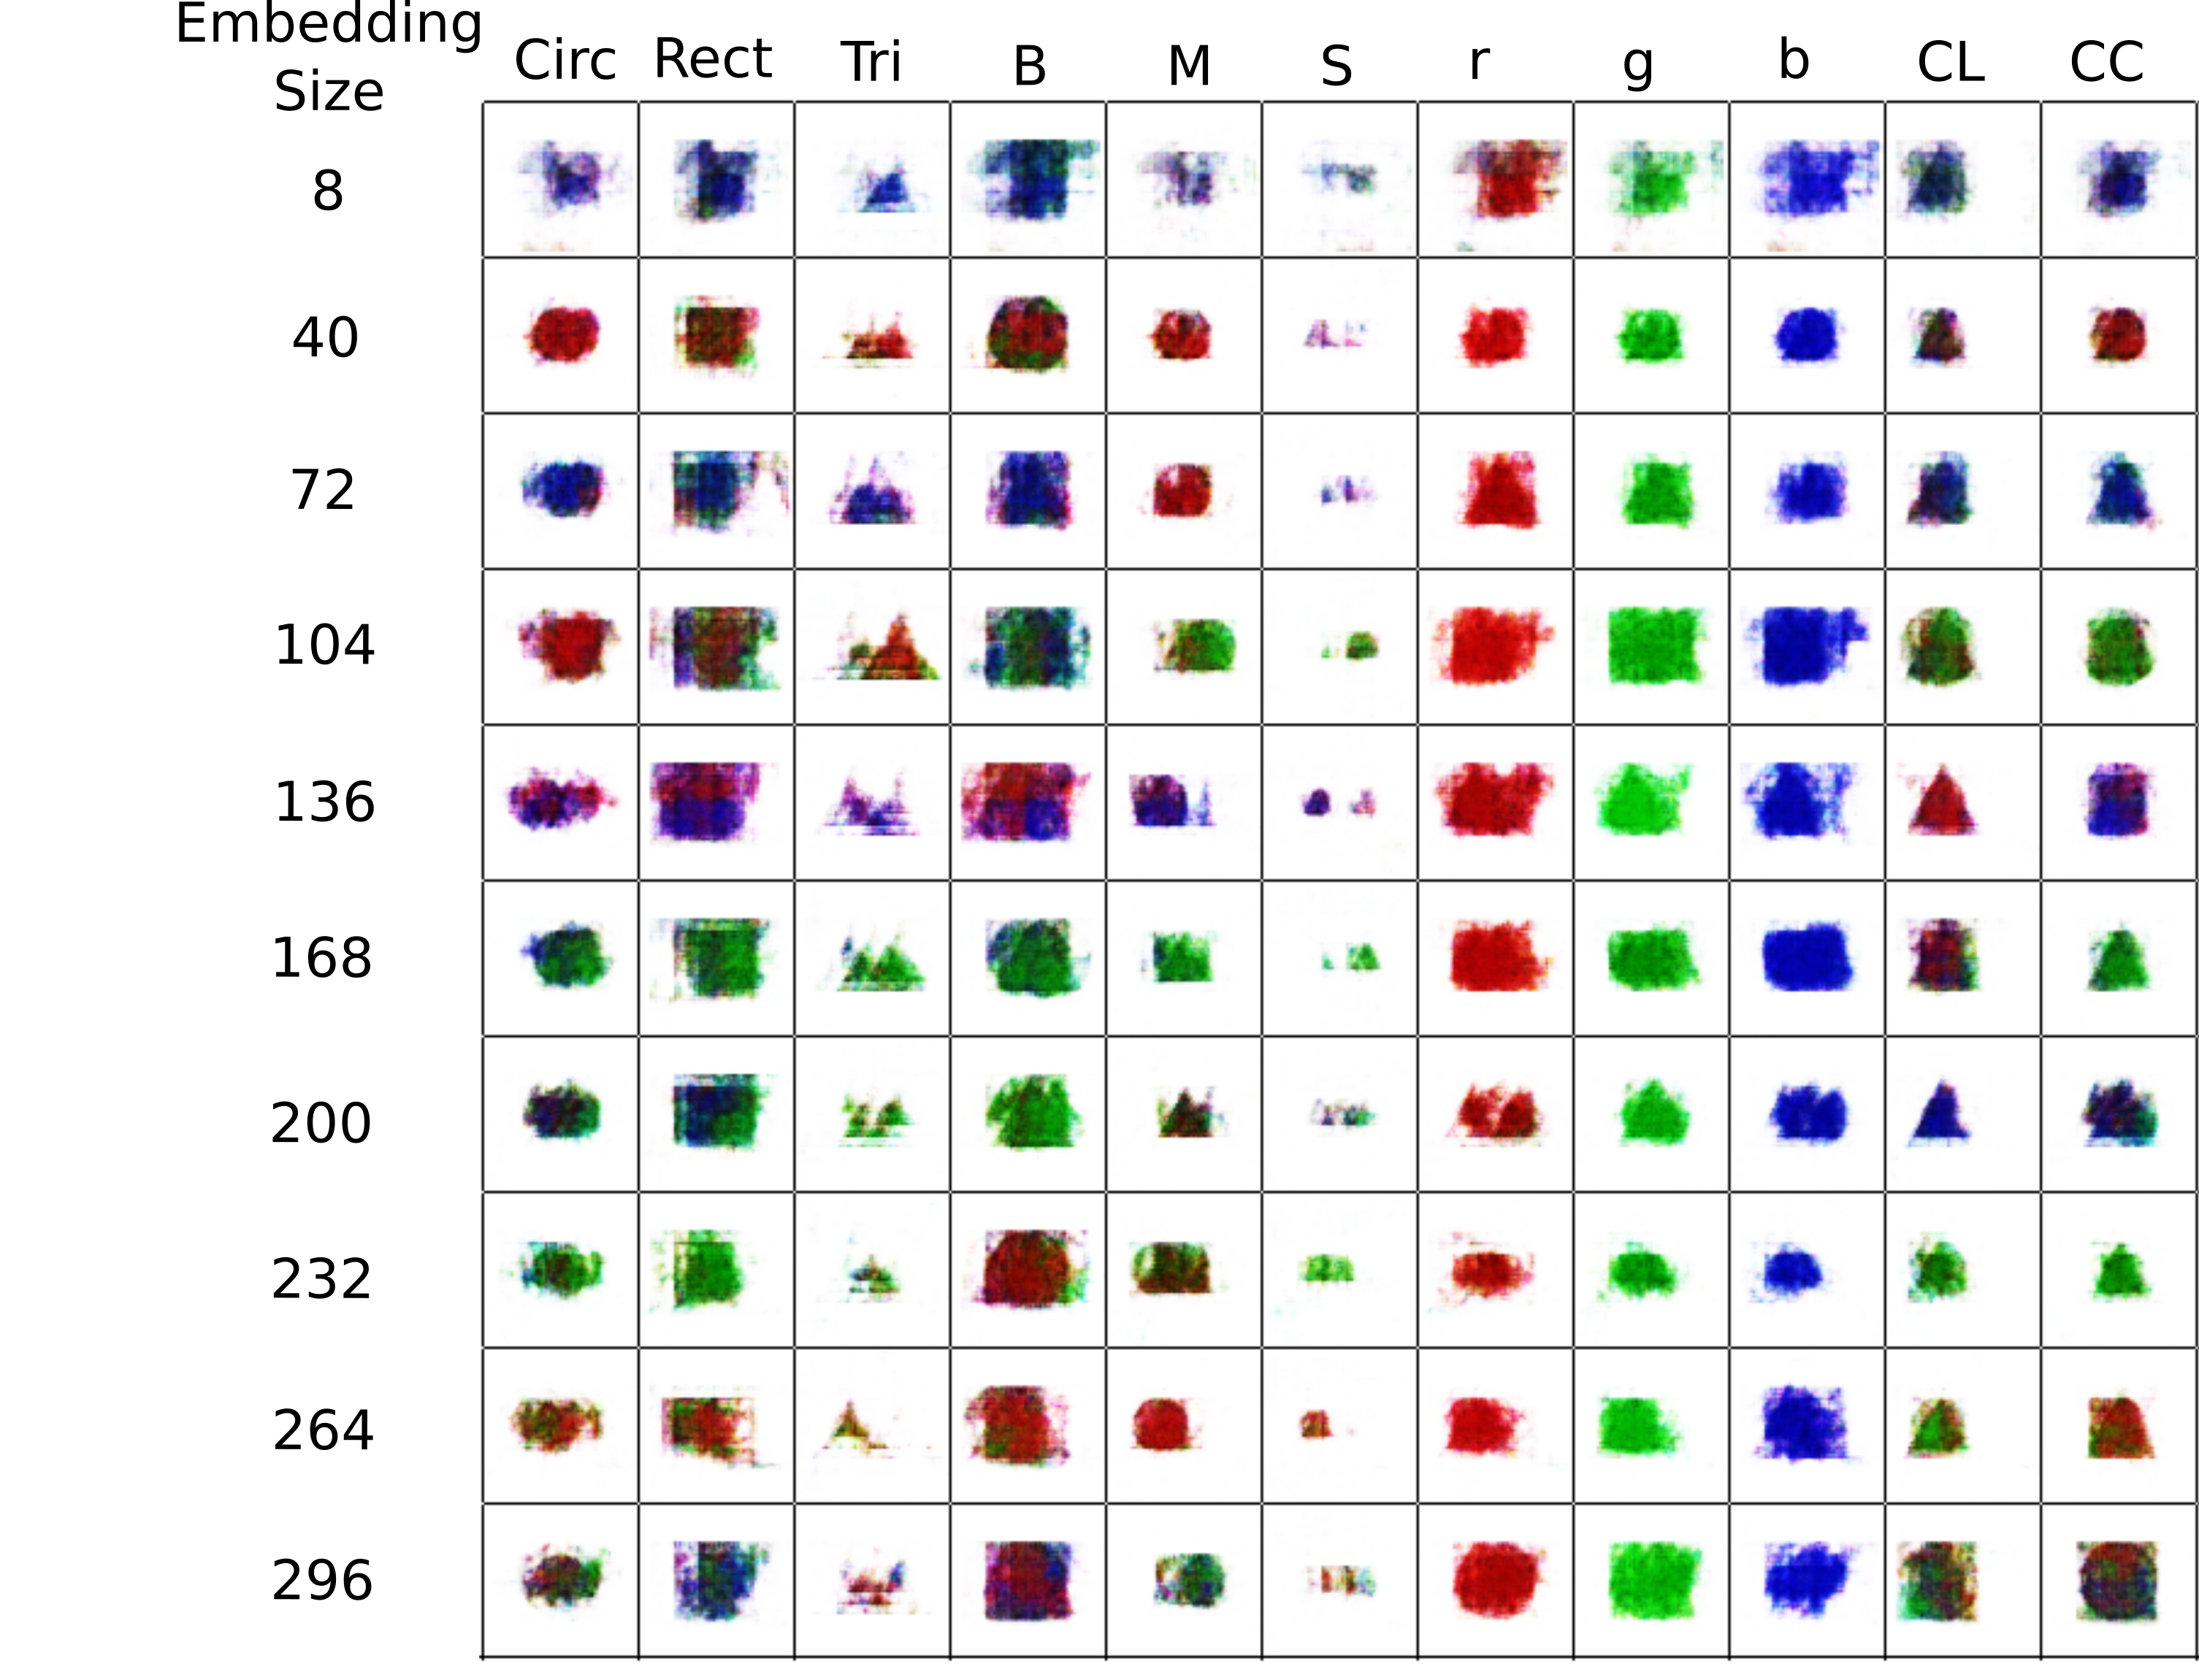
\includegraphics[width=0.75\textwidth]{Figs/shapes/singlelabel333A.png}
\caption{Experiment 2 run A: Images generated of each word (\textsc{Circle, Rectangle, Triangle, Big, Medium, Small, Red, Green, Blue, Centre-Left, Centre-Centre, Centre-Right}) for different embedding sizes.}
\label{fig:333single}
\end{figure} 

There is also a clear releationship between the three sizes, shown by the generation of the most coloured pixels for the word \textsc{Big}, fewer for \textsc{Medium} and the least for \textsc{Small}.


The quality of the shapes being generated from the words \textsc{Circle}, \textsc{Rectangle} and \textsc{Triangle} has suffered the most. However, there is a clear difference between the three shapes and they do show properties of the shapes they are supposed to be. The \textsc{Circle} is more round than either of the other shapes. The \textsc{Rectangle} has approxiamtely 4 sides at right angles to one and other, though it shows significantly more blur than in experiment 1. The \textsc{Triangle} appears triangular, however, for most embedding sizes there appear to be multiple triangles being drawn, this could signify a confusion about where to draw the triangle. I reason that this is the case as in \autoref{fig:2word333} the triangle is significantly more solid when a position is specified. 


\begin{figure}[h]
\centering
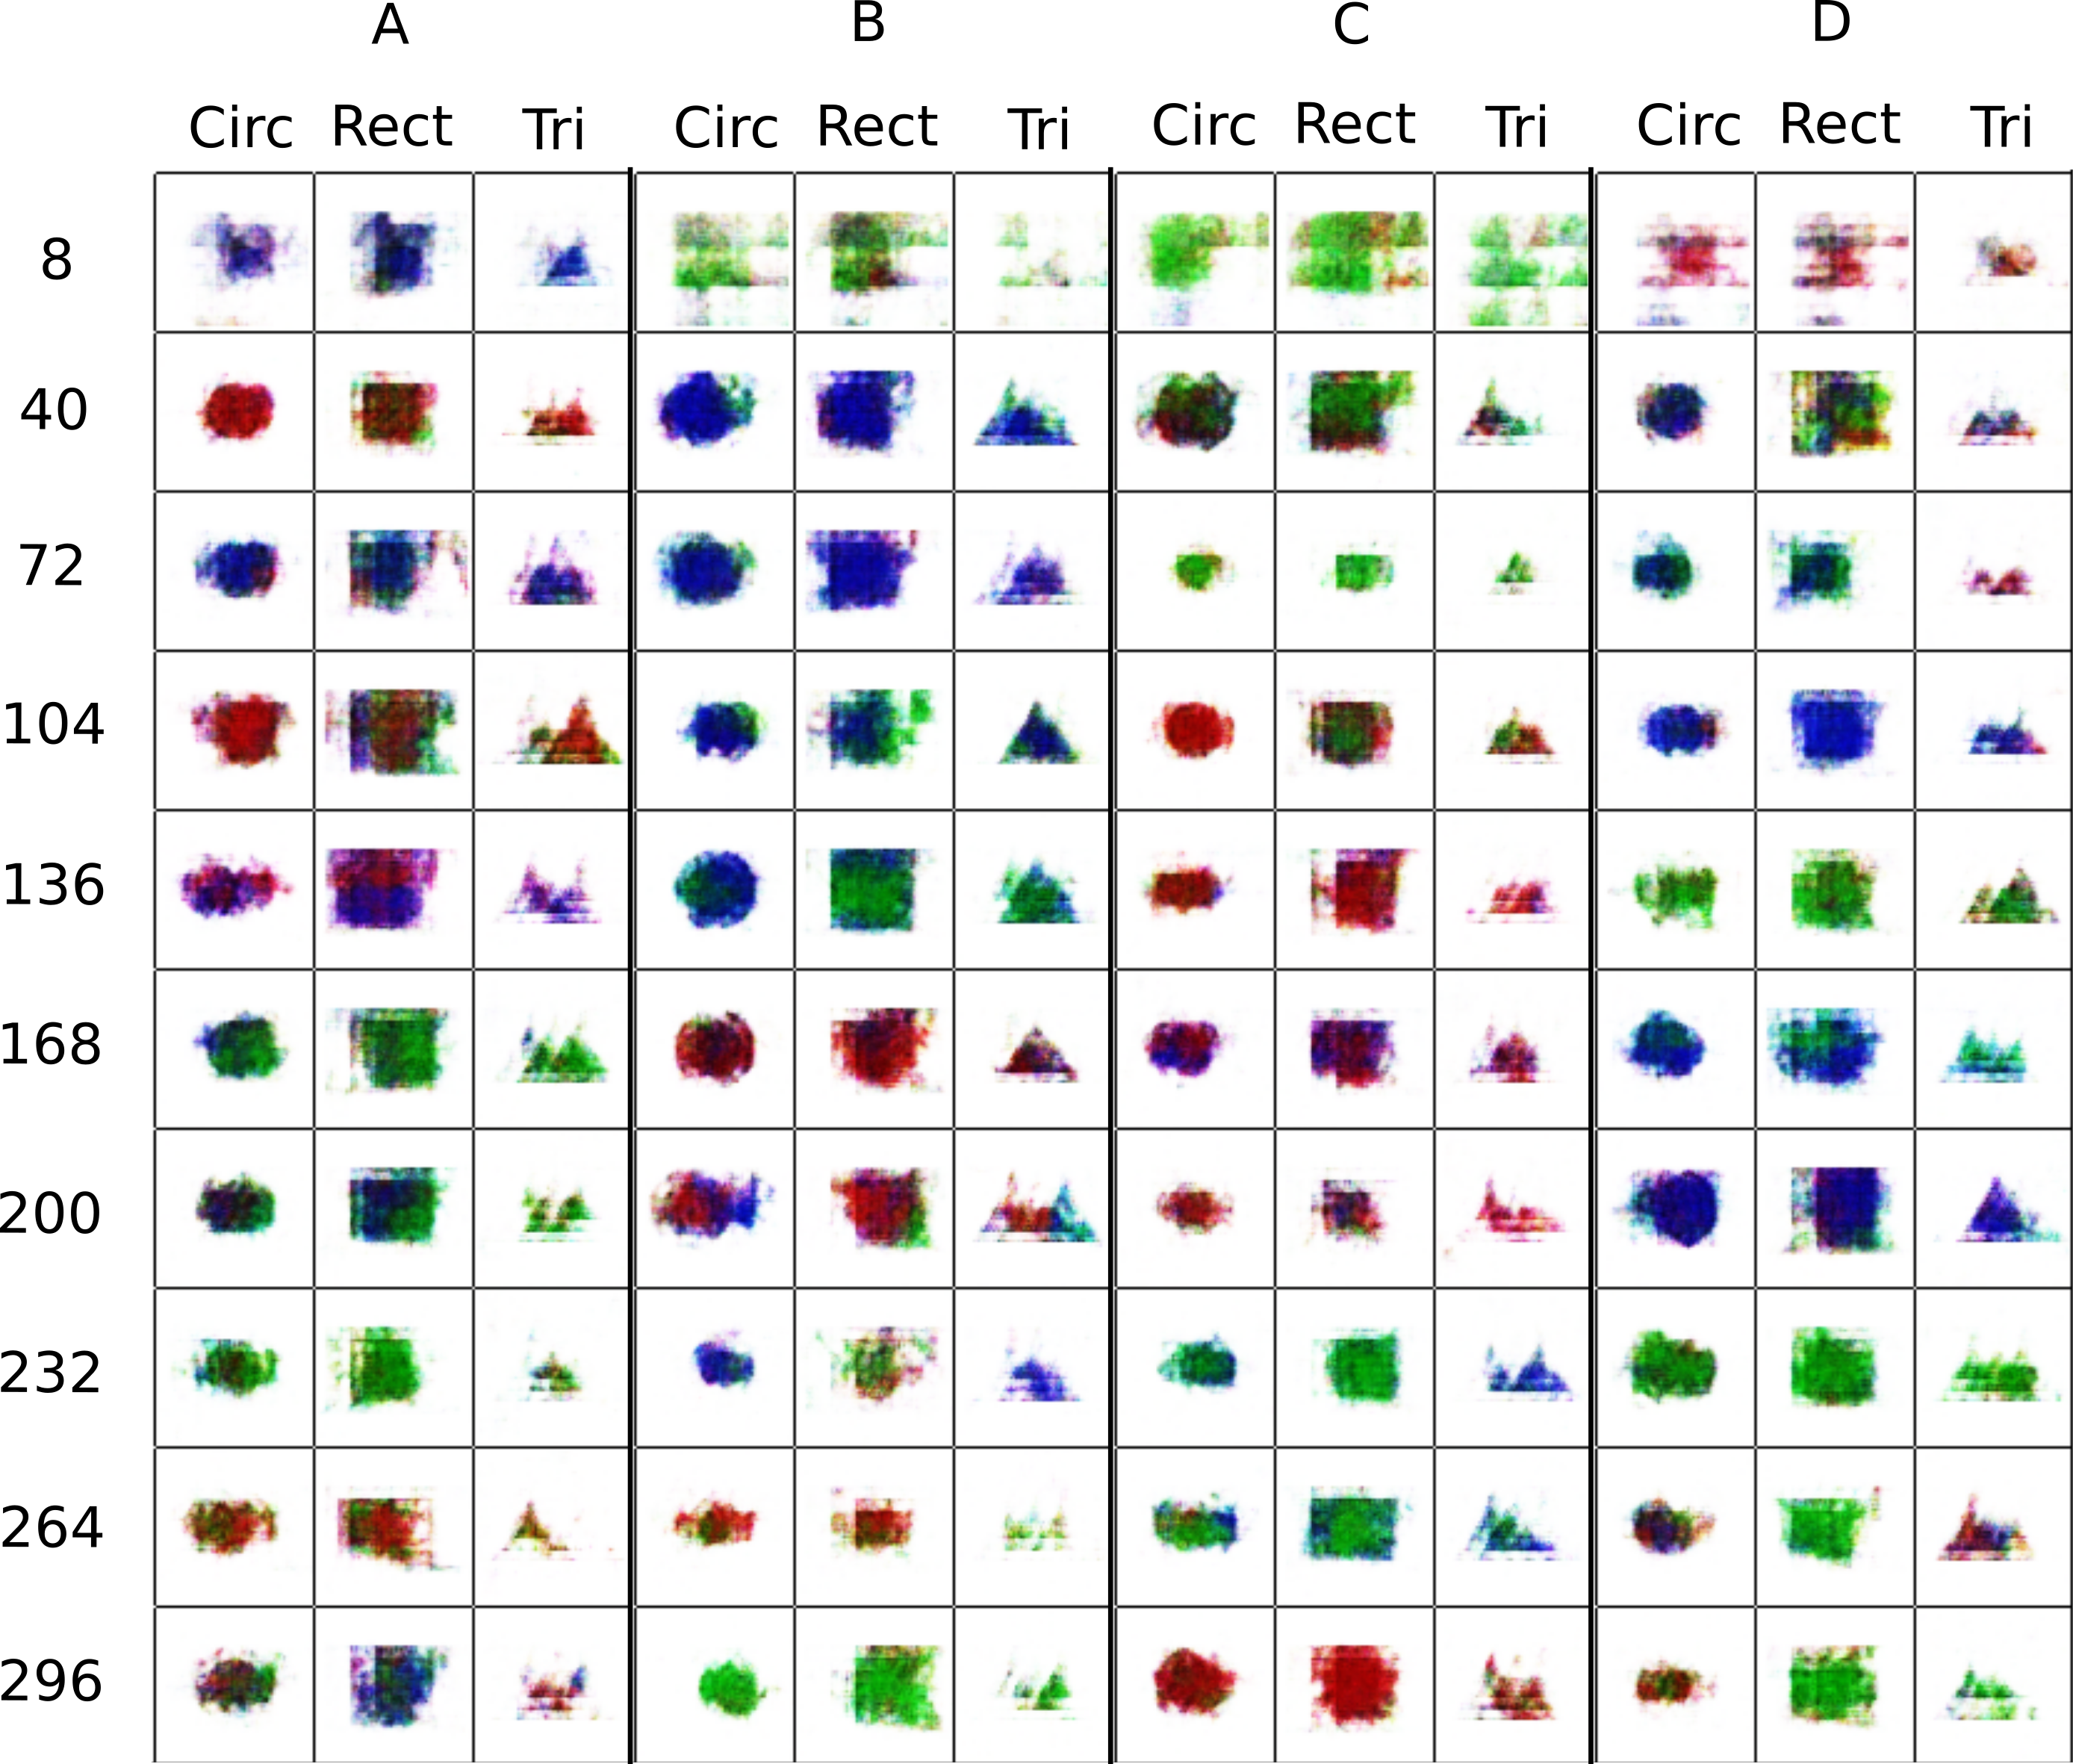
\includegraphics[width=0.75\textwidth]{Figs/shapes/shapes333.png}
\caption{Experiment 2, runs A-D:  Images generated of each shape for different emedding sizes.}
\label{fig:shapes333}
\end{figure}

Whilst an embedding size of 136 neurons disentangled the meanings of \textsc{Circle}, \textsc{Rectangle} and \textsc{Triangle} in run B of experiment 2, this result was not consistent across all four runs (or for any other embedding size) as seen in \autoref{fig:shapes333}. This indicates that the weight initialisation and data selection have an effect on whether the \ac{MAE} can learn the meanings of the shape names (\textsc{Circle}, \textsc{Rectangle} and \textsc{Triangle}) when additional object sizes are added to the training data.


\begin{figure}[h]
\centering
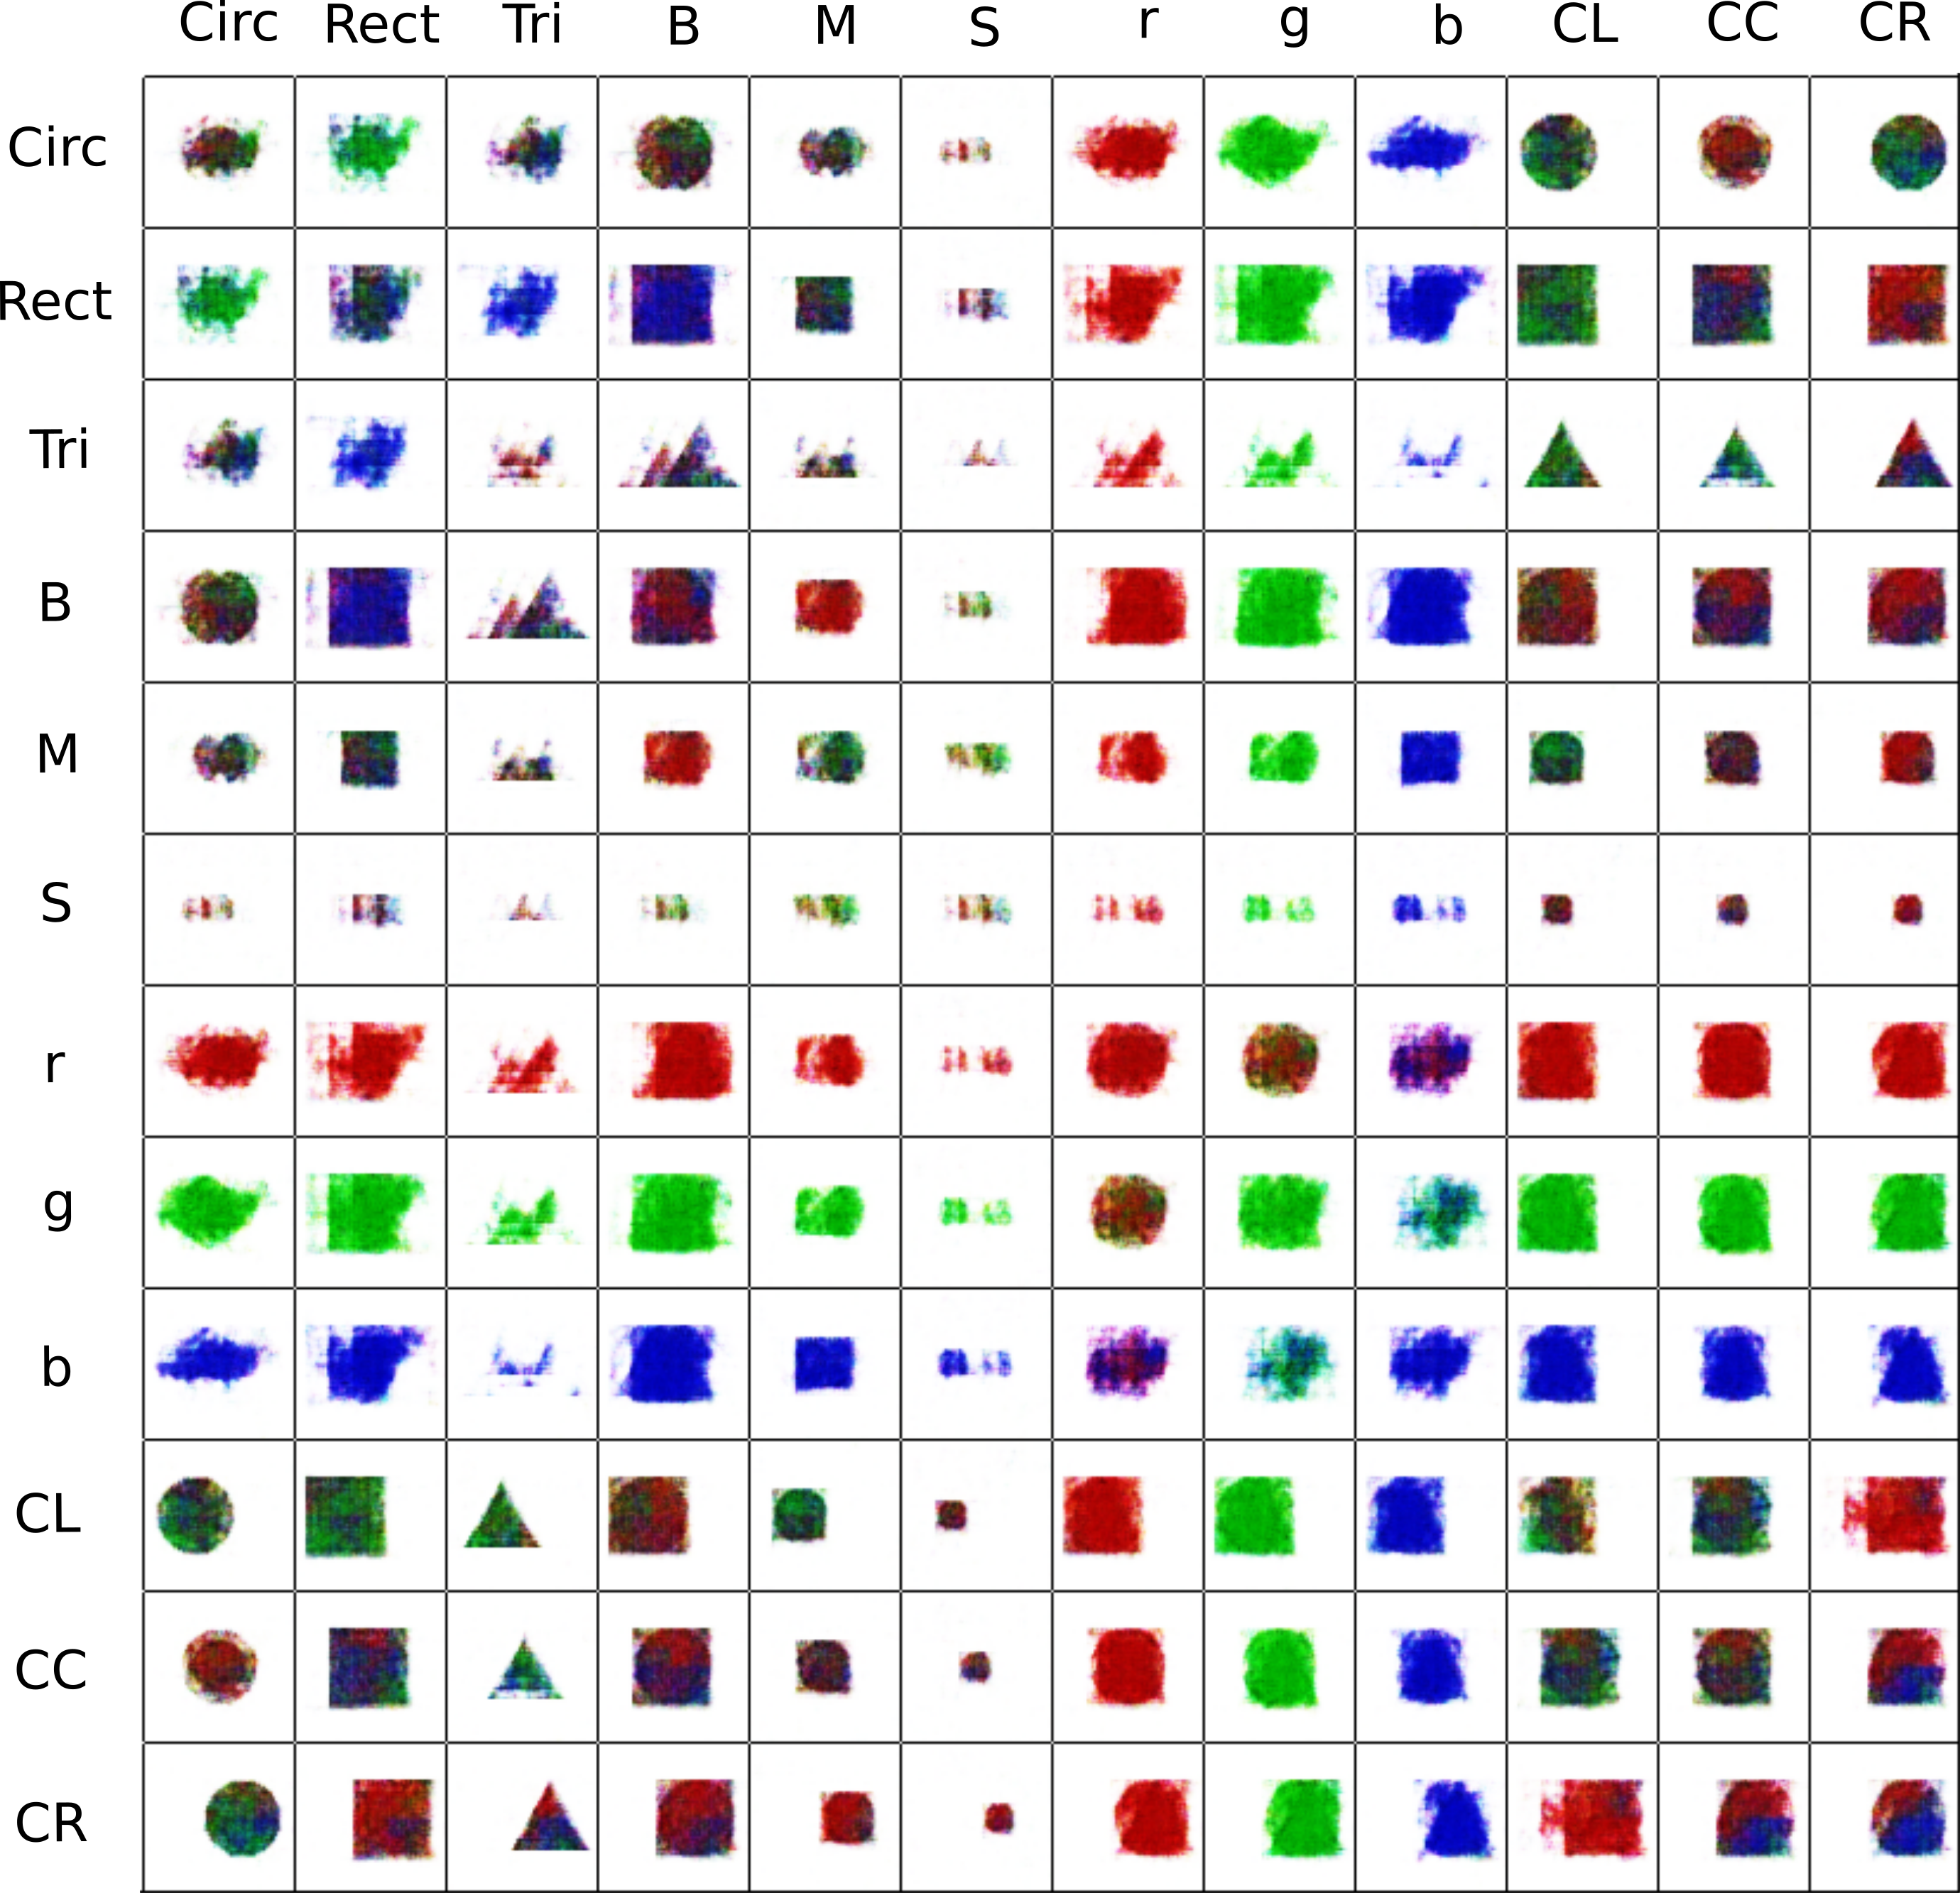
\includegraphics[width=0.75\textwidth]{Figs/shapes/2word333A.png}
\caption{Experiment 2, run A:  Images generated using word pairs using an embedding size of 296 neurons.}
\label{fig:2word333}
\end{figure}

Another way to inspect the quality of the learnt embedding is to provide pairs of words to the \ac{MAE} and observe what it generates as output. \autoref{fig:2word333} shows the output of the \ac{MAE} trained in run A of experiment 2 (runs B-D can be found in the supplimental material) with an embedding size of 296 neurons. Here the \ac{MAE} is correctly generating images from the words \textsc{Circle}, \textsc{Rectangle} and \textsc{Triangle} as well as the other words in its ``vocabulary''. The diagonal of \autoref{fig:2word333} is the equivalent of the bottom row (296) of \autoref{fig:333single}. The addition of a second word allows for the correct generation of the three shapes in different positions and sizes, suggesting that when only the shape is provided as input, the \ac{MAE} does not know where to draw the object or how big to draw it. By adding a second word and removing some uncertainty, the output of the \ac{MAE} is much more well defined. This is a particularly strong result in the case of when a position is provided in conjuction with either a shape, size or colour. 


\paragraph{Description Accuracy}
Even with the added complexity of the additional sizes, the MAE gets 100\% accuracy in all testing conditions for all embedding sizes. 


\subsubsection{Discussion}

Increasing the number of variable attributes in the dataset, i.e. adding the extra sizes, has had a negative affect on the ability of the \ac{MAE} to ground the meanings of each of the words in the descriptions. This is highlighted when the results of experiments 1 and 2 are seen side by side as in \autoref{fig:shapes333v331}. 

\begin{figure}[h]
\centering
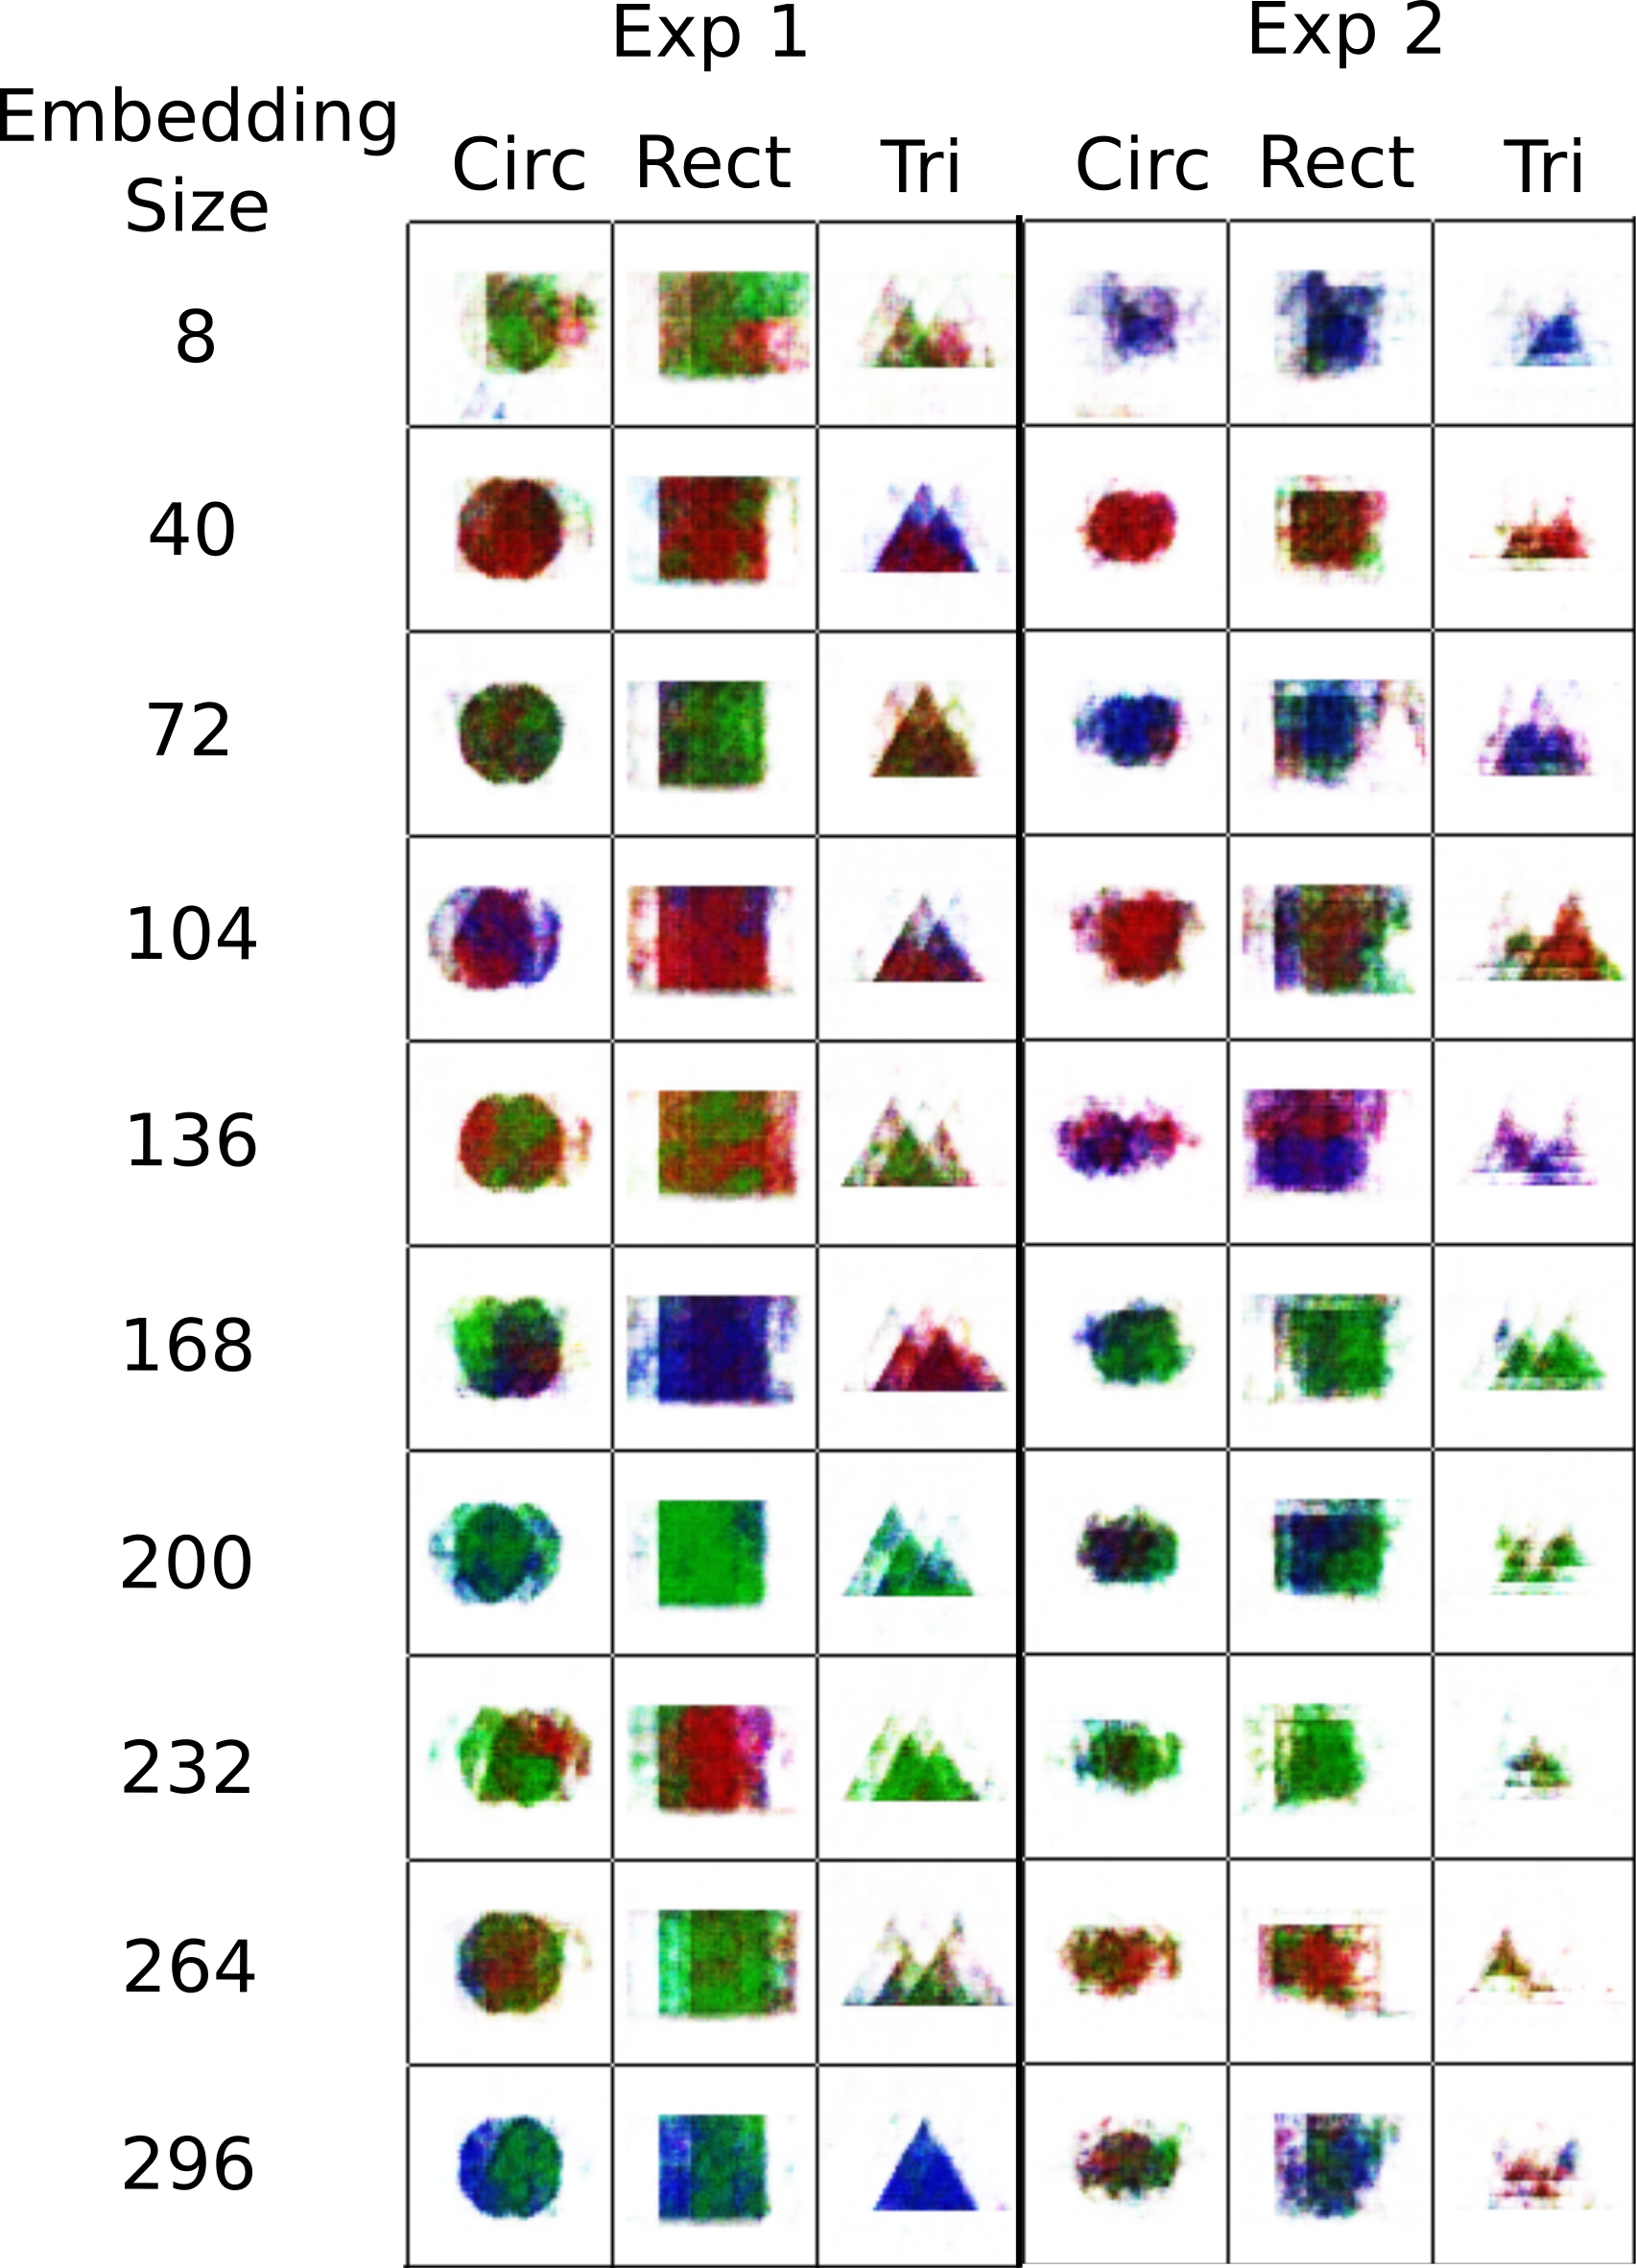
\includegraphics[width=0.5\textwidth]{Figs/shapes/shapes331v333.png}
\caption{Images generated of each shape for different sizes of embedding using the \acp{MAE} trained in experiments 1 and 2 run A.}
\label{fig:shapes333v331}
\end{figure} %This issue could likely be solved by the addition of more examples per object.
However, the \ac{MAE} remains able to accurately generate images from full descriptions (see \autoref{fig:333multi}). 
An embedding size of 296 neurons gave the all around best performance in experiment 2 and performed the best at symbol grounding in experiment 1, therefore it will be used for the later experiments.

This experiment demonstrates that Hypothesis 3: \ac{MRL} can be used to learn language as it relates to the visual properties of objects, continues to hold true even for more complex data. As Ngiam et al. were able to demonstrate that \acp{MAE} are able to learn the association between video and phonemes, which is much more complex data than that used here as both have a time dependancy, it is unsurprising that the \ac{MAE} has been able to achieve symbol grounding for this datasubset.

\newpage
\subsection{Experiment 3}


\begin{table}[h]
\centering
\begin{tabular}{|c|c|}
\hline
\textbf{Attribute} & \textbf{Description} \\ \hline \hline
\textbf{Shapes} & \textbf{Corners} \\ \hline
Rectangle & 4\\ \hline
Triangle & 3\\ \hline
Circle & 0\\ \hline 

\textbf{Colours} & \textbf{RGB Values}	\\ \hline	
Red & (75,0,0) - (255, 10, 10)\\ \hline
Green  & (0,75,0) - (10, 255, 10)\\ \hline
Blue   & (0,0,75) - (10, 10, 255)\\ \hline

\textbf{Sizes} & 	\textbf{Length/Radius (pixels)} \\ \hline			  
Big    & 32 - 35  \\ \hline
Medium & 22 - 25 \\ \hline
Small  & 12 - 15 \\ \hline 

\textbf{Positions} & \textbf{Object Centre Coordinate}	\\ \hline					  
Top Left & (22,42)\\ \hline	
Top Centre & (32,42)\\ \hline
Top Right & (42,42)\\ \hline
Centre Left &(22,32)\\ \hline
Centre & (32,32)\\ \hline
Centre Right &(42,32)\\ \hline
Bottom Left & (22,22)\\ \hline
Bottom Centre & (22,42)\\ \hline
Bottom Right & (42,22)\\ \hline				
\end{tabular}
\caption{Experiment 3 data-subset.}
\label{tab:exp3_data} 
\end{table}

This experiment adds further vairety to the data, adding an additional 6 positions as seen in \autoref{tab:exp3_data}. In this experiment, I also observe how incrementally learning these new properties affects the quality of the generated outputs as well as the bidirectional grounding of the different words from the descriptions and visual attributes of the images. 

As was explained in \autoref{Chapter3}, humans do not learn everything from scratch, instead we bootstrap new skills on top of previosuly learnt ones. In fact, even new born babies do not start learning from scratch as was seen in \cite{webb2015mother, fantz1963pattern, reid2017human}, developmental learning starts prenatally and continues throughout our lives. As such, this experiment aims to test hypothesis 4: \ac{MRL} can be improved through transfer learning, and demonstrates how a develpmental approach to training neural networks can improve their learning.

Incremental learning is performed by transfering the weights learned in the previous experiments and then performing further training on the data-subset of experiment 3. This is similar to the approach taken in \cite{vinyals2015show, venugopalan2014translating, johnson2016densecap} where pretraining on image classification and language prediction tasks was used to initialise image captioning systems. This approach was not necessary in experiment 2 as the \ac{MAE} was able to achieve 100\% description accuracy when trained from scratch. By comparing the quality of the output from a \ac{MAE} trained starting from random weights, with the \ac{MAE} pretrained in experiments 1 and 2 (after they train on the data for experiment 3), I will answer the fundamental question of whether, having knowledge of the meaning of a subset of words and visual attributes, aids the learning of new words and image attributes.

To make this a fair comparison, the MAE which is initialised with random weights will be trained for 100 epochs so that the total number of epochs of training that each \ac{MAE} receives is equal. I.e. either 50 epochs pretraining and 50 epochs training or 100 epochs of training.

Unlike in the previous two experiments, the embedding size will be fixed to 296 neurons as this gave the best performance in experiment 2.

The different initialisation schemes will be referred to as: Random: randomly initialised weights, Exp1: initialisation with the weights trained during experiment 1 and Exp2: initialisation with the weights trained during experiment 2.

\subsubsection{Results}
Using random initialisation as a starting point for experiment 3 leads to the lowest reconstruction error as seen in \autoref{tab:res339}. The lower reconstruction error during testing does not translate to improved symbol grounding.


\begin{table}[h!]
\centering
	\begin{tabular}{|c|c|c|c|}
	\hline
	\textbf{Initialisation} & 	\textbf{Bimodal} & \textbf{Image Only} 	& 	\textbf{Words Only} \\ \hline
	Random	&	\textbf{3.97}	$\mypm$	0.41	&	22.73	$\mypm$	35.14	&	\textbf{4.09}	$\mypm$	0.27\\ \hline
	Exp 1 	&	5.29	$\mypm$	0.47	&	6.69	$\mypm$	3.48	&	5.78	$\mypm$	0.33	\\ \hline
	Exp 2 	&	5.33	$\mypm$	0.31	&	\textbf{5.06}	$\mypm$	0.38	&	5.75	$\mypm$	0.24	\\ \hline

	\end{tabular}
\caption{Experiment 3: Total MSE for different weight initialisations. (All values are $\times10^{-3}$.)}
\label{tab:res339}
\end{table}


\paragraph{Image Generation}
It is not feasable to show every combination of shape, colour, size and position, so in \autoref{fig:339multi} a selection of these combinations are shown.

\begin{figure}[h]
\centering
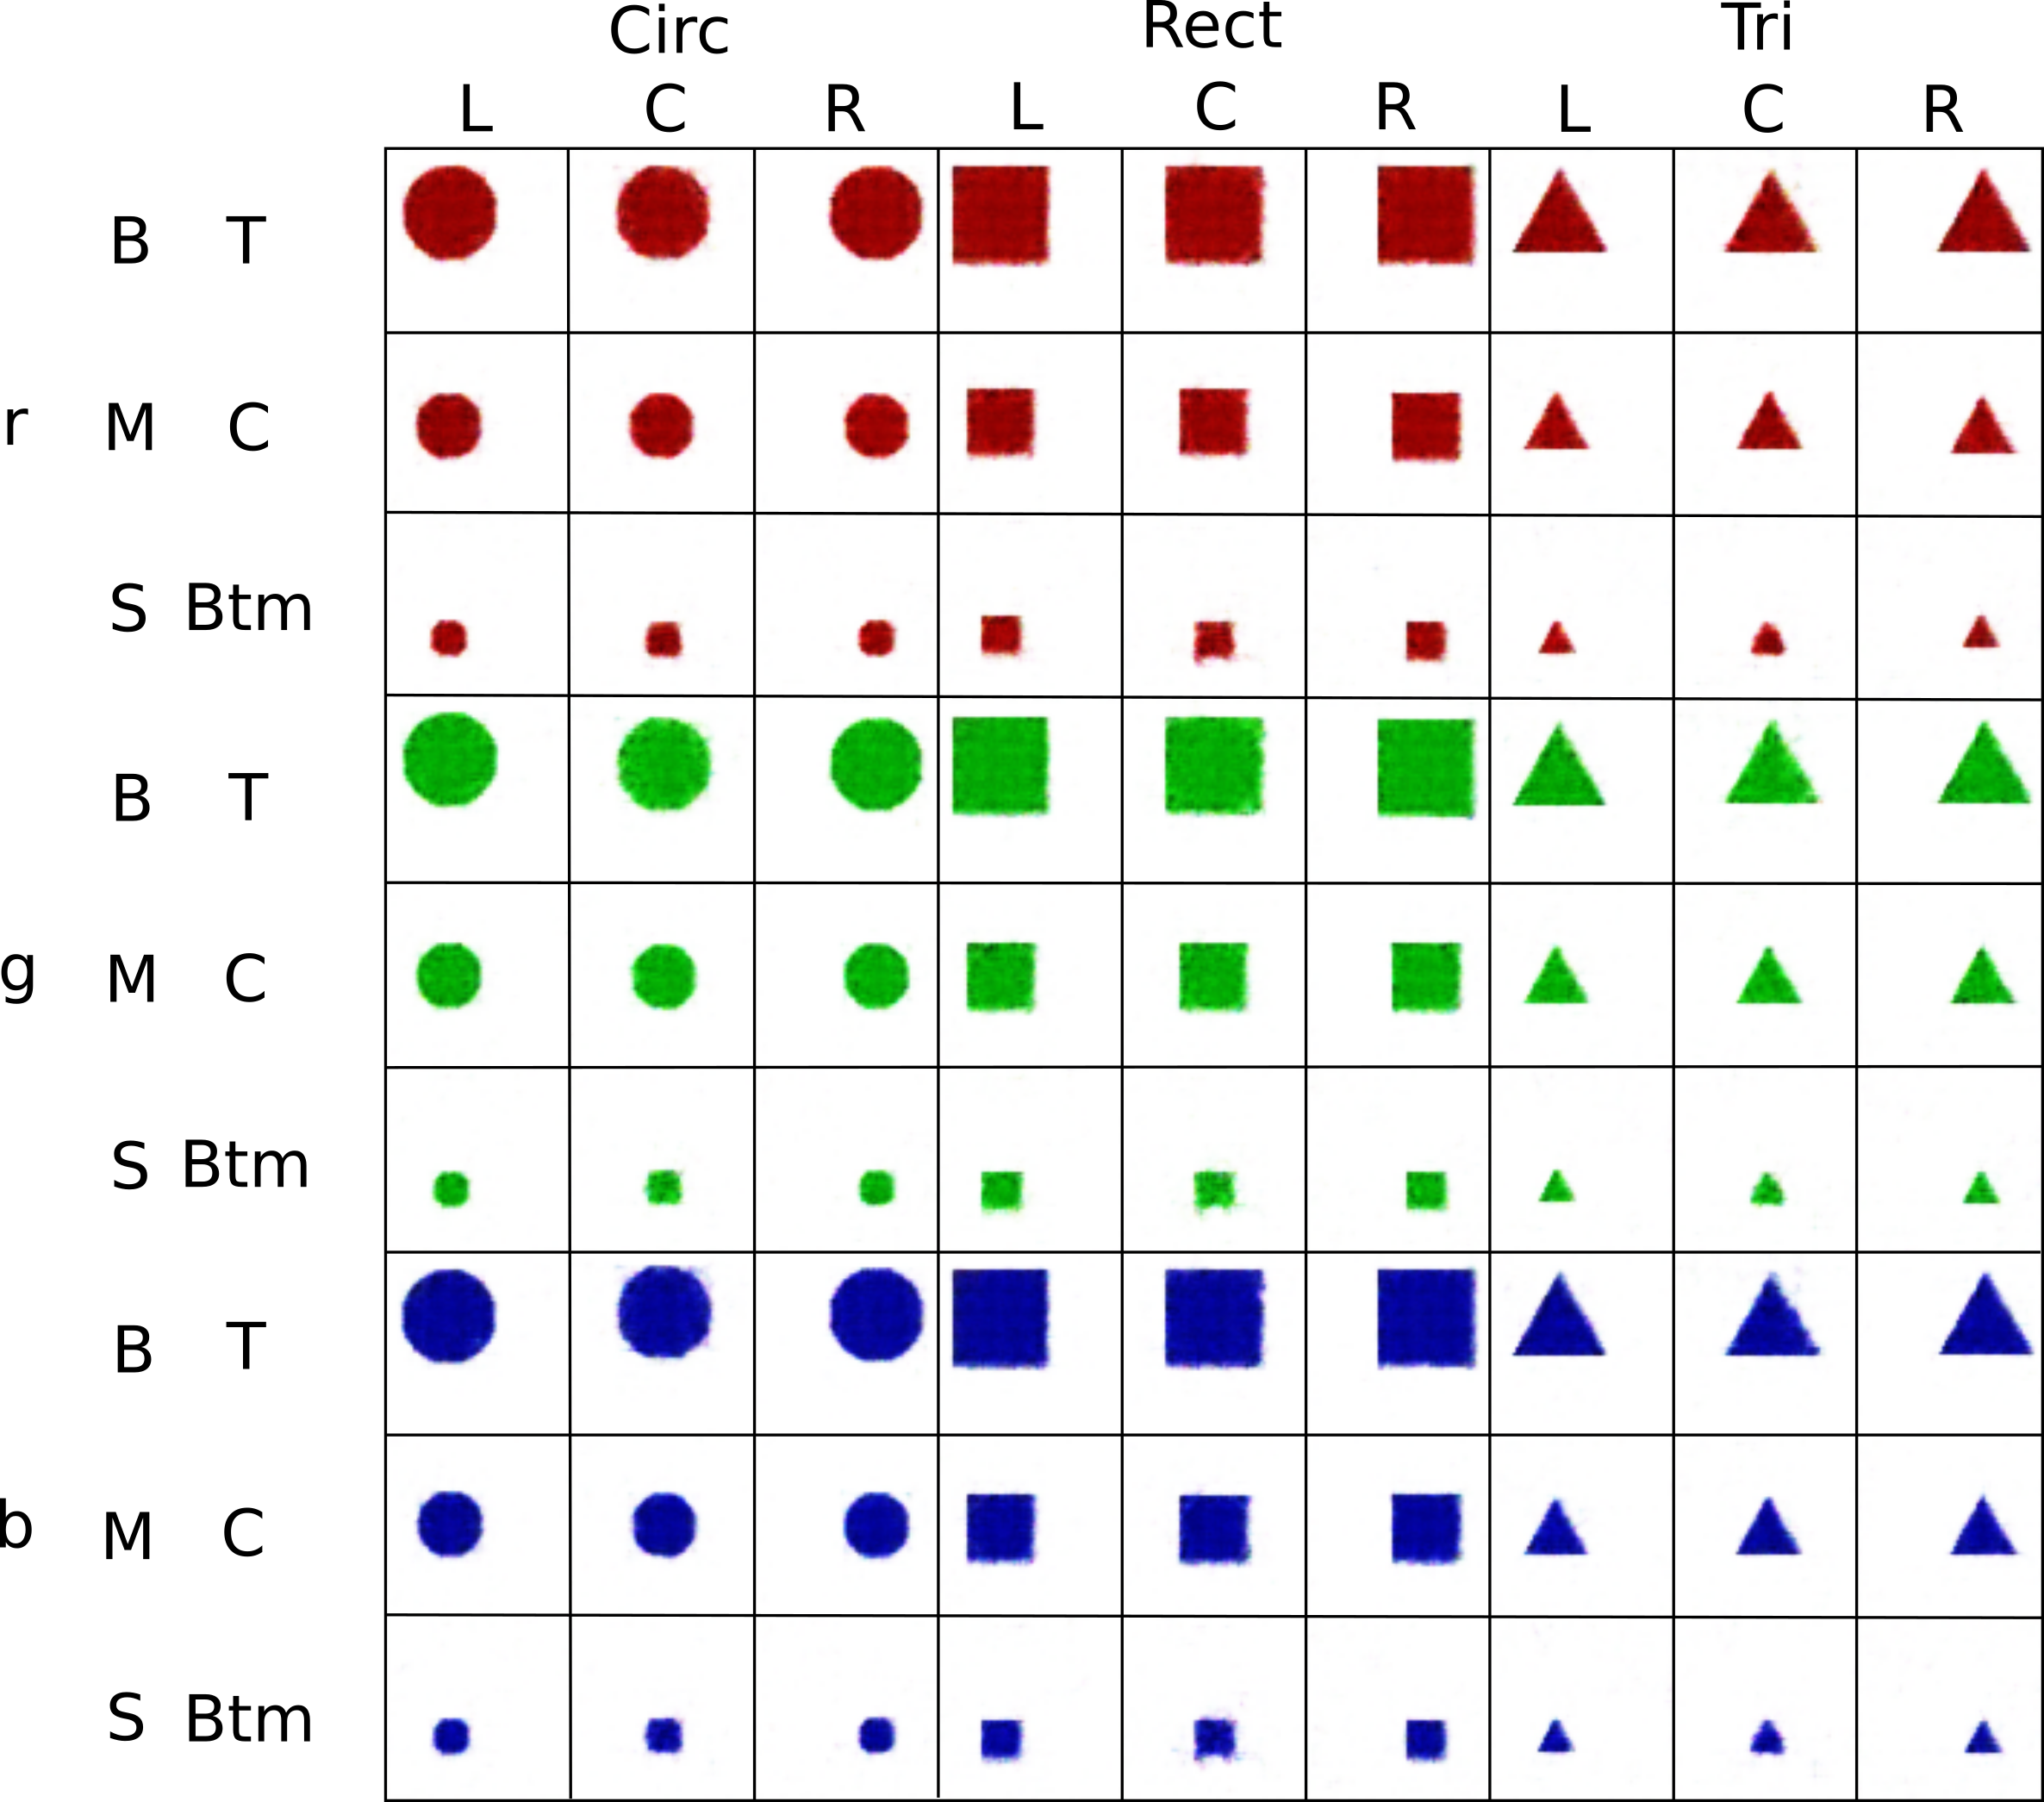
\includegraphics[width=0.625\textwidth]{Figs/shapes/multiword339.png}
\caption{Experiment 3, run A: Images generated from descriptions, starting training from randomly initialised weights.}
\label{fig:339multi}
\end{figure}

The addition of new positions has had an effect on the quality of the images generated from descriptions by the \ac{MAE}. The images have become blurrier compared to images generated in previous experiments. However they are still easily recognisable as matching their descriptions.

When only given a single word as input, as in \autoref{fig:339single}, the MAE is not able to correctly generate any of the shapes (\textit{Circle}, \textit{Rectangle}, \textit{Triangle}). Unlike in experiment 2, where the words \textsc{Circle}, \textsc{Rectangle} and \textsc{Triangle} lead to the generation of visual attributes which match these words, in experiment 3 it is unclear that these visual attributes can be seen.

The colours are all correctly generated and again, the sizes show a clear relation with the most pixels being coloured for \textsc{big} matching the visual attribute \textit{Big} and the least for \textsc{small} matching the visual attribute \textit{Small}.

\begin{figure}[h]
\centering
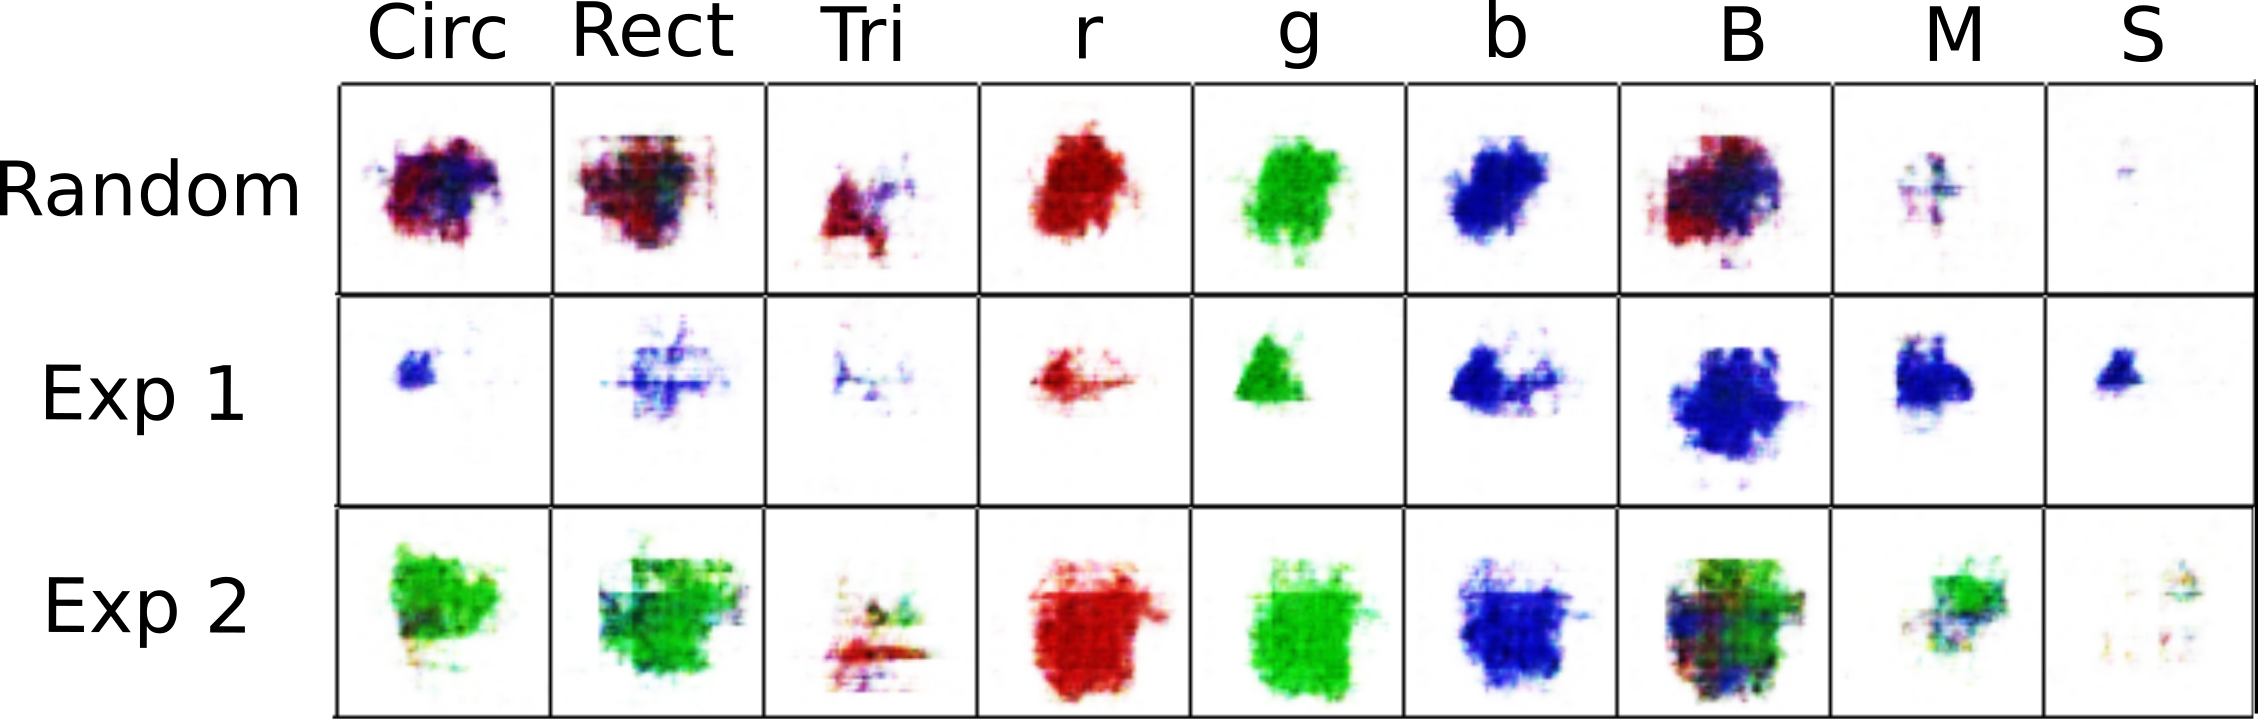
\includegraphics[width=0.75\textwidth]{Figs/shapes/singlelabel339.png}
\caption{Experiment 3, run A: Images generated from shape, colour and size words for different weight initialisation conditions.}
\label{fig:339single}
\end{figure}

The new positions are correctly learnt with a clear distinction between positions on the top, centre and bottom as well as left, centre and right and their combinations (e.g. bottom right) as seen in \autoref{fig:339single_pos}.

\begin{figure}[h]
\centering
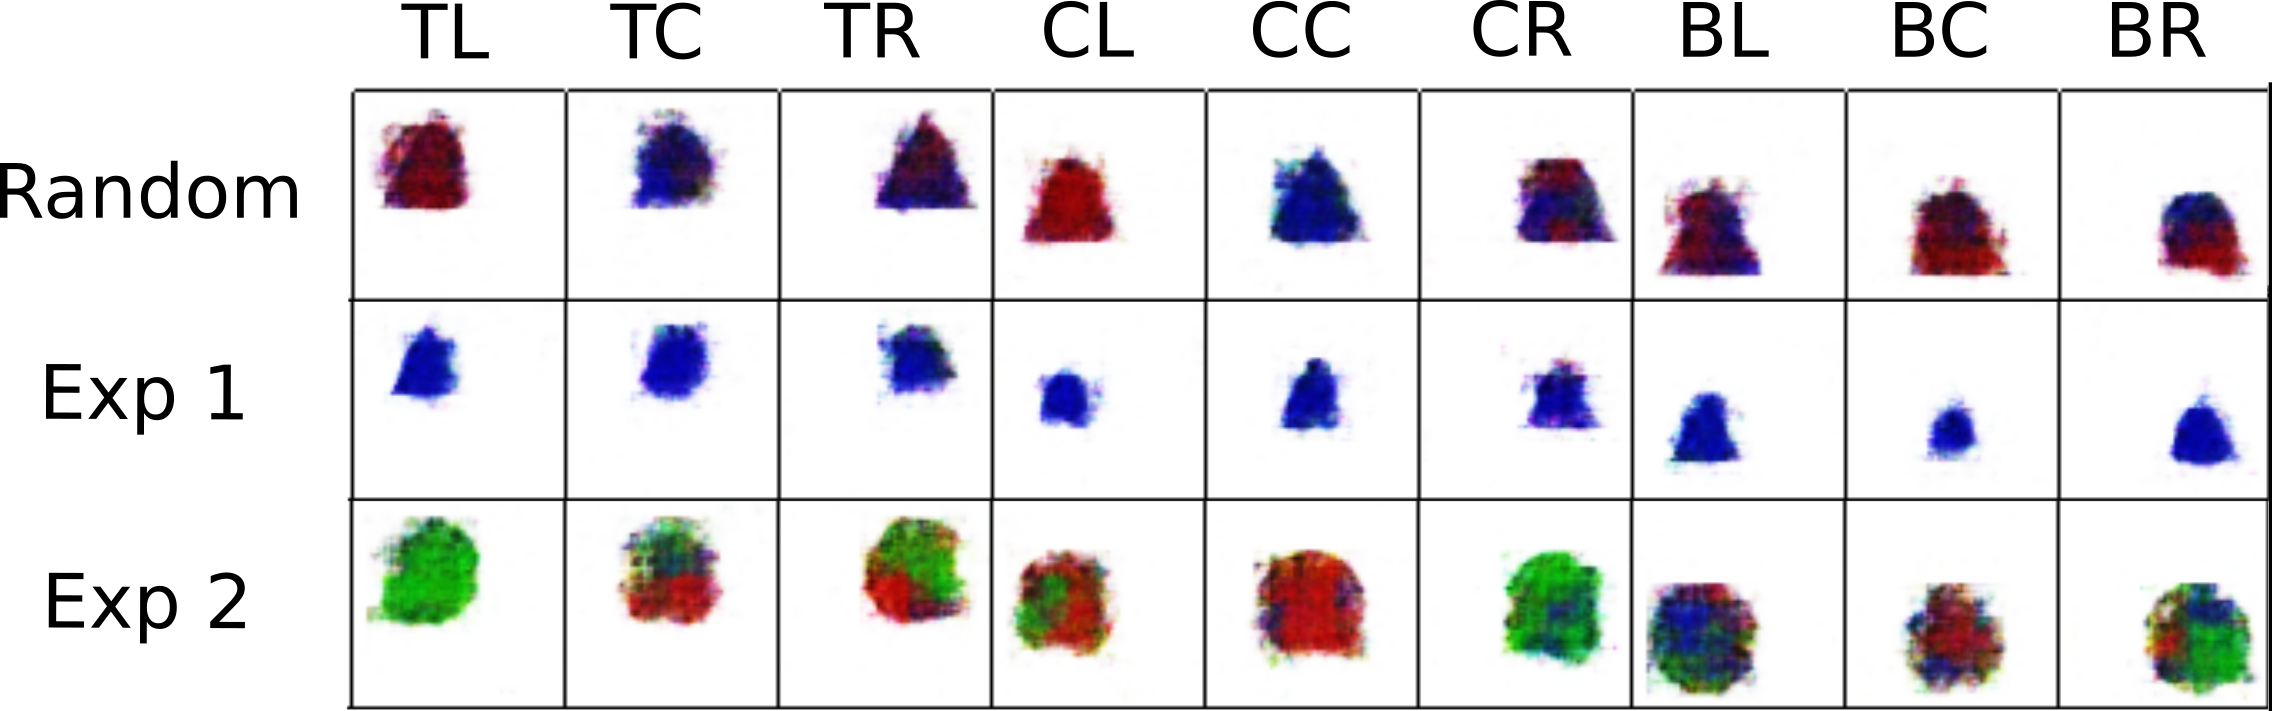
\includegraphics[width=0.75\textwidth]{Figs/shapes/singlelabel339_pos.png}
\caption{Experiment 3, run A: Images generated from each position word for different weight initialisation conditions.}
\label{fig:339single_pos}
\end{figure}


As in experiment 2, the addition of a second word as input, leads to better reconstruction of the visual attributes with which they are associated. \autoref{fig:2word339} shows a comparison of the three different weight initialisations after training. It is clear in all three cases that the \ac{MAE} learns to correctly ground the words \textsc{Circle}, \textsc{Rectangle} and \textsc{Triangle}. However, in the case of initialising with weights from experiment 1, the pretraining results in a worse performance than random weights.
\begin{figure}[h]
\centering
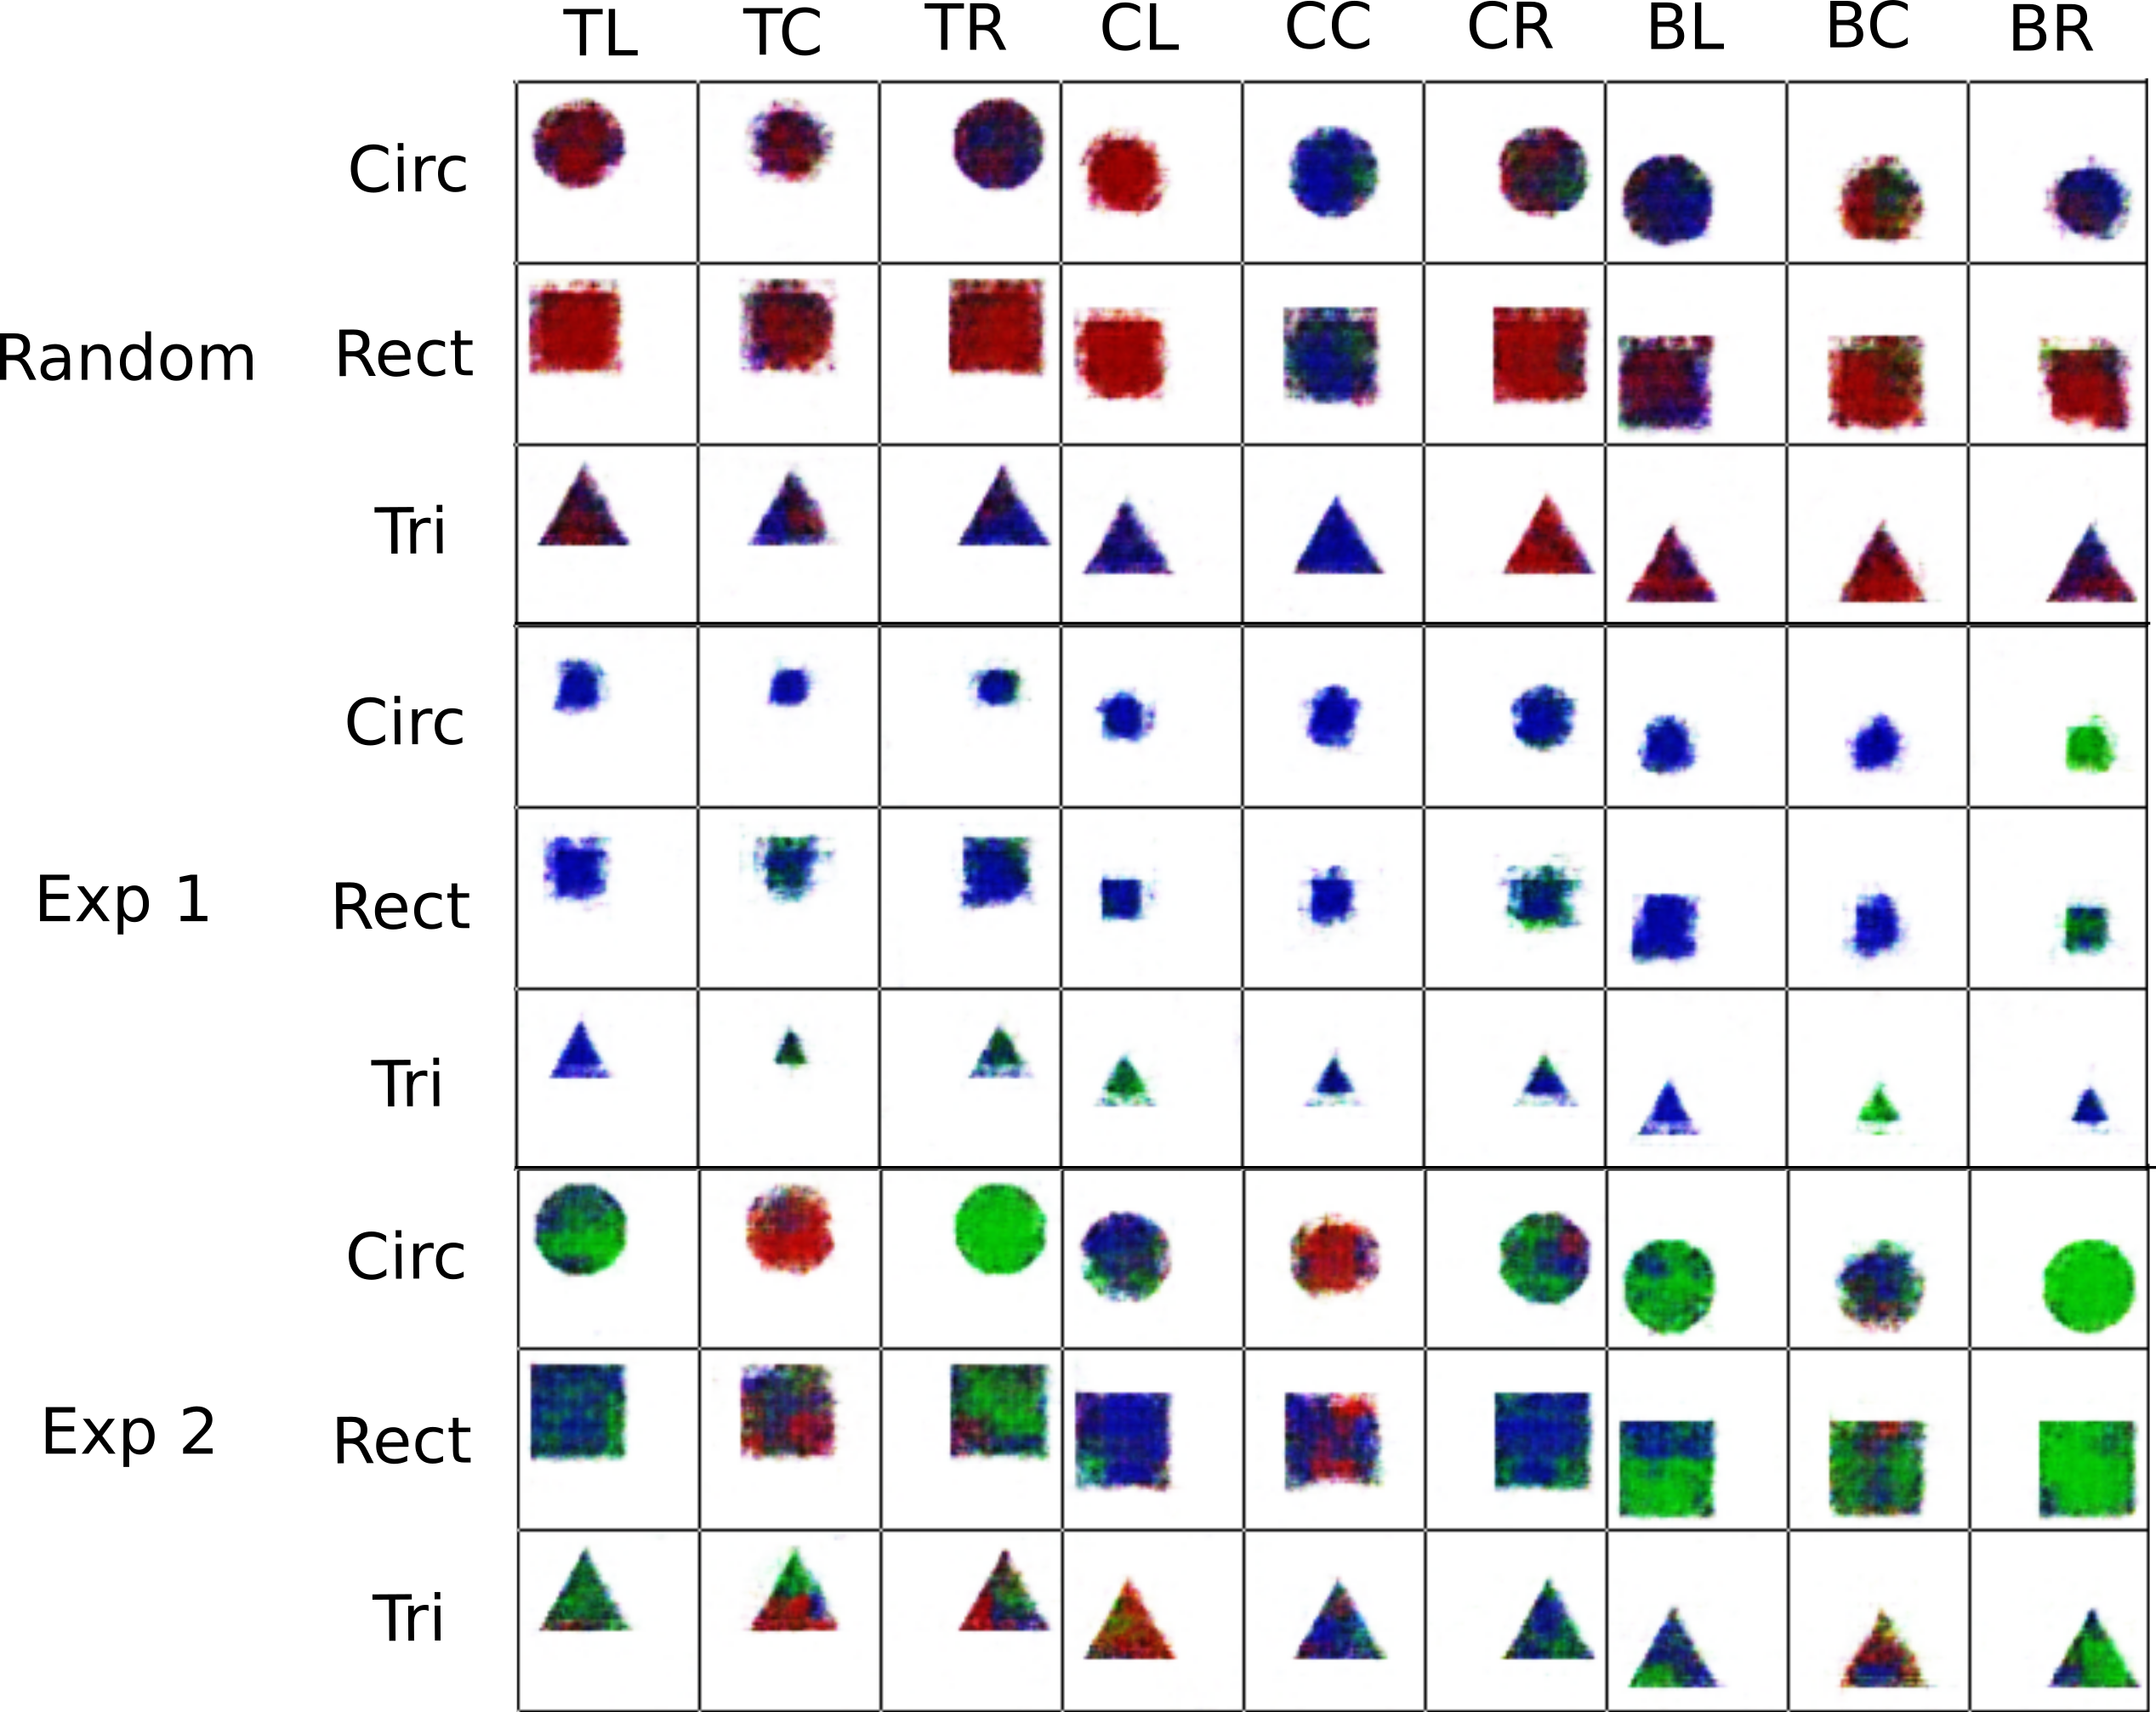
\includegraphics[width=0.75\textwidth]{Figs/shapes/2word339_pos.png}
\caption{Experiment 3, run A: Images generated using word pairs.}
\label{fig:2word339}
\end{figure}

Initialising with weights from experiment 2 offers a marginal benefit, with each of the shapes being more solid in appearance. Full results from all four runs can be found in the supplimental materials.

\paragraph{Description Accuracy}

\begin{table}[h!]
\centering
	\begin{tabular}{|c|c|c|c|}
	\hline
	\textbf{Initialisation} & 	\textbf{Bimodal} & 	\textbf{Image Only} 	& 	\textbf{Words Only} \\ \hline
	Random	&	100.00	$\mypm$	0.00	&	98.51	$\mypm$	4.52	&	100.00	$\mypm$	0.00	\\ \hline
	Exp 1	&	100.00	$\mypm$	0.00	&	99.85	$\mypm$	0.50	&	100.00	$\mypm$	0.00	\\ \hline
	Exp 2	&	100.00	$\mypm$	0.00	&	\textbf{99.99}	$\mypm$ 0.03	&	100.00	$\mypm$	0.00	\\ \hline



	\end{tabular}
\caption{Experiment 3: Percentage Description Accuracy for different weight initialisations. }
\label{tab:res339_acc}
\end{table}

There is a clear effect on the accuracy of descriptions generated by the \ac{MAE} when transfer learning is used. This is seen as the improved performance when generating descriptions in the Image Only testing condition as seen in \autoref{tab:res339_acc} where the \ac{MAE} pretrained on experiment 2 only incorrectly described 1 image compared to the \ac{MAE} trained from scratch which incorrectly described 181 images.


\subsubsection{Discussion}
Though the addition of extra positions had a detrimental effect on the generation of images from single words, (see \autoref{fig:339single} and \autoref{fig:339single_pos}) the \ac{MAE} was still able to correctly learn to ground all of the words of the descriptions. This becomes apparent when pairs of words are provided as input, as in \autoref{fig:2word339}.

Taking an incremental approach to training by pretraining on a simpler task does not have a universally positive effect on the grounding of words to visual attributes. Whilst the weights from experiment 2 provided a small but noticable benefit when generating images from pairs of words over the random initialisation baseline, the weights from experiment 1 did not. 

\begin{table}
\centering
\begin{tabular}{|c|c|}
\hline
\textbf{Initialisation} & \textbf{Total Weight Updates}\\ \hline
Random &  1,215,000\\ \hline
Exp 1 &  540,000\\ \hline
Exp 2 &  810,000\\ \hline

\end{tabular}
\caption{Experiment 3: Total number of weight updates.}
\label{tab:updatesTotal}
\end{table}

Despite the \ac{MAE} initialised with Random weights receiveing more total updates to its weights as seen in \autoref{tab:updatesTotal}, its performance is worse than both the \ac{MAE} pretrained on experiment 1 and the MAE pretrained on experiment 2 in terms of both error and accuarcy in the Image only Testing Condition. See \autoref{appendix:app5} for an explanation of how the number of weight updates is calculated.

Having the \ac{MAE} master the simpler tasks of either experiment 1 or 2 through pretraining, had a positive effect on both image and description generation in the Image Only testing condition. This also carried over to the accuracy of description generation in this condition. This shows that by first learning to ground a smaller number of visual attributes to the words that describe them, the \ac{MAE} is better able to correctly learn the additional words of the new data-subset (improved description accuracy) and be more confident about the meaning of these visual attributes (lower \ac{MSE}).


\newpage
\subsection{Experiment 4}
For this experiment I will make use of all of the data in ArtS as shown in \autoref{tab:Arts_desc}. Again, I explore the affects of incremental learning, utilising the prelearned weights of experiments 1 and 2 and 3. This will allow me to examine whether having a larger number of concepts (words and their image equivalents) mastered  helps learning new concepts or whether one can simply learn all concepts simultaneously. In humans, we have the advantage of being able to build off of previously learnt skills when approaching new tasks. In \cite{webb2015mother, fantz1963pattern, reid2017human}, it is shown that babies start to develop their visual and auditory abilities even before birth. They then build off of these basic skills to learn more complex abilities like speaking, understanding speech and eventually, even more complex skills such as mathematics, painting or playing a musical instrument, to name but a few.

The different initialisation schemes will be referred to as: Random: randomly initialised weights, Exp1: the weights trained during experiment 1, Exp2: the weights trained during experiment 2, Exp 3: the weights trained during experiment 3 starting from random initialisation.
%, Exp 1+3: the weights trained during experiment 3 starting with the weights from experiment 1, Exp 2+3: the weights trained during experiment 3 starting with the weights from experiment 2.
%Two other conditions, Random 80 and Random 100 utilise a random initialisations but have 80 and 100 samples per object respectively compared to the 50 samples per object used in all other conditions.
%

\subsubsection{Results}

\begin{table}[h!]
\centering
	\begin{tabular}{|c|c|c|c|}
	\hline
	\textbf{Initialisation} & 	\textbf{Bimodal} & 	\textbf{Image Only} 	& 	\textbf{Words Only} \\ \hline
Random 	&	3.82	$\mypm$	0.30	&	54.12	$\mypm$	43.74	&	3.96	$\mypm$	0.22	\\ \hline
Exp 1	&	\textbf{3.73}	$\mypm$	0.06	&	9.33	$\mypm$	9.71	&	\textbf{3.91}	$\mypm$	0.04\\ \hline
Exp 2	&	3.80	$\mypm$	0.19	&	\textbf{8.55}	$\mypm$	4.70	&	3.96	$\mypm$	0.20	\\ \hline
Exp 3	&	3.75	$\mypm$	0.02	&	14.28	$\mypm$	12.18	&	3.93	$\mypm$	0.05	\\ \hline
%Exp1+3	&	3.77	$\mypm$	0.14	&	16.17	$\mypm$	17.96	&	3.97	$\mypm$	0.13	\\ \hline
%Exp 2+3	&	3.76	$\mypm$	0.12	&	33.08	$\mypm$	57.02	&	3.92	$\mypm$	0.06	\\ \hline

	\end{tabular}
\caption{Experiment 4: Total MSE for different weight initialisations. (All values are $\times10^{-3}$.)}
\label{tab:res739}
\end{table}

The results for each method of initialising the weights of the \ac{MAE} in experiment 4 can be seen in \autoref{tab:res739}. Whilst in the Bimodal and Words Only testing conditions, initialising with random weights generated a comparable loss, this is not the case in the Image Only testing condition where the random weight initialisation performs an order of magnitude worse than any of the other initialisation schemes.


\paragraph{Image Generation}

Once again there is a distinction between the three sizes as shown in \autoref{fig:739single_shape}, this is independent of initialisation condition. However, whilst there are clear distinctions between the three shapes for all initialisation conditions, with the exception of initialising with weights from experiment 2 it is not clear that the shapes have been correctly learnt.

\begin{figure}[h]
\centering
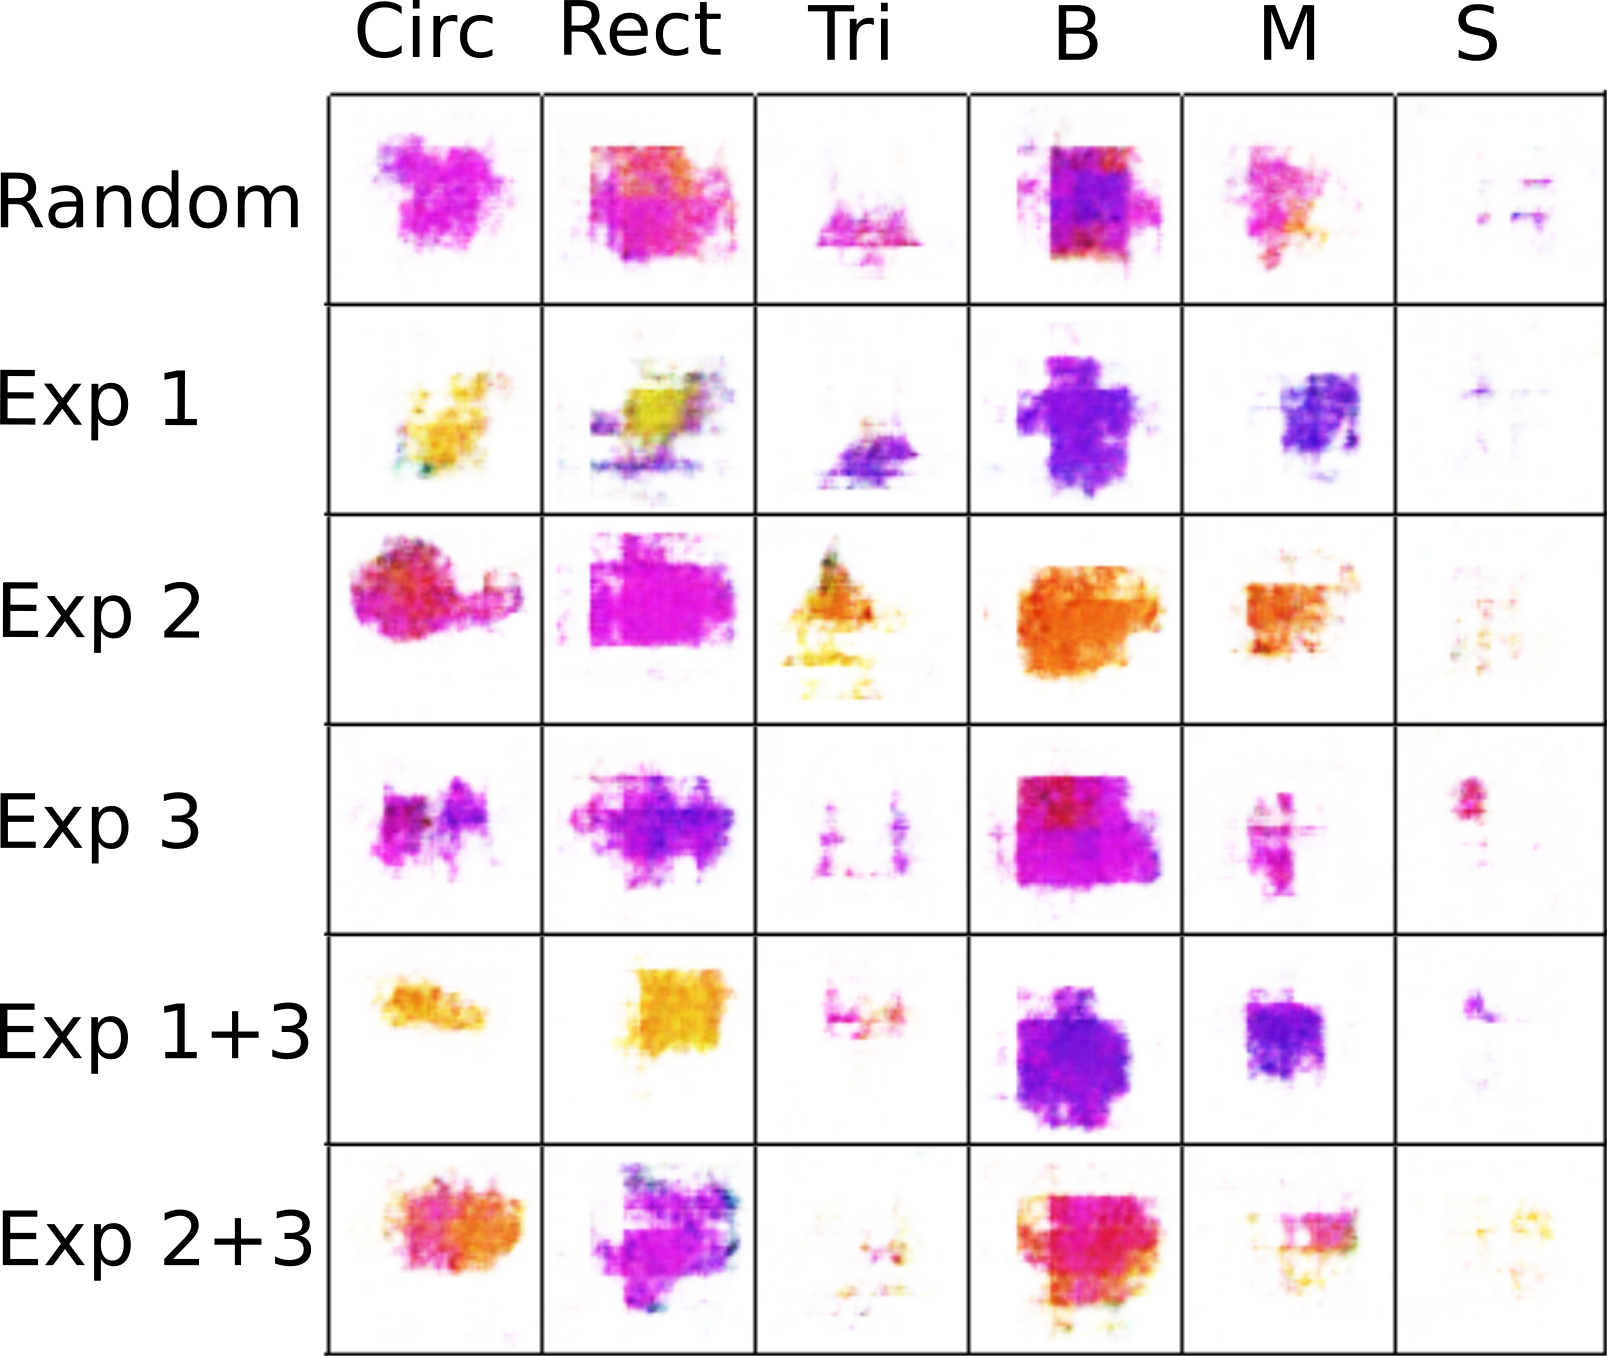
\includegraphics[width=0.75\textwidth]{Figs/shapes/singlelabel739_shape.png}
\caption{Experiment 4, run A: Images generated from shape, and size word for different weight initialisation conditions.}
\label{fig:739single_shape}
\end{figure}



\begin{figure}[h!]
\centering
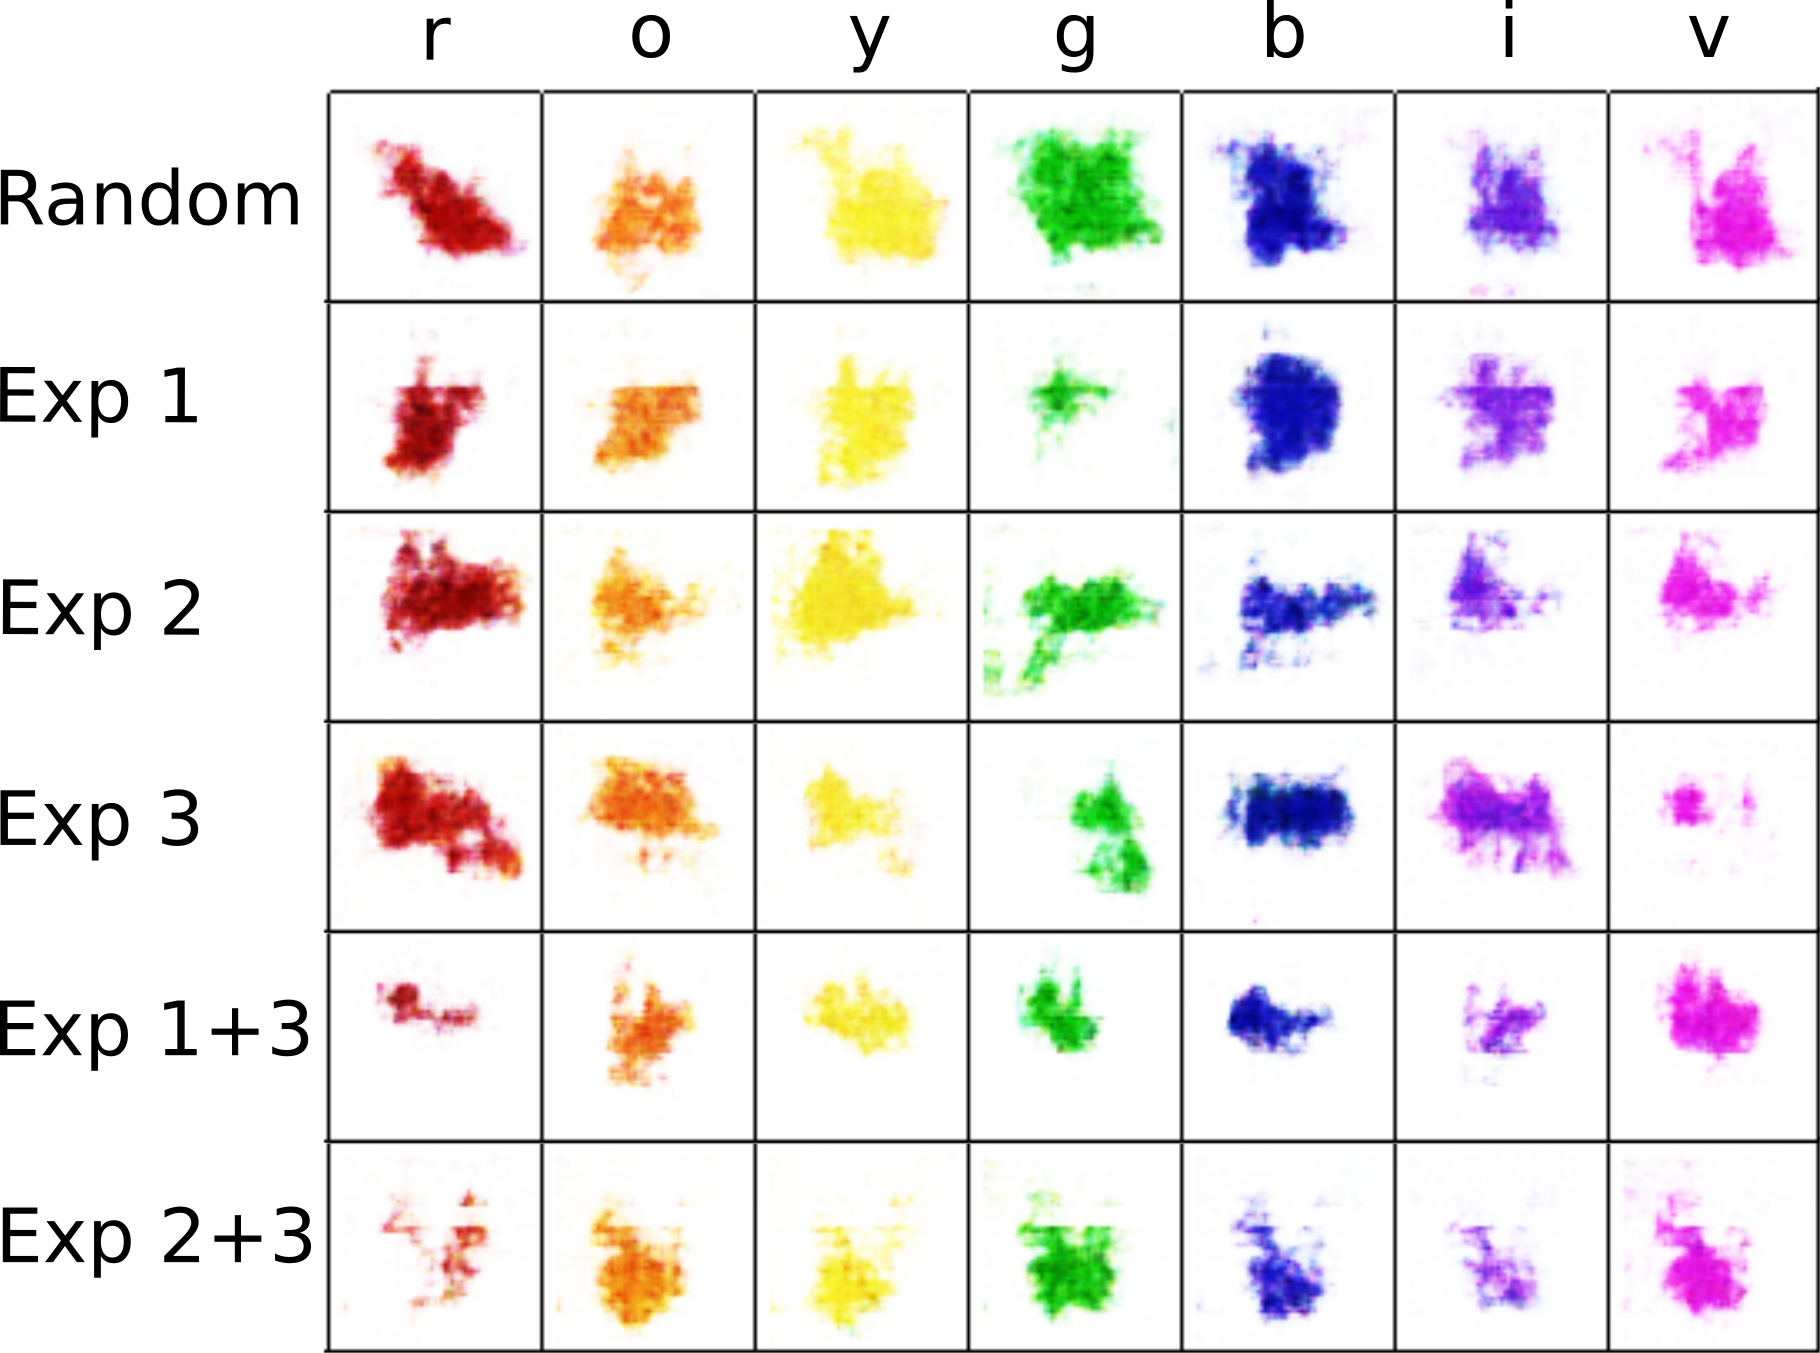
\includegraphics[width=0.75\textwidth]{Figs/shapes/singlelabel739_col.png}
\caption{Experiment 4, run A: Images generated from each colour word for different weight initialisation conditions.}
\label{fig:739single_col}
\end{figure}

\begin{figure}[h]
\centering
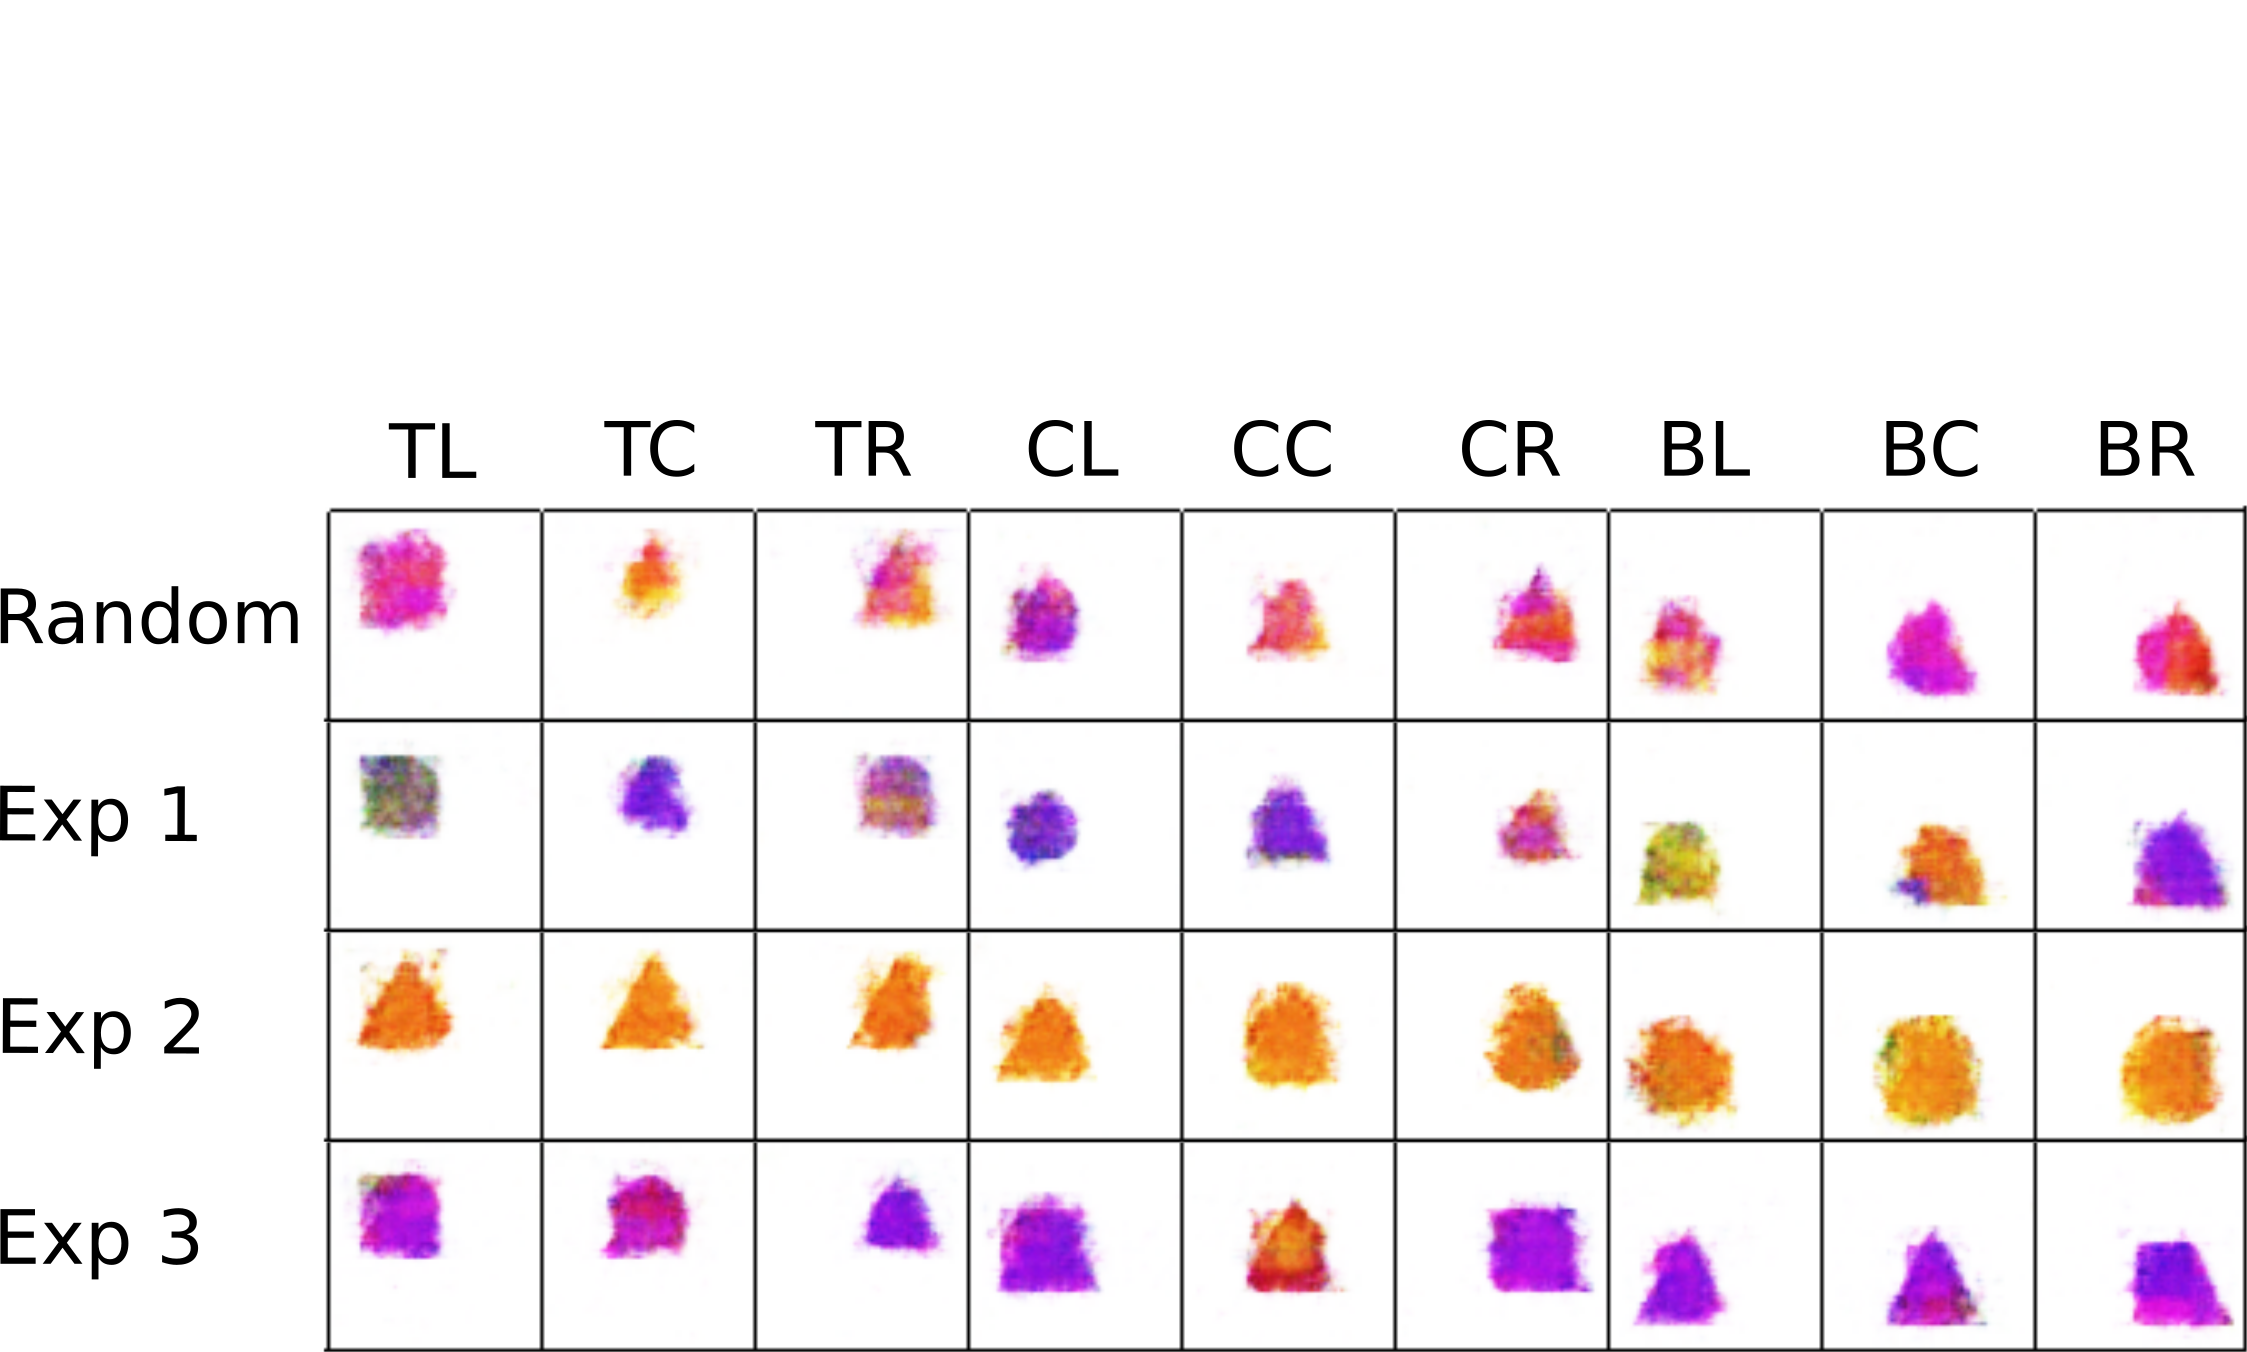
\includegraphics[width=0.75\textwidth]{Figs/shapes/singlelabel739_pos.png}
\caption{Experiment 4, run A: Images generated from each position word for different weight initialisation conditions.}
\label{fig:739single_pos}
\end{figure}

All seven colours are correctly learnt as seen in \autoref{fig:739single_col} for all weight initialisation conditions. As are all 9 positions as seen in \autoref{fig:739single_pos}




\begin{figure}[h!]
\centering
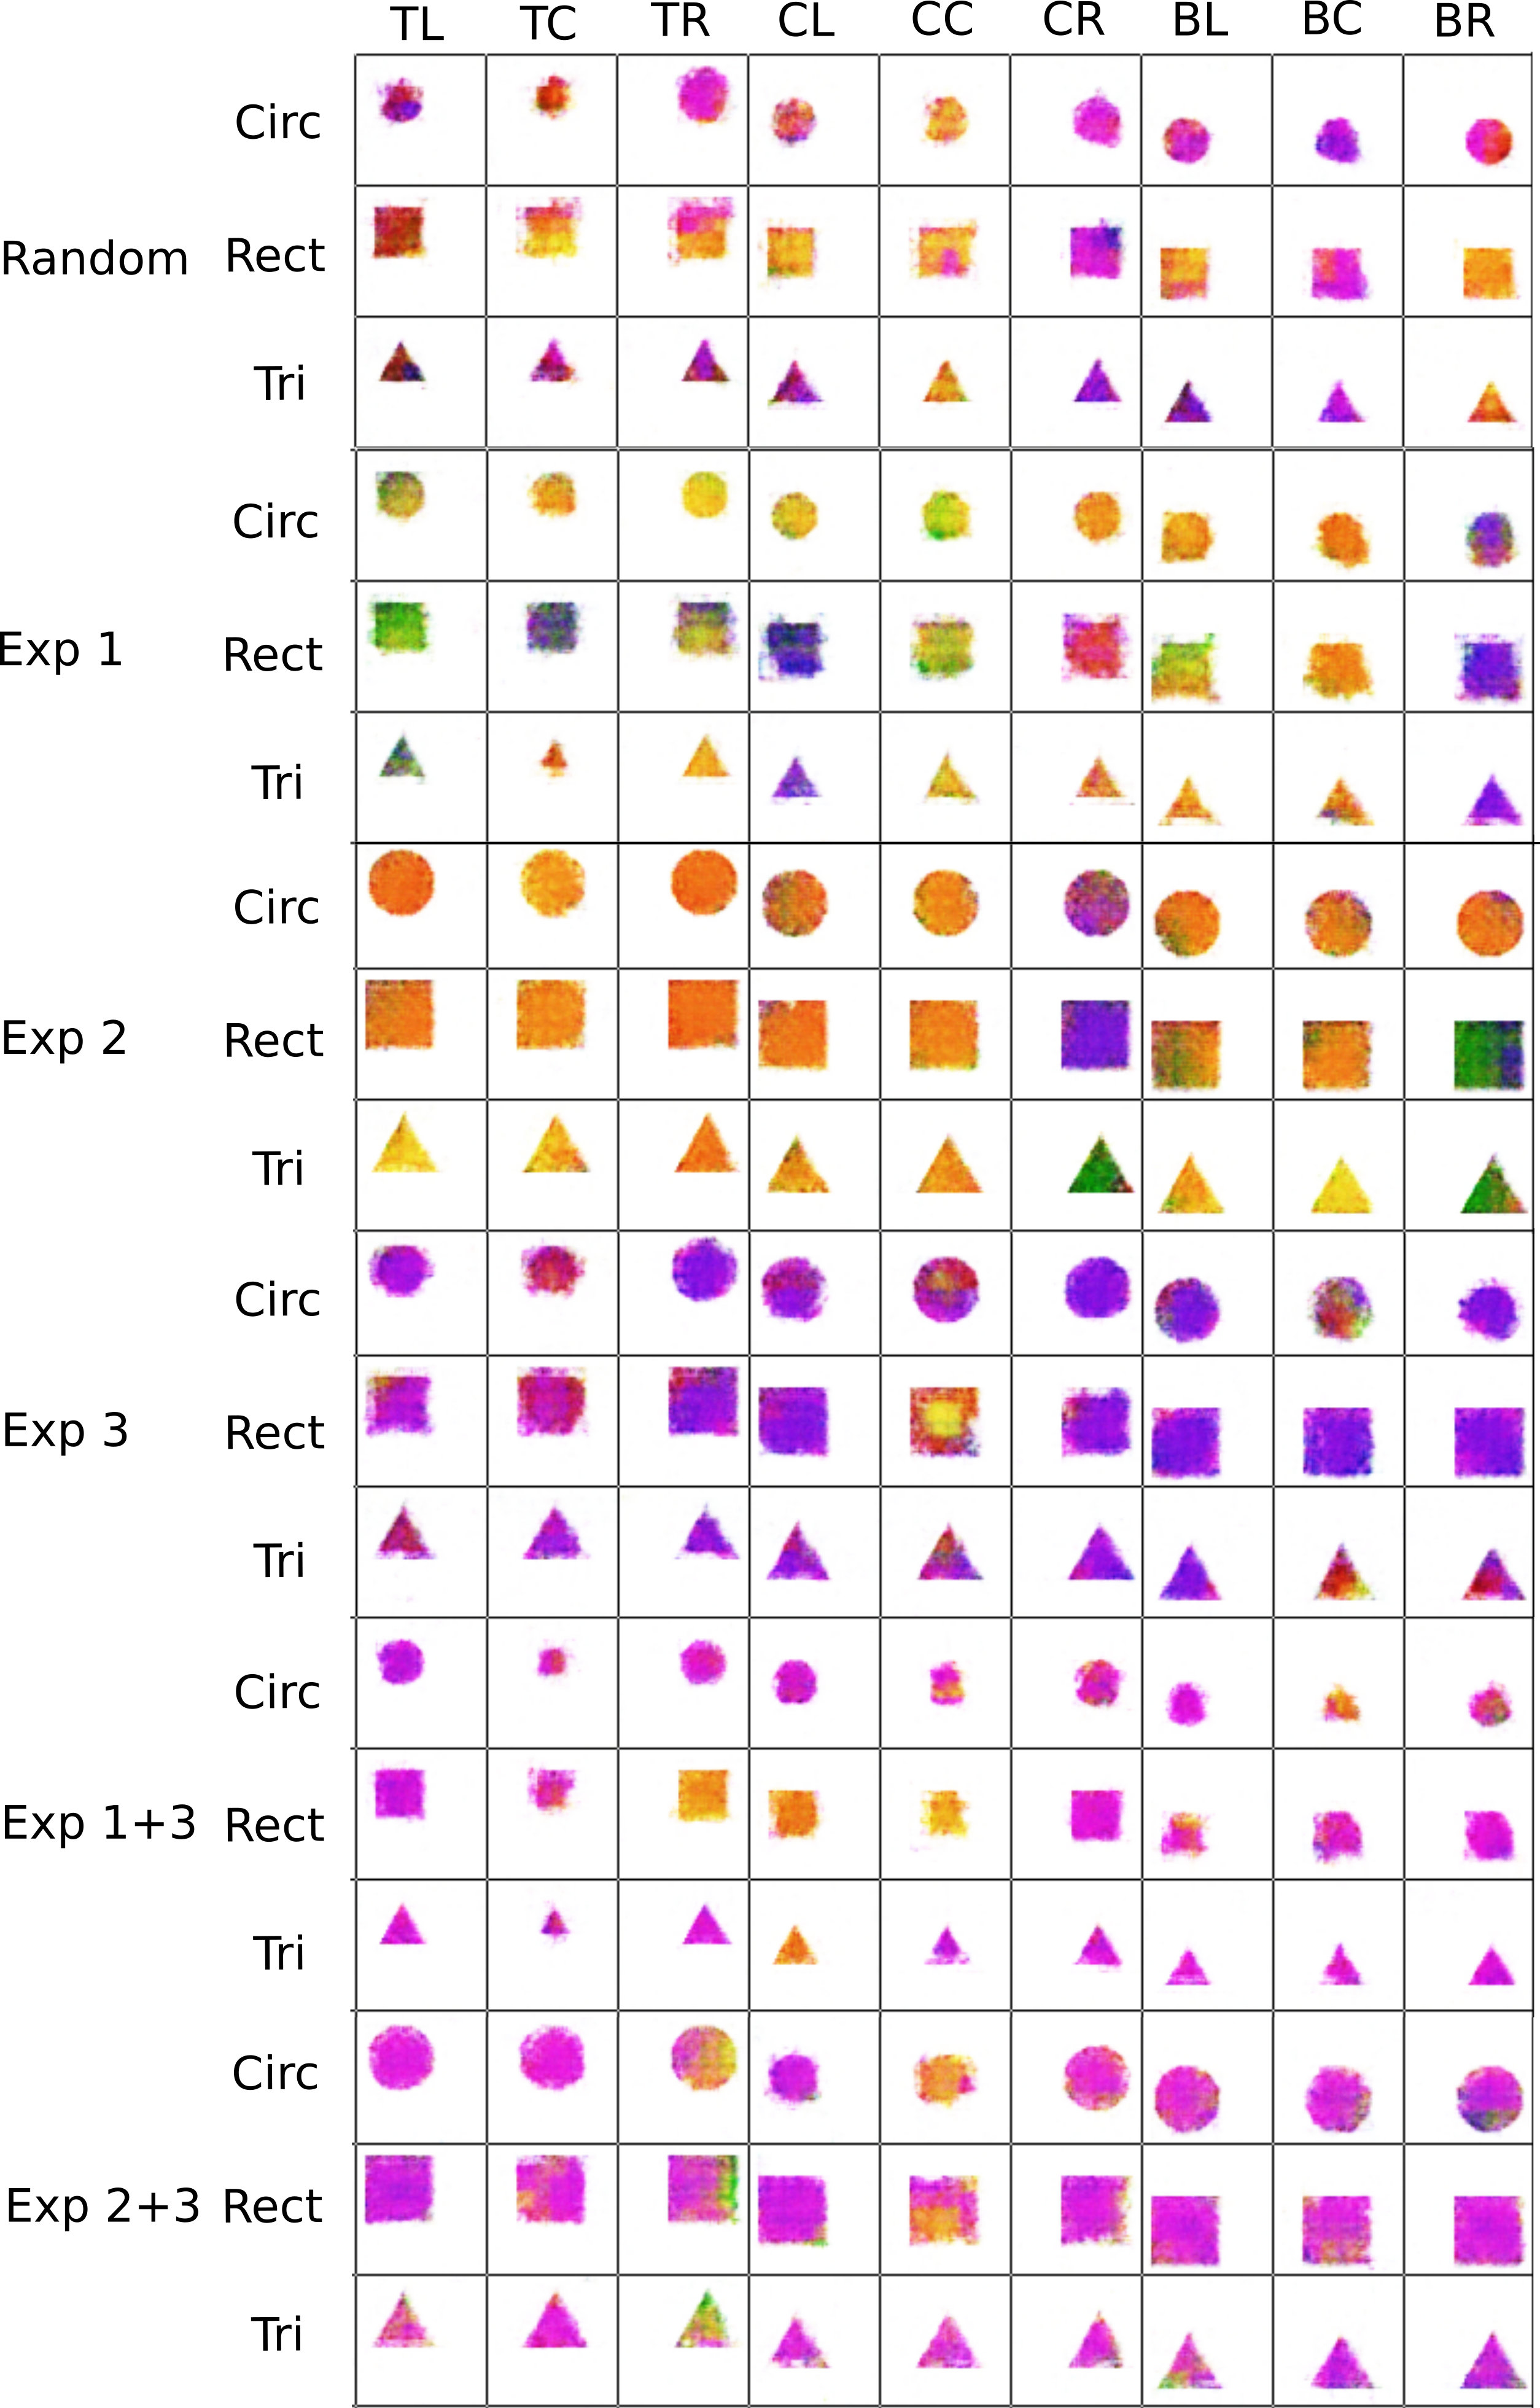
\includegraphics[width=0.75\textwidth]{Figs/shapes/2word739_pos.png}
\caption{Experiment 4, run A: Images generated using word pairs.}
\label{fig:2word739}
\end{figure}

The addition of pretraining has a positive effect on the grounding of the meaning of all words, however this is particularly clear in the case of the shape words, \textsc{Circle}, \textsc{Rectangle} and \textsc{Triangle}. \autoref{fig:2word739} shows that without pretraining, the shapes generated by the \ac{MAE} when two words are given as input (a shape and position) are blurry. For example, generating an image from the words \textsc{Circle, Centre Right} leads to a \textit{Circle} with protrusions in the random initialisation condition, with no clear boundary between the shape and the background.

Pretraining on experiment 2 gave the best results, with all shapes apearing solid and correctly positioned without extraneous edges or protrusions. 

Comparing \autoref{fig:2word739} to the errors in \autoref{tab:res739}, it would be expected that the best image generation to occur when using the \ac{MAE} initalised with weights from experiment 1, however, this suggests that the \ac{MAE} has learnt the meaning of the descriptions as a whole and has not grounded the meanings of the individual words which make up the descriptions.

\paragraph{Description Accuracy}


\begin{table}[h!]
\centering
	\begin{tabular}{|c|c|c|c|}
	\hline
	\textbf{Initialisation} & 	\textbf{Bimodal} & 	\textbf{Image Only} 	& 	\textbf{Words Only} \\ \hline
Random 	&	100.00	$\mypm$	0.00	&	96.10	$\mypm$	6.29	&	100.00	$\mypm$	0.00	\\ \hline
Exp 1	&	100.00	$\mypm$	0.00	&	99.49	$\mypm$	2.21	&	100.00	$\mypm$	0.00	\\ \hline
Exp 2	&	100.00	$\mypm$	0.00	&	\textbf{99.53}	$\mypm$	1.22	&	100.00	$\mypm$	0.00\\ \hline
Exp 3	&	100.00	$\mypm$	0.00	&	99.06	$\mypm$	2.42	&	100.00	$\mypm$	0.00\\ \hline
%Exp 1+3	&	100.00	$\mypm$	0.00	&	98.81	$\mypm$	2.69	&	100.00	$\mypm$	0.00\\ \hline
%Exp 2+3	&	100.00	$\mypm$	0.00	&	97.63	$\mypm$	6.54	&	100.00	$\mypm$	0.00\\ \hline

	\end{tabular}
\caption{Experiment 4: Percentage Description Accuracy for different weight initialisations.}
\label{tab:res739acc}
\end{table}

The addition of more variety of colours to the dataset has had a negative effect on description accuracy in the Image Only testing condition, with a small number of images being mislabelled. The \ac{MAE} initialised with weights from expeirment 2 performed the best with a description generation accuracy of 99.53\% (compared to 99.99\% for the top performing model in experiment 3, 133 incorrectly described images versus only 1 incorrectly described in experiment 3, note that experiment 3 uses less data than experiment 4 hence the large difference between the number of incorrectly descirbed images). In the worst case, when training from scratch, the description accuracy in the Image Only testing condition drops to 96.10\% (1106 incorrectly described images).

Unsurprisingly, the \ac{MAE} initialised with weights from experiment 2 has the best description accuracy in the image only testing condition. Given that, in my opinion, this \ac{MAE} also produces the best images from individual and pairs of words, it is clear that bidirectional grounding has occured in this condition. The \ac{MAE} is able to generate the correct visual attributes from the input words and is also able to correctly describe the visual attributes of images. The 99.49\% and 99.06\% acuracy from pretraining on experiments 1 and 3 respectively equate to 145 and 267 incorrectly described images.

\subsubsection{Discussion}
As in experiment 3 there is a clear positive effect of utilising an incremental approach to grounding the meanings of the words and the visual attributes they equate to. 
When training from random weights, the \ac{MAE} struggles to generate images and descriptions in the Image Only test condition, with a four-fold cross-validated \ac{MSE} that is an order of magnitude worse than the best performing pretrained models. This not only proves hypothesis 4: \ac{MRL} can be improved through transfer learning to be correct, but also demonstrates the importance of taking this approach to achieve the best possible results.

\begin{table}
\centering
\begin{tabular}{|c|c|}
\hline
\textbf{Initialisation} & \textbf{Total Weight Updates}\\ \hline
Random (50 Epochs) &  1,417,500\\ \hline
Random (100 Epochs) & 2,835,000\\ \hline
Exp 1 & 1,485,000\\ \hline
Exp 2 & 1,620,000\\ \hline
Exp 3 &	2,025,000\\ \hline

\end{tabular}
\caption{Experiment 4: Total number of weight updates.}
\label{tab:updatesTotal4}
\end{table}

\begin{table}[h!]
\centering
\begin{tabular}{|c|c|c|c|}
	\hline
	\textbf{Measure} & 	\textbf{Bimodal} & 	\textbf{Image Only} 	& 	\textbf{Words Only} \\ \hline
MSE	&	3.82	$\mypm$	0.12	&	32.58	$\mypm$	36.49	&	4.00	$\mypm$	0.10	\\ \hline
Accuracy	&	100.00	$\mypm$	0.00	&	97.44	$\mypm$	5.77	&	100.00	$\mypm$	0.00\\ \hline
\end{tabular}

\caption{Experiment 4: Mean Squared Error ($\times10^{-3}$) and Percentage Description Accuracy for the randomly initialised MAE after 50 epochs of training.} 
\label{tab:res739_50}
\end{table}

Again, the best performing \ac{MAE} didn't recieve the most training updates. However, the worse performance of the \ac{MAE} initialised with random weights is not only due to overfitting from making too many updates to its weights; after 50 epochs of training, the randomly initalised MAE had poor performance despite only updating its weights 1.4 million times, compared to the 1.6 million updates of the \ac{MAE} initialised with weights from experiment 2. The better performance after 50 epochs  of training compared to after 100 epochs of training suggests that some overfitting has occured (\autoref{tab:res739_50}).



In both experiments 3 and 4, the best performance was seen from the MAE initialised with weights from experiment 2 (Exp 2). It is not obvious why this is. The Exp 2 weights achieved good performance in all testing conditions in experiment 2 (\autoref{tab:res333}). Compare this to the Exp 3 weights, which performed poorly when tested in experiment 3 in the Image Only condition (\autoref{tab:res339}). This suggests that grounding of the visual attributes was not achieved and explains why the \ac{MAE} from experiment 4 initialised with Exp 3 weights does not perform as well as the \ac{MAE} initialised with Exp 2 weights. The \ac{MAE} from experiment 2 had learnt to bidrectionally ground all of the words and visual attributes of the data-subset for experiment 2. The \ac{MAE} from experiment 3 had not learnt to bidirectionally ground all of the words and visual attributes of the data-subset for experiment 3.

Whilst the weights Exp 1 performed well in experiment 1 (\autoref{tab:res331}, they did not perform as well as the Exp 2 weights in experiment 3 (\autoref{tab:res333}) suggesting the qualtiy of the grounding was slightly lower. Further to this, there is a much bigger difference between the types of objects seen by the Exp 1 weights and those seen in experiments 3 and 4, meaning that the \ac{MAE} initialised with the Exp 1 weights has more to learn than the \ac{MAE} initialised with Exp 2 weights.

So, the Exp 2 weights likely lead to the best performance due to 2 factors: 1) the types of objects used to train it are more similar to those used in experiments 3 and 4 compared to those seen by the Exp 1 weights and 2) they have achieved bidirectional grounding of the data-subset of experiment 2, as shown by their superior performance in experiment 2 compared to the Exp 3 weights which did not achieve bidirectional grounding of the data of experiment 3.

\newpage
\subsection{Experiment 5}
In this experiment I select certain subsets of objects from the data to omit, such as violet circles or green triangles. Then I demonstrate how images of these objects can still be generated from their descriptions or through vector arithematic, as well as how images of these objects can be correctly described by the network.

I will examine the omission of 3 different objects, these trials will be referred to as MAE-GT: omission of green triangles, MAE-OR: omission of orange rectangles and MAE-VC: omission of  violet circles. Each MAE is initialised with random weights and trained for 50 epochs.

\subsubsection{Results}

When testing the \acp{MAE} with object types they have seen before (i.e. not objects which were ommited from the training data) the perfomance is similar to that of the randomly initilaised \ac{MAE} of experiment 4 (\autoref{tab:res739_50}). This is to be expected as the data and training setup is identical apart from the omitted objects (\autoref{tab:res_exp5}).

\begin{table}[h!]
\centering
	\begin{tabular}{|c|c|c|c|}
	\hline
\textbf{Trial} & 	\textbf{Bimodal} & 	\textbf{Image Only} 	& 	\textbf{Words Only} \\ \hline
MAE-GT	&	3.87	$\mypm$	0.23	&	43.22	$\mypm$	44.88	&	4.05	$\mypm$	0.24	\\ \hline
MAE-GT*	&	5.21	$\mypm$	0.78	&	86.71	$\mypm$	75.11	&	5.28	$\mypm$	0.55	\\ \hline
MAE-OR	&	3.72	$\mypm$	0.21	&	15.60	$\mypm$	23.65	&	3.97	$\mypm$	0.29	\\ \hline
MAE-OR*	&	4.95	$\mypm$	1.02	&	41.54	$\mypm$	23.46	&	7.18	$\mypm$	2.74	\\ \hline
MAE-VC	&	3.07	$\mypm$	0.77 	&	43.95	$\mypm$	79.53	&	4.12	$\mypm$	0.09	\\ \hline
MAE-VC*	&	4.01	$\mypm$	0.32	&	86.16	$\mypm$	123.74	&	2.67	$\mypm$	0.24	\\ \hline
\end{tabular}
\caption{Experiment 5: Total MSE. Alternating rows show MSE for the datasubset without the omitted data and MSE for only the omitted data (marked with *). (All values are $\times10^{-3}$.)}
\label{tab:res_exp5}
\end{table}

Testing with only the omitted object, there is an increase in \ac{MSE}, particularly for the Image Only testing condition. This is to be expected as the MAE has never seen these objects before, and will therefore be biased towards generating outputs which are more simlar to its training data than those required to perform well at generating the correct output for the omitted objects (\autoref{tab:res_exp5}).


\paragraph{Image Generation}
To further demonstrate the abilities of multimodal representation learning through the use of \acp{MAE}, I used three subsets of data to train three \acp{MAE}. Each of the MAEs was trained 4 times for validation purposes as with all other experiments, the mean result for the four runs is presented.

For each training subset, a shape of a particular colour was omitted from the training data. In \autoref{fig:739_minus1}, \acp{MAE} 1, 2 and 3 were trained without green triangles, orange rectangles and violet circles, respectively. Generating images from full descriptions still results in correctly generating images of green triangles, orange rectangles and violet circles, showing that each \ac{MAE} has learnt the meaning of these words individually and hence can ``imagine'' what their combinations should look like. 

\begin{figure}[h]
\centering
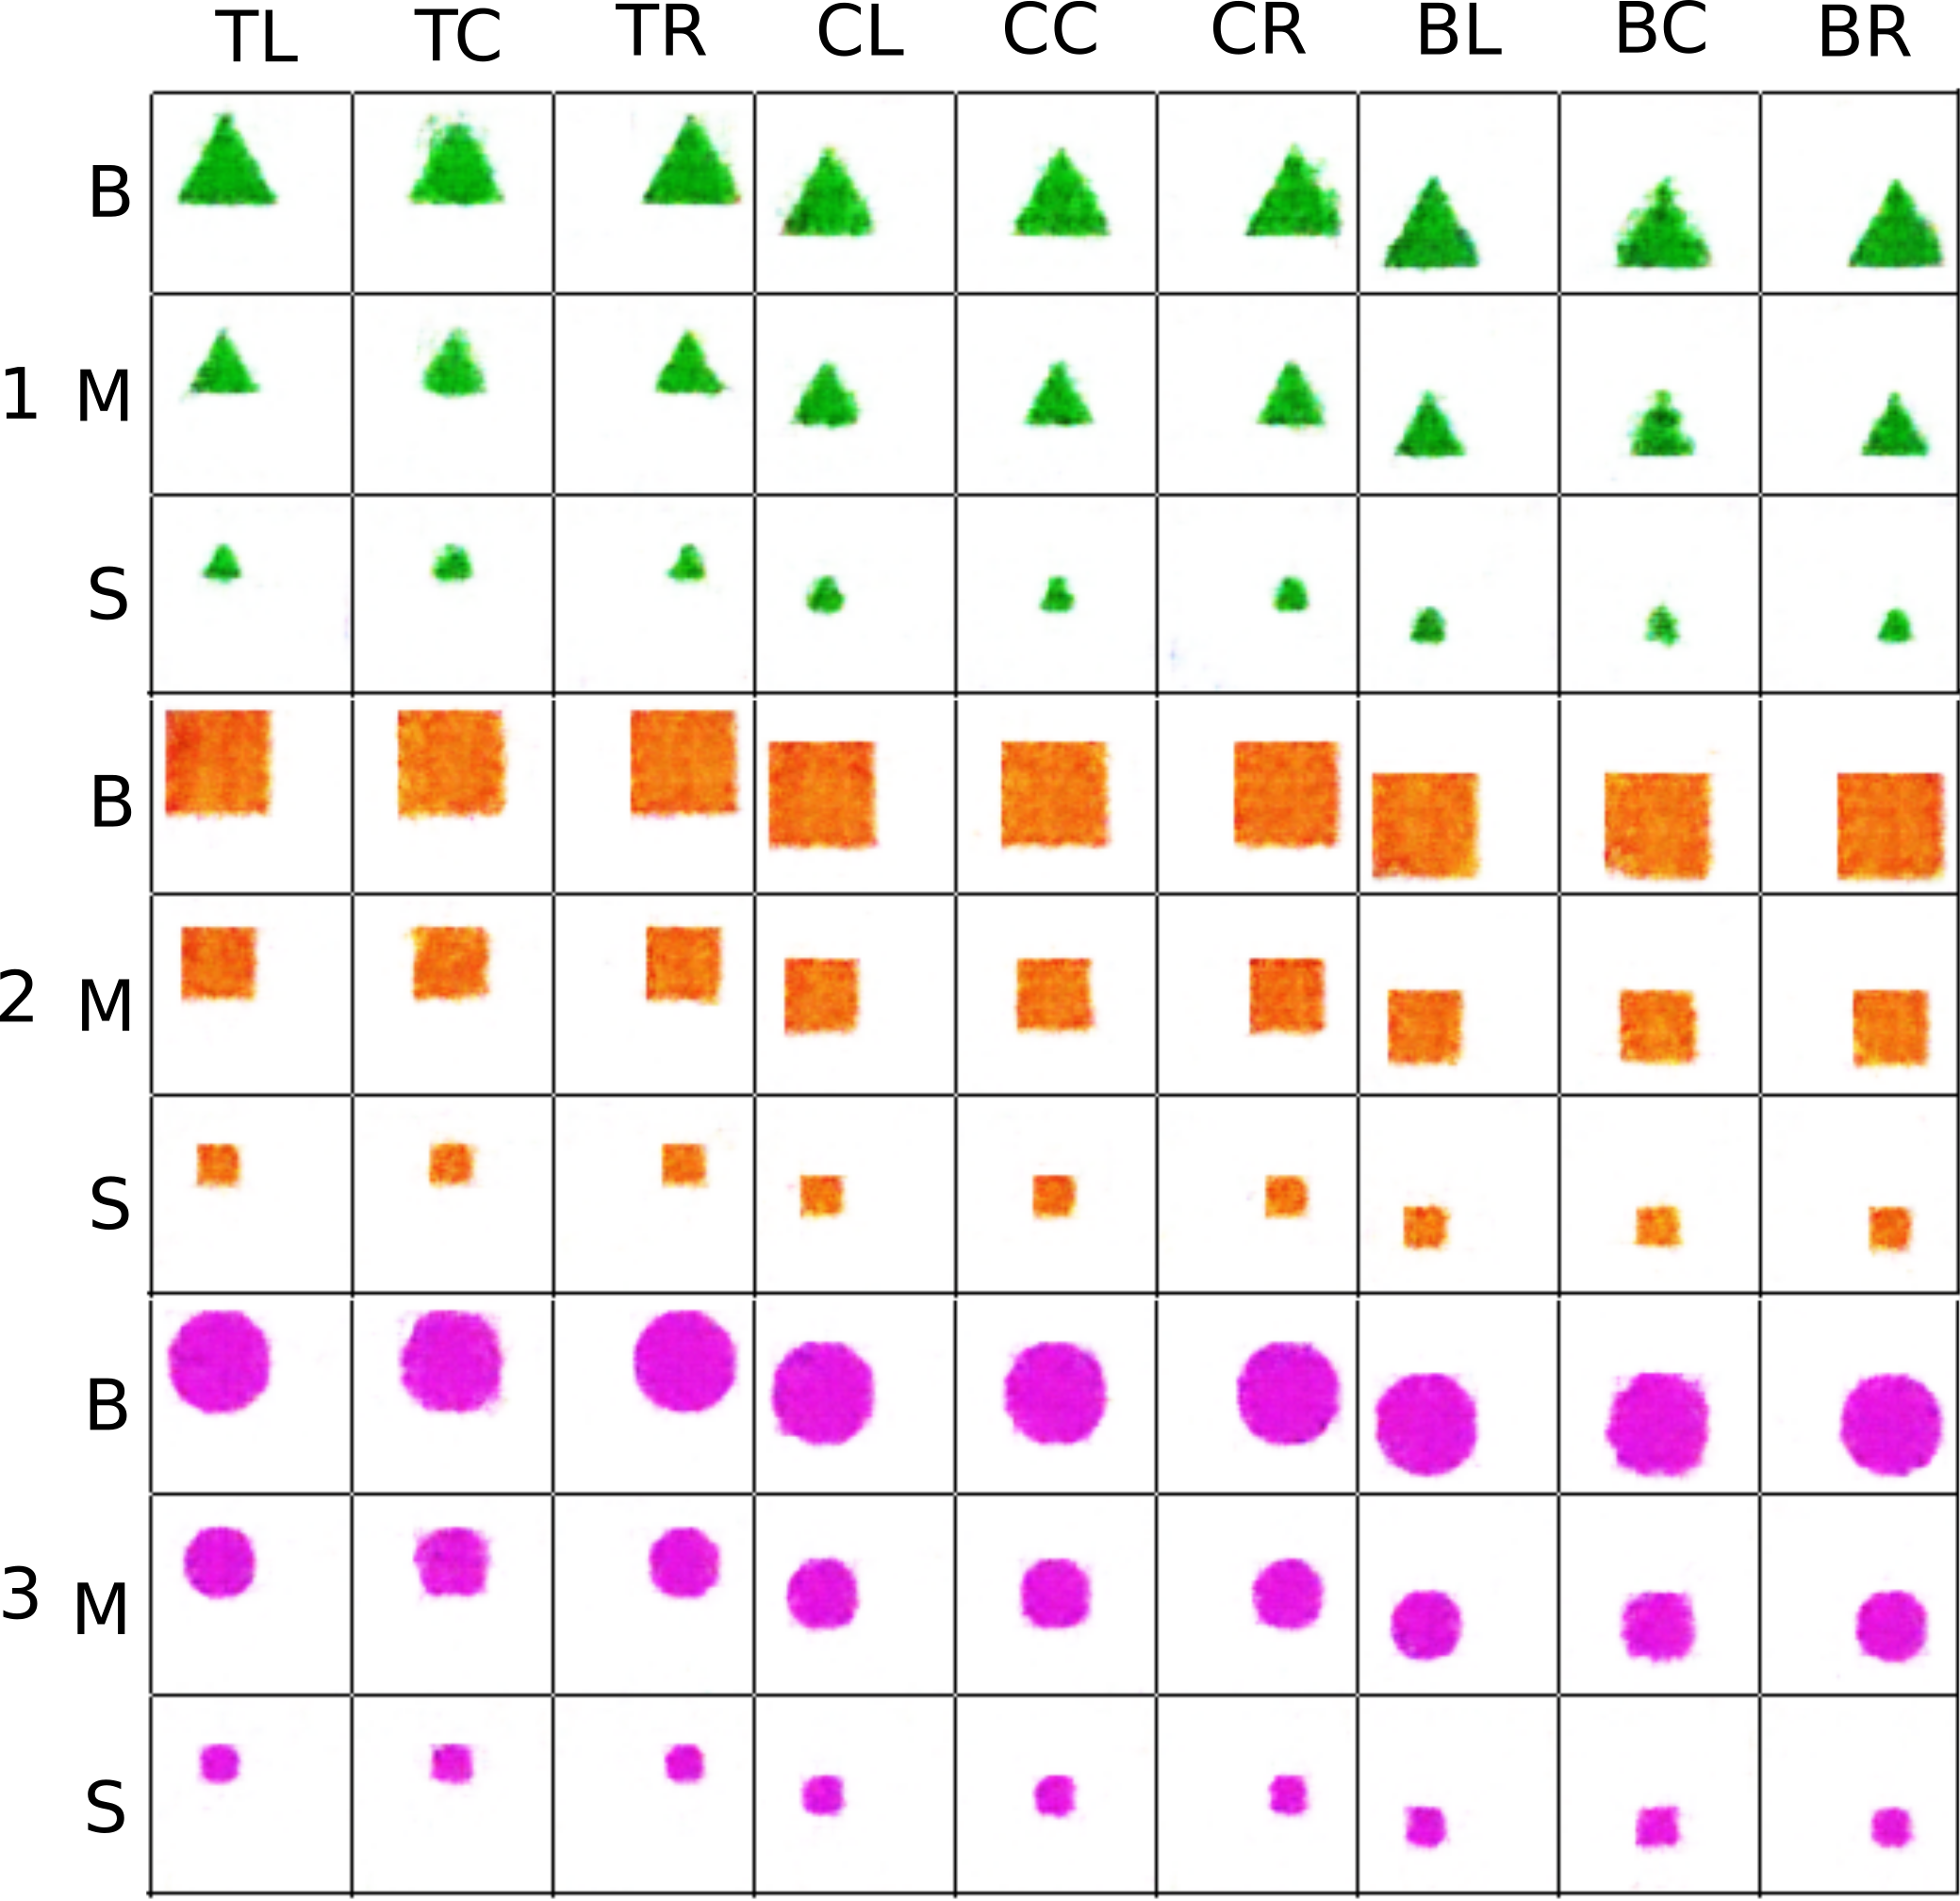
\includegraphics[width=0.7\textwidth]{Figs/shapes/739_minus1.png}
\caption{Experiment 5, run A: Images generated from descriptions of shapes never seen by the \ac{MAE}.}
\label{fig:739_minus1}
\end{figure}

Despite never seeing a green triangle, \ac{MAE} 1 from \autoref{fig:739_minus1} has learnt the meaning of each of the words \textsc{Triangle} and \textsc{Green} from instances of other coloured triangles and green circles and rectangles. A similar statment can be made about \acp{MAE} 2 and 3 in \autoref{fig:739_minus1}.

\begin{figure}[h]
\centering
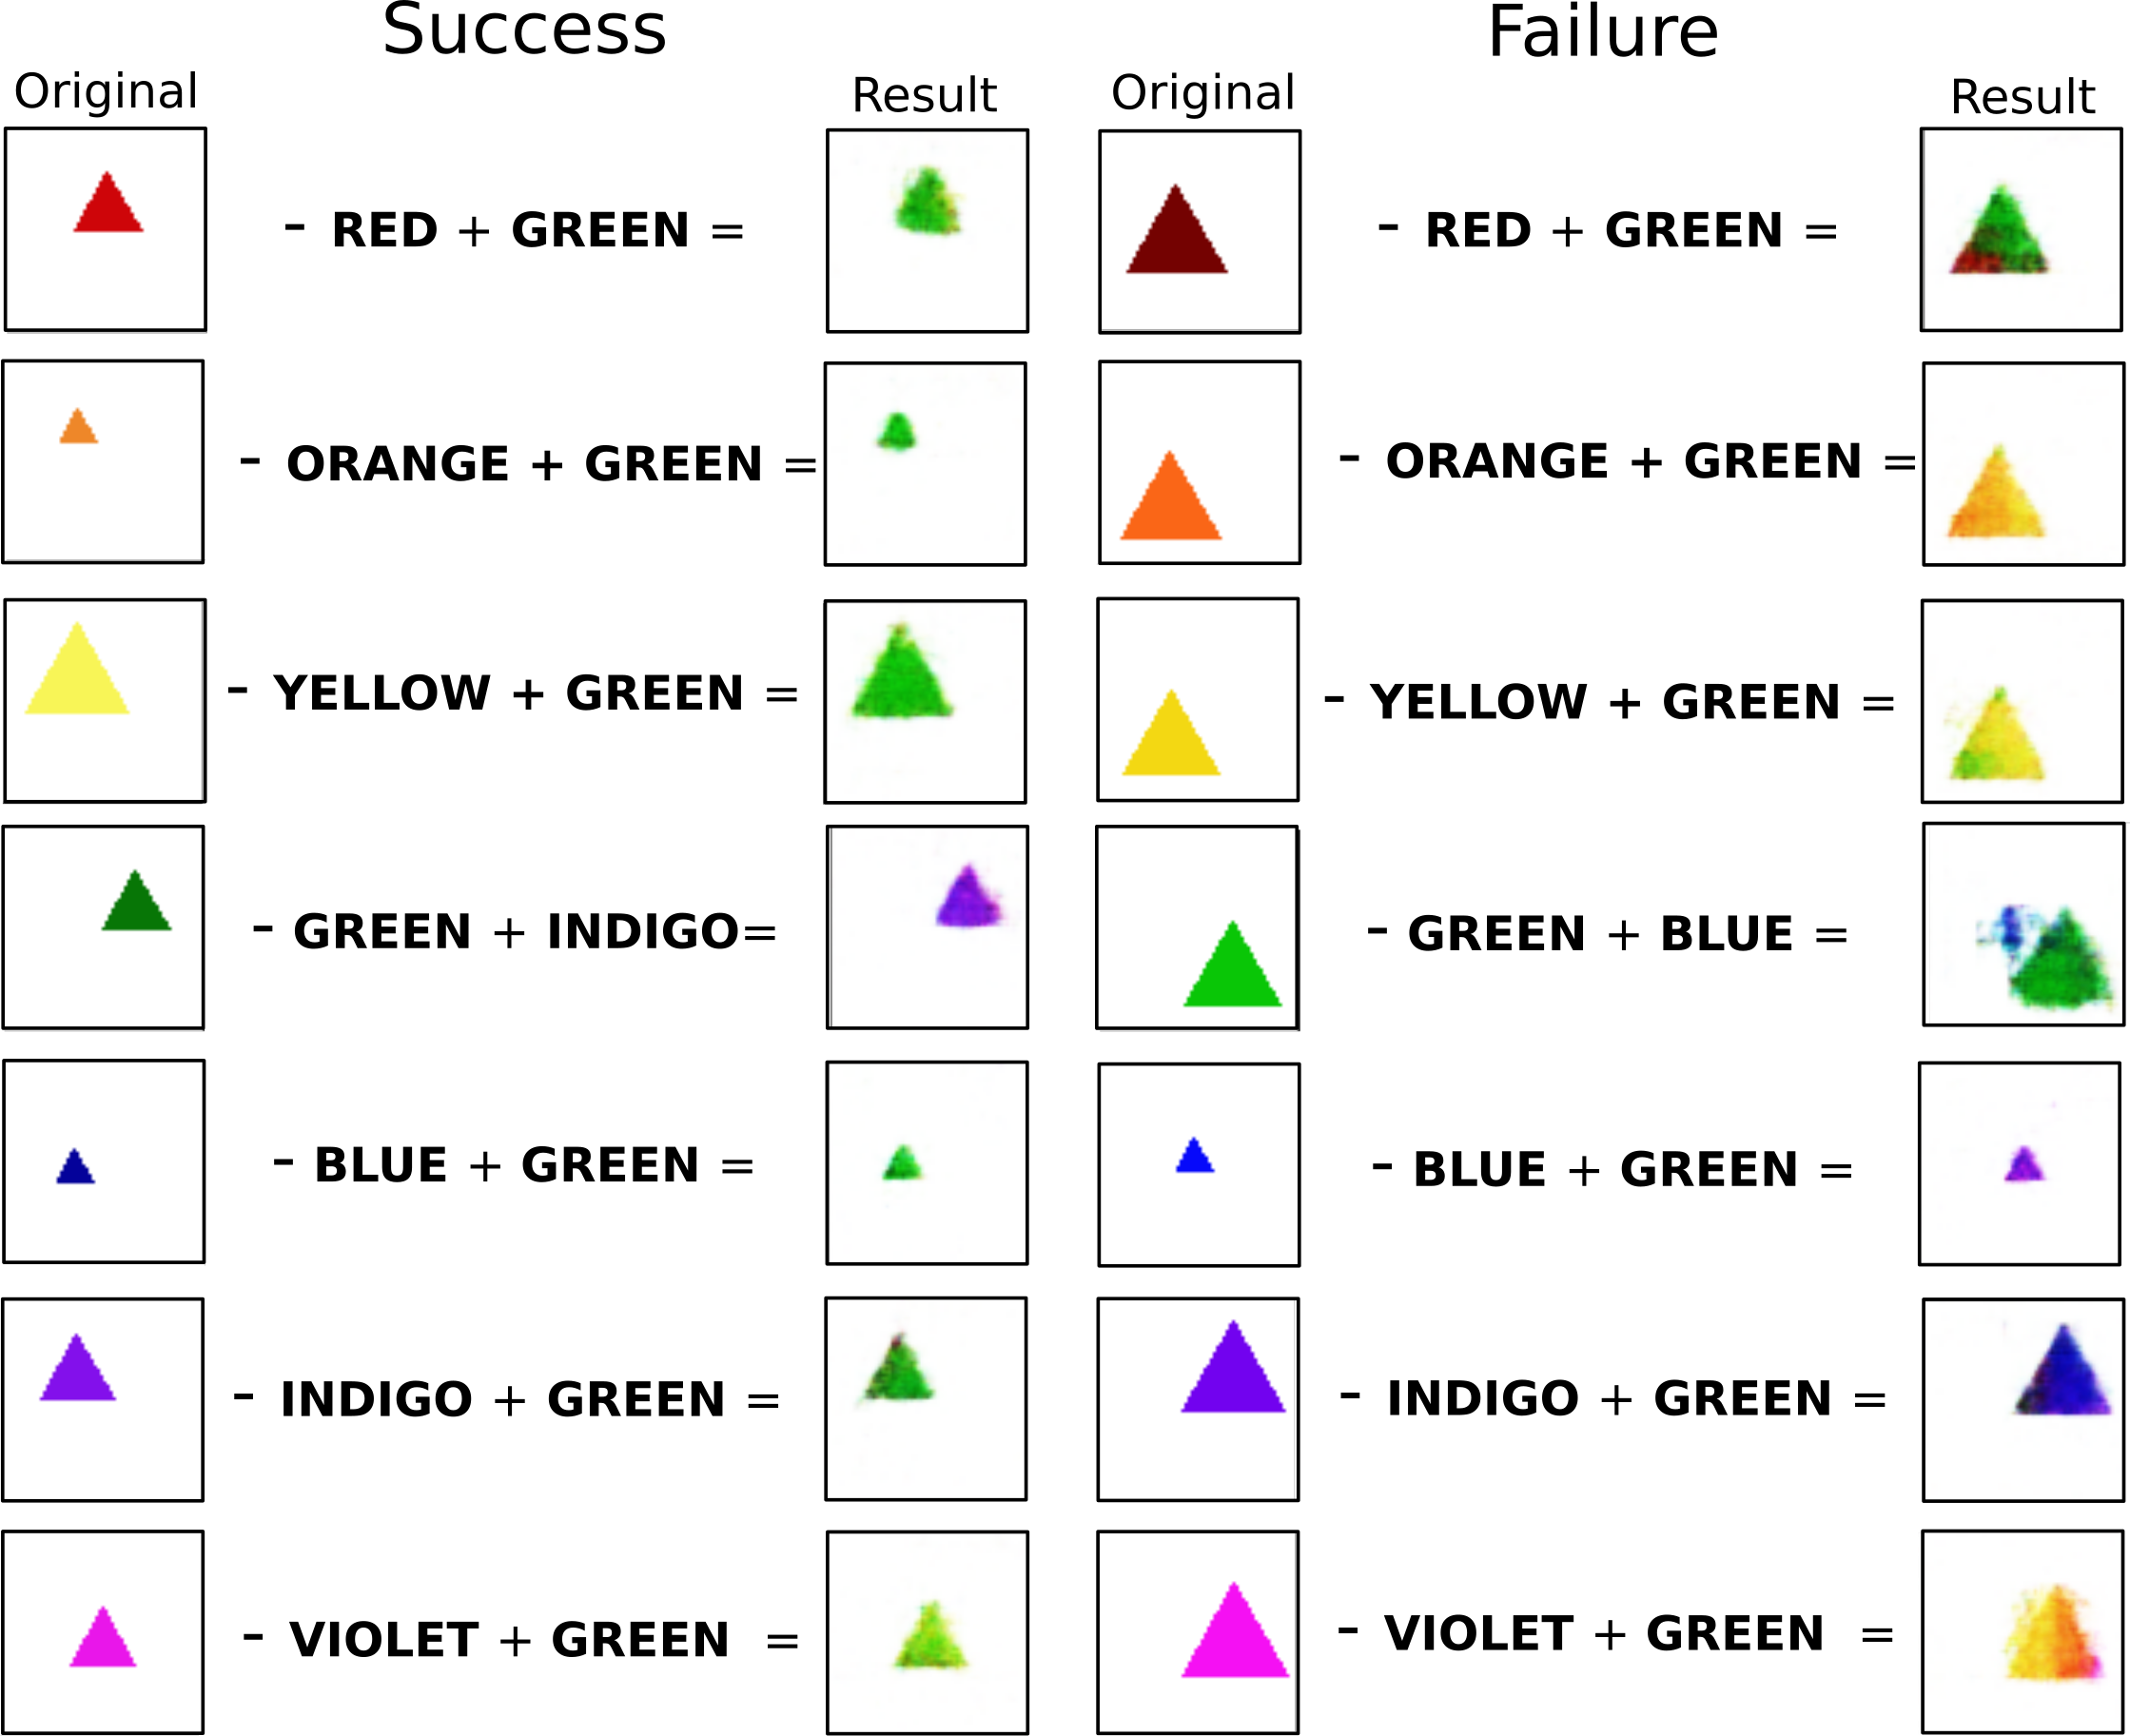
\includegraphics[width=0.75\textwidth]{Figs/shapes/739_minus1_vectorArthGT.png}
\caption{Experiment 5, run A: Images generated via Vector Arithmetic by MAE-GT.}
\label{fig:739_vectorArth}
\end{figure}

As explained earlier in this chapter, it is also possible to generate novel images by manipulating the embedding space of the \ac{MAE} via Vector Arithmetic. \autoref{fig:739_vectorArth} shows a sample of images generated by \ac{MAE} 1 (Results for \acp{MAE} 2 and 3 are in the supplemental material).

Whilst some manipulations are successful for \ac{MAE} 1, not all are. This is likely due to discontinuities in the latent embedding space. As the \ac{MAE} has not been trained on every possible combination of colours, sizes, shapes and positions, there are parts of the embedding space it has never trained. This means that when vector arithmatic creates an embedding which lies in one of these unexplored areas, the \ac{MAE} will not generate a sensible output. 

This demonstrates that the representation learnt by the \ac{MAE} does fulfil some of the criteria laid out by Bengio et al. \cite{repRev} as the representation of each individual visual attribute maintains its meaning even in unseen combinations of visual attributes. However, the learnt representation does not fulfil all of these criteria due to the discontinuities in the latent space. In order to accept hypothesis 5: the multimodal representation learnt by the \acp{MAE} exhibits all of the desirable properties of a representation as layed out by Bengio et al. in \cite{repRev}, it will be necessary to find methods to remove these discontinuites. Possible approaches to this would be the addition of either a variational cost \cite{kingma2013auto} or vector quantisation \cite{wavenet} on the latent space. I chose not to implement such a constraint, as I deemed that it would place an unfounded constraint on the embedding of the \ac{MAE}. However, a future experiment would validate whether or not my choice was correct.

\paragraph{Description Accuracy}
\begin{table}[h!]
\centering
	\begin{tabular}{|c|c|c|c|}
	\hline
\textbf{Trial}	 & 	\textbf{Bimodal} & \textbf{Image Only} 	& 	\textbf{Words Only} \\ \hline
MAE-GT	&	99.99	$\mypm$	0.05	&	96.86	$\mypm$	7.10	&	100.00	$\mypm$	0.00	\\ \hline
MAE-GT*	&	99.98	$\mypm$	0.10	&	92.54	$\mypm$	13.30	&	100.00	$\mypm$	0.00	\\ \hline
MAE-OR	&	100.00	$\mypm$	0.00	&	99.03	$\mypm$	3.57	&	100.00	$\mypm$	0.00	\\ \hline
MAE-OR*	&	99.97	$\mypm$	0.17	&	96.31	$\mypm$	10.065	&	99.68	$\mypm$	16.41	\\ \hline
MAE-VC	&	100.00	$\mypm$	0.02	&	96.54	$\mypm$	7.71	&	100.00	$\mypm$	0.00	\\ \hline

MAE-VC*	&	99.95	$\mypm$	0.32	&	92.27	$\mypm$	17.55	&	100.00	$\mypm$	0.00	\\ \hline

	\end{tabular}
\caption{Experiment 5: Percentage Description Accuracy. Alternating rows show accuracy for the datasubset without the omitted data and MSE for only the omitted data (marked with *).}
\label{tab:res_exp5_acc}
\end{table}

The \acp{MAE} are still able to accurately describe images of objects which appeared in the training data. However, they are also able to describe the images of the objects which were omitted from the training data. The \acp{MAE} have grounded the meanings of the all visual attributes, regardless of having some combinates excluded from the training data (e.g. green triangles). There is an overall decrease in description accuracy for the omitted objects ($\approx 96 \% --> \approx 92 \%$). However for the non-omitted objects the performance is comparable to the accuracy of the random condition from experiment 4.


\subsection{Discussion}
Omitting one object from the training data has a minimal effect on the reconstruction of the other objects in the dataset, this can be seen by comparing the random initialisation condition from \autoref{tab:res739} and the results shown \autoref{tab:res_exp5}. This means that omitting one object, such as green triangles, does not affect the ability of the \ac{MAE} to learn to ground the visual attributes \textit{Green} and \textit{Triangle} nor the words \textsc{Green} and \textsc{Triangle}. It can still generate green objects and triangles, approximately as well as the randomly initalised MAE from experiment 4.

This is further demonstrated by the \acp{MAE} ability to generate images of the unseen objects as shown in \autoref{fig:739_minus1}. As the \ac{MAE} has grounded the meanings of the visual attributes \textit{Green} and \textit{Triangle} and the words \textsc{green} and \textsc{triangle}, it is able to combine their meanings to generate images of green triangles in different positions and sizes. (This is also true for orange rectangles and violet circles).

There is a negative effect on the reconstruction error for the ommited object and the labelling of the omitted object also suffers. Whilst labelling accuracy for objects types included in the training data generally remained very good (over 96\% in the image only testing condition), labelling of the omitted object was noticably worse, with an average of a 3.61\% reduction in accuracy across the three omitted objects. This means that only approximately 378 out of 9450 images, of each object which has been seen, are incorrectly described (9450 = 9 positions x 7 colours x 3 sizes x 50 samples). Compare this, to approxiamtely 103 out of 1350 unseen objects incorrectly classified (1350 = 9 positions x 1 colour x 3 sizes x 50 samples)

Seeing that both accurate descriptions and reconstructed images can be generated by the \ac{MAE} for unseen objects, I can conclude that the \ac{MAE} is capable of bidirectional symbol grounding. This also highlights the effectivness and utility of this method. There is not a decrease in performance compared to the random condition of experiment 4, it is therefore possible that the \ac{MAE} can be used to accuartely label unseen objects without a decrease in performance on seen objects.


\subsubsection{How an incremental approach helps}
It might seem that the task of learning to bidirectionally ground the words of the descriptions and the visual attributes of the images is trivial. Of course, it is for an adult human. Even if the descriptions were given in an unknown language, given very few examples (possibly even less than one example per object) an adult could learn the relationship very quickly. Why then, does a \ac{ANN} need so many examples to get things right?

The root of this issue comes down to two main factors, 1) the underlying probability distribution of the data and 2) the learning method: gradient descent.

To understand what I mean by ``the underlying probability distribution of the data'' let us consider the simple example of rolling a die to decide if it is fair.

How many times should I roll the die before I decide if it is fair? If it is a six sided die and it is fair, there should be a $\frac{1}{6}$ chance of rolling each of the numbers 1 to 6. So if I roll it 6 times I should expect to see each number once. However, I most likely won't, but that doesn't mean the die is rigged.

As I roll the die more and more times, I can get a better understanding of the true probability of rolling a given number and therefore get closer to deciding if the die is indeed fair.

\begin{table}[h]
\centering
	\begin{tabular}{|c|c|c|c|c|c|c|}
	\hline
	\textbf{Rolls} & \textbf{1} & \textbf{2} & \textbf{3} & \textbf{4} & \textbf{5} & \textbf{6} \\ \hline
	10 & 0 & 0.2 & 0.2 & 0.3 & 0.2 & 0.1 \\ \hline
	1000 & 0.168 & 0.148 & 0.169 & 0.174 & 0.172 & 0.169  \\ \hline
	100000 & 0.166 & 0.166 & 0.167 & 0.168 & 0.165 & 0.167  \\ \hline
	1000000 & 0.167 & 0.167 & 0.167 & 0.167 & 0.167 & 0.167  \\ \hline
	\end{tabular}
	\caption{Probability distributions generated from rolling a 6 sided die.}
	\label{tab:dieProb}
\end{table}

As I roll the die more and more I will get closer to the actual probability distribution which governs its behaviour. In the limit, the probability for rolling any number should converge to $\frac{1}{6} = 0.167$. Looking at \autoref{tab:dieProb} it can be seen that the \ac{PRNG} I used to simulate rolling a die on my computer, is mostly fair. 

So, how does this relate to the ArtS dataset? Let us replace rolling a die in this example with selecting random images from the ArtS dataset and ask, how much information does a set of samples tell us about the underlying distribution of the dataset. As I can only select a finite number of images, I cannot capture the entire underlying distribution of the data. Therefore when I train an \ac{ANN}, it will have an inaccuracte idea of the cost landscape.

Given how gradient descent works, as explained in \autoref{Chapter3},  minimising the cost until it reaches a minimum, if the \ac{ANN} has an incomplete picture of the cost landscape, it is likely that gradient descent will get stuck in a local minimum, and not find the global minimum.

As it isn't feasible to provide infinite training examples to allow the \ac{ANN} to get a complete picture of the cost landscape, it is necessary to find a way of constraining the cost landscape instead.

Let us consider two scenarios, 1) I sample data for a relatively complex task (like in experiment 4) and start from random weights, 2) I pretrain on a simpler task, then sample data for the more complex task (like in experiment 4 training from the weights learnt in experiment 2).

If I draw the cost landscapes in these two scenarios as well as the true cost landscape, I might get a figure like \autoref{fig:localminima}. The ``sampled cost'' relates to starting from random weights and the ``pretrained cost'' is the estimated cost landscape based on the data seen during pretraining.
\begin{figure}[h!]
\begin{center}
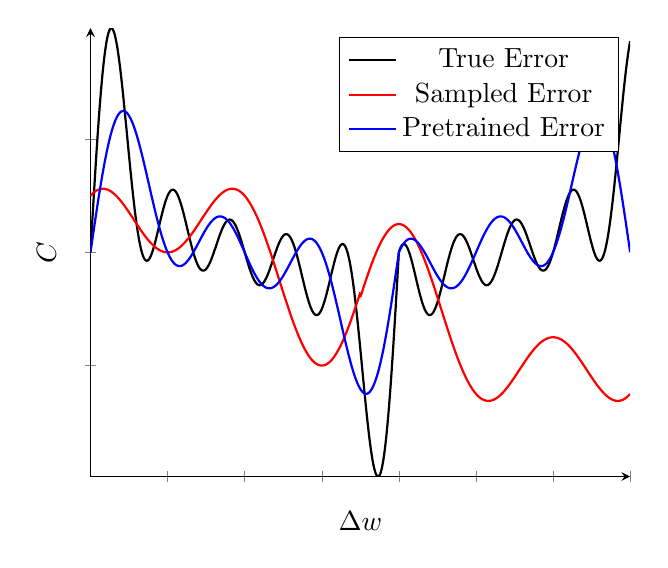
\begin{tikzpicture}
\begin{axis}[
axis lines=left,
xtick={90, 180, 270, 360,450,540,630},
xticklabels={},
xlabel={$\Delta w$},
ylabel={$C$},
yticklabels={},
xlabel near ticks,
ylabel near ticks]
\addplot[black, thick, smooth, samples=1000, domain=0:360]{sin(x) + sin(2*\x)+sin(3*\x)+sin(4*\x) + sin(5*\x)};

\addplot[black, thick, smooth, samples=1000, domain=360:630]{-sin(1*(\x-300)) -sin(2*(\x-300)) -sin(3*(\x-300)) -sin(4*(\x-300)) -sin(5*(\x-300))};




\addplot[red, thick, smooth, samples=1000, domain=0:315]{-cos(1*(\x-270)) -cos(2*(\x-270)) };

\addplot[red, thick, smooth, samples=1000, domain=315:630]{(-cos(\x-180) + -cos(2*\x-180))-1.50};


\addplot[blue, thick, smooth, samples=1000, domain=0:360]{sin(x) + sin(2*\x)+sin(3*\x)};

\addplot[blue, thick, smooth, samples=1000, domain=360:630]{-sin(1*(\x-270)) -sin(2*(\x-270)) -sin(3*(\x-270))};


\node [red] at (470,130)  (a) {\textbullet};
\node [black] at (335,5)  (a) {\textbullet};
\node [blue] at (320,145) (b) {\textbullet};
\legend{True Error, , Sampled Error, , Pretrained Error, }
\end{axis}
    

\end{tikzpicture}
\caption{Visualisation of an imaginary Cost landscape.}
\label{fig:localminima}
\end{center}
\end{figure}

Consider the red point on the red line shown in \autoref{fig:localminima}, this represents the minimum of the cost landscape estimate from sampling data for a task without performing pretraining on a simplier task. It is possible that the weights of the neural network will get stuck in the local minima. This is essentially over fitting the data due to having an unconstrained search space and limited knowledge of the cost landscape.

If I pretrain, allowing the network to first master a simpler task, the estimate of the true cost landscape will be different as it is based off of the data sampled in the simpler task. In \autoref{fig:localminima} this is represented by the blue line. As the \ac{ANN} performs well on the simpler task, it is likely the weights of the network are relatively close to the global optimum before training on the data sampled for the more complex task.


When I pretrain using a different subset of the data as in experiments 3 and 4, the \ac{ANN} starts at a point in the cost landscape that is hopefully closer to the global minima than starting with randomly selected weights. Obviously, this is not always the case, for example, only pretraining on experiment 2 helped in both experiments 3 and 4. Pretraining on experiment 1 did not have a positive effect on the bidirectional symbol grounding.

So, by taking a incremental approach, mastering simple tasks and increasing the difficulty of the tasks we set our  \acp{ANN} to tackle, we can incrementally approach the global cost minima. In the case of the ArtS dataset this means incrementally learning to perform bidirectional symbol grounding on a wider variety of words and visual properties; learning new colours, shapes, sizes and positions. As we saw from the results of experiment 4, this approach can lead to better performance than simply training longer on the more difficult task.

This lines up well with how humans learn \cite{webb2015mother, fantz1963pattern, reid2017human}. We master simple tasks and build upon our existing skills to tackle more difficult problems.

\section{Summary}
This chapter focused on demonstrating how a more complex internal representation could be created and exploited.

I have demonstrated that by utilising a \ac{MAE}, it is possible to learn a multimodal representation of images and their descriptions proving hypothesis 3. The embedding of images or descriptions into this representation can be used to generate novel descriptions or images.

The use of an incremental approach to learning the visual attributes and vocabulary of the ArtS dataset through transfer learning lead to improved bidirectional symbol grounding proving hypothesis 4. This also highlights the ``semi-supervised learning'' and ``shared factors across tasks'' properties of the learnt representation \cite{repRev}. Demonstrating that the representation fulfils some of the criteria for proving Hypothesis 5.

It is possible to directly manipulate the latent representation using vector arithmetic on embeddings from either modality making meaningful changes, generating images with altered visual attributes. Whilst this demonstrates that the learnt representation does fulfil some of the criteria laid out in \cite{repRev} for what makes a good representation, I was unable to accept hypothesis 5. As there are areas of the latent space which do not meet these criteria, hence the generation of incorrect images through vector arithmetic seen in \ref{fig:739_vectorArth}, demonstrating that the representation is not entirely smooth, which is one of Bengio et al.'s criteria for a good representation.

The learnt representation is very robust, even allowing for the generation of unseen combinations of words as images, or the descriptions of images of unseen objects. However, the quality of the representation is highly dependent on the data used for training and the training method used. The best results were achieved by first training on a subset of the data and then incrementally learning additional words and visual attributes.

The robustness of the representation is due to having bidirectionally grounded the meanings of words and visual attributes. For example, once the \ac{MAE} has learnt the meaning of a word or visual attribute, combining it with other words or visual attributes generates a sensible output, regradless of whether that exact combination of words and visual attributes has been seen in the training data.

The next chapter will demonstrate how these techniques can be applied to real data.


%\theendnotes
